% Options for packages loaded elsewhere
\PassOptionsToPackage{unicode}{hyperref}
\PassOptionsToPackage{hyphens}{url}
%
\documentclass[
]{article}
\usepackage{amsmath,amssymb}
\usepackage{lmodern}
\usepackage{iftex}
\ifPDFTeX
  \usepackage[T1]{fontenc}
  \usepackage[utf8]{inputenc}
  \usepackage{textcomp} % provide euro and other symbols
\else % if luatex or xetex
  \usepackage{unicode-math} % this also loads fontspec
  \defaultfontfeatures{Scale=MatchLowercase}
  \defaultfontfeatures[\rmfamily]{Ligatures=TeX,Scale=1}
\fi
\usepackage{lmodern}
\ifPDFTeX\else
  % xetex/luatex font selection
\fi
% Use upquote if available, for straight quotes in verbatim environments
\IfFileExists{upquote.sty}{\usepackage{upquote}}{}
\IfFileExists{microtype.sty}{% use microtype if available
  \usepackage[]{microtype}
  \UseMicrotypeSet[protrusion]{basicmath} % disable protrusion for tt fonts
}{}
\makeatletter
\@ifundefined{KOMAClassName}{% if non-KOMA class
  \IfFileExists{parskip.sty}{%
    \usepackage{parskip}
  }{% else
    \setlength{\parindent}{0pt}
    \setlength{\parskip}{6pt plus 2pt minus 1pt}}
}{% if KOMA class
  \KOMAoptions{parskip=half}}
\makeatother
\usepackage{xcolor}
\usepackage{graphicx}
\usepackage[margin=1in]{geometry}
\usepackage{color}
\usepackage{fancyvrb}
\newcommand{\VerbBar}{|}
\newcommand{\VERB}{\Verb[commandchars=\\\{\}]}
\DefineVerbatimEnvironment{Highlighting}{Verbatim}{commandchars=\\\{\}}
% Add ',fontsize=\small' for more characters per line
\usepackage{framed}
\definecolor{shadecolor}{RGB}{248,248,248}
\newenvironment{Shaded}{\begin{snugshade}}{\end{snugshade}}
\newcommand{\AlertTok}[1]{\textcolor[rgb]{0.94,0.16,0.16}{#1}}
\newcommand{\AnnotationTok}[1]{\textcolor[rgb]{0.56,0.35,0.01}{\textbf{\textit{#1}}}}
\newcommand{\AttributeTok}[1]{\textcolor[rgb]{0.77,0.63,0.00}{#1}}
\newcommand{\BaseNTok}[1]{\textcolor[rgb]{0.00,0.00,0.81}{#1}}
\newcommand{\BuiltInTok}[1]{#1}
\newcommand{\CharTok}[1]{\textcolor[rgb]{0.31,0.60,0.02}{#1}}
\newcommand{\CommentTok}[1]{\textcolor[rgb]{0.56,0.35,0.01}{\textit{#1}}}
\newcommand{\CommentVarTok}[1]{\textcolor[rgb]{0.56,0.35,0.01}{\textbf{\textit{#1}}}}
\newcommand{\ConstantTok}[1]{\textcolor[rgb]{0.00,0.00,0.00}{#1}}
\newcommand{\ControlFlowTok}[1]{\textcolor[rgb]{0.13,0.29,0.53}{\textbf{#1}}}
\newcommand{\DataTypeTok}[1]{\textcolor[rgb]{0.13,0.29,0.53}{#1}}
\newcommand{\DecValTok}[1]{\textcolor[rgb]{0.00,0.00,0.81}{#1}}
\newcommand{\DocumentationTok}[1]{\textcolor[rgb]{0.56,0.35,0.01}{\textbf{\textit{#1}}}}
\newcommand{\ErrorTok}[1]{\textcolor[rgb]{0.64,0.00,0.00}{\textbf{#1}}}
\newcommand{\ExtensionTok}[1]{#1}
\newcommand{\FloatTok}[1]{\textcolor[rgb]{0.00,0.00,0.81}{#1}}
\newcommand{\FunctionTok}[1]{\textcolor[rgb]{0.00,0.00,0.00}{#1}}
\newcommand{\ImportTok}[1]{#1}
\newcommand{\InformationTok}[1]{\textcolor[rgb]{0.56,0.35,0.01}{\textbf{\textit{#1}}}}
\newcommand{\KeywordTok}[1]{\textcolor[rgb]{0.13,0.29,0.53}{\textbf{#1}}}
\newcommand{\NormalTok}[1]{#1}
\newcommand{\OperatorTok}[1]{\textcolor[rgb]{0.81,0.36,0.00}{\textbf{#1}}}
\newcommand{\OtherTok}[1]{\textcolor[rgb]{0.56,0.35,0.01}{#1}}
\newcommand{\PreprocessorTok}[1]{\textcolor[rgb]{0.56,0.35,0.01}{\textit{#1}}}
\newcommand{\RegionMarkerTok}[1]{#1}
\newcommand{\SpecialCharTok}[1]{\textcolor[rgb]{0.00,0.00,0.00}{#1}}
\newcommand{\SpecialStringTok}[1]{\textcolor[rgb]{0.31,0.60,0.02}{#1}}
\newcommand{\StringTok}[1]{\textcolor[rgb]{0.31,0.60,0.02}{#1}}
\newcommand{\VariableTok}[1]{\textcolor[rgb]{0.00,0.00,0.00}{#1}}
\newcommand{\VerbatimStringTok}[1]{\textcolor[rgb]{0.31,0.60,0.02}{#1}}
\newcommand{\WarningTok}[1]{\textcolor[rgb]{0.56,0.35,0.01}{\textbf{\textit{#1}}}}
\usepackage{longtable,booktabs,array}
\usepackage{calc} % for calculating minipage widths
% Correct order of tables after \paragraph or \subparagraph
\usepackage{etoolbox}
\makeatletter
\patchcmd\longtable{\par}{\if@noskipsec\mbox{}\fi\par}{}{}
\makeatother
% Allow footnotes in longtable head/foot
\IfFileExists{footnotehyper.sty}{\usepackage{footnotehyper}}{\usepackage{footnote}}
\makesavenoteenv{longtable}
\setlength{\emergencystretch}{3em} % prevent overfull lines
\providecommand{\tightlist}{%
  \setlength{\itemsep}{0pt}\setlength{\parskip}{0pt}}
\setcounter{secnumdepth}{-\maxdimen} % remove section numbering
\usepackage{subfig}
\usepackage{wrapfig}
\usepackage{booktabs}
\usepackage{longtable}
\usepackage{array}
\usepackage{multirow}
\usepackage{wrapfig}
\usepackage{float}
\usepackage{colortbl}
\usepackage{pdflscape}
\usepackage{tabu}
\usepackage{threeparttable}
\usepackage{threeparttablex}
\usepackage[normalem]{ulem}
\usepackage{makecell}
\usepackage{xcolor}
\ifLuaTeX
  \usepackage{selnolig}  % disable illegal ligatures
\fi
\IfFileExists{bookmark.sty}{\usepackage{bookmark}}{\usepackage{hyperref}}
\IfFileExists{xurl.sty}{\usepackage{xurl}}{} % add URL line breaks if available
\urlstyle{same}
\hypersetup{
  pdftitle={Estimating Technical Prices with Machine Learning Algorithms},
  pdfkeywords={mlr3, machine learning, regression, non-life insurance,
estimating technical price, XGBoost, Ranger, Bart, Elastic net
regression, Generalized Additive Models},
  hidelinks,
  pdfcreator={LaTeX via pandoc}}

\title{Estimating Technical Prices with Machine Learning Algorithms}
\author{true}
\date{2023-03-15}

\begin{document}


\Large\textbf{Estimating Technical Prices with Machine Learning
Algorithms}
\normalsize

\noindent \textbf{ Joakim Bilyk, Sebastian Cramer and Teis
Blem} \hfill  \emph{\small University of Copenhagen}   


\hbox{\vrule height .2pt width 39.14pc}

\noindent This document provides a practical example of applications of
machine learning algorithms to car insurance data using the
\texttt{mlr3} package. A popular model used in pricing of non-life
insurance policies is the frequency-severity model, where the price is
decomposed into the product of the probability of a claim arrises and
the expected claim size given a claim occurs. This model is fitted using
machine learning algorithms such as penalized linear regression and
random forests. This paper argues that the ranger model gives a
particular well fit to both the frequency and severity model.


\noindent \emph{Keywords}: mlr3, machine learning, regression, non-life
insurance, estimating technical price, XGBoost, Ranger, Bart, Elastic
net regression, Generalized Additive Models \par

 \hbox{\vrule height .2pt width 39.14pc}




{
\hypersetup{linkcolor=black}
\setcounter{tocdepth}{2}
\tableofcontents
}
\newpage

\hypertarget{getting-familiar-with-the-data}{%
\section{Getting familiar with the
data}\label{getting-familiar-with-the-data}}

The data we use in this project is on the form of a table where out main
objective is model the claim size \(Y_i\) given the explanatory
variables \(X_i\) in the table. In particular, we want to construct an
estimator that predicts an expecected claim size given the information
available i.e.~the quantity \(\mathbb E[Y\ \vert\ X]\).

\begin{wrapfigure}{r}{0.50\textwidth}
  \begin{center}
    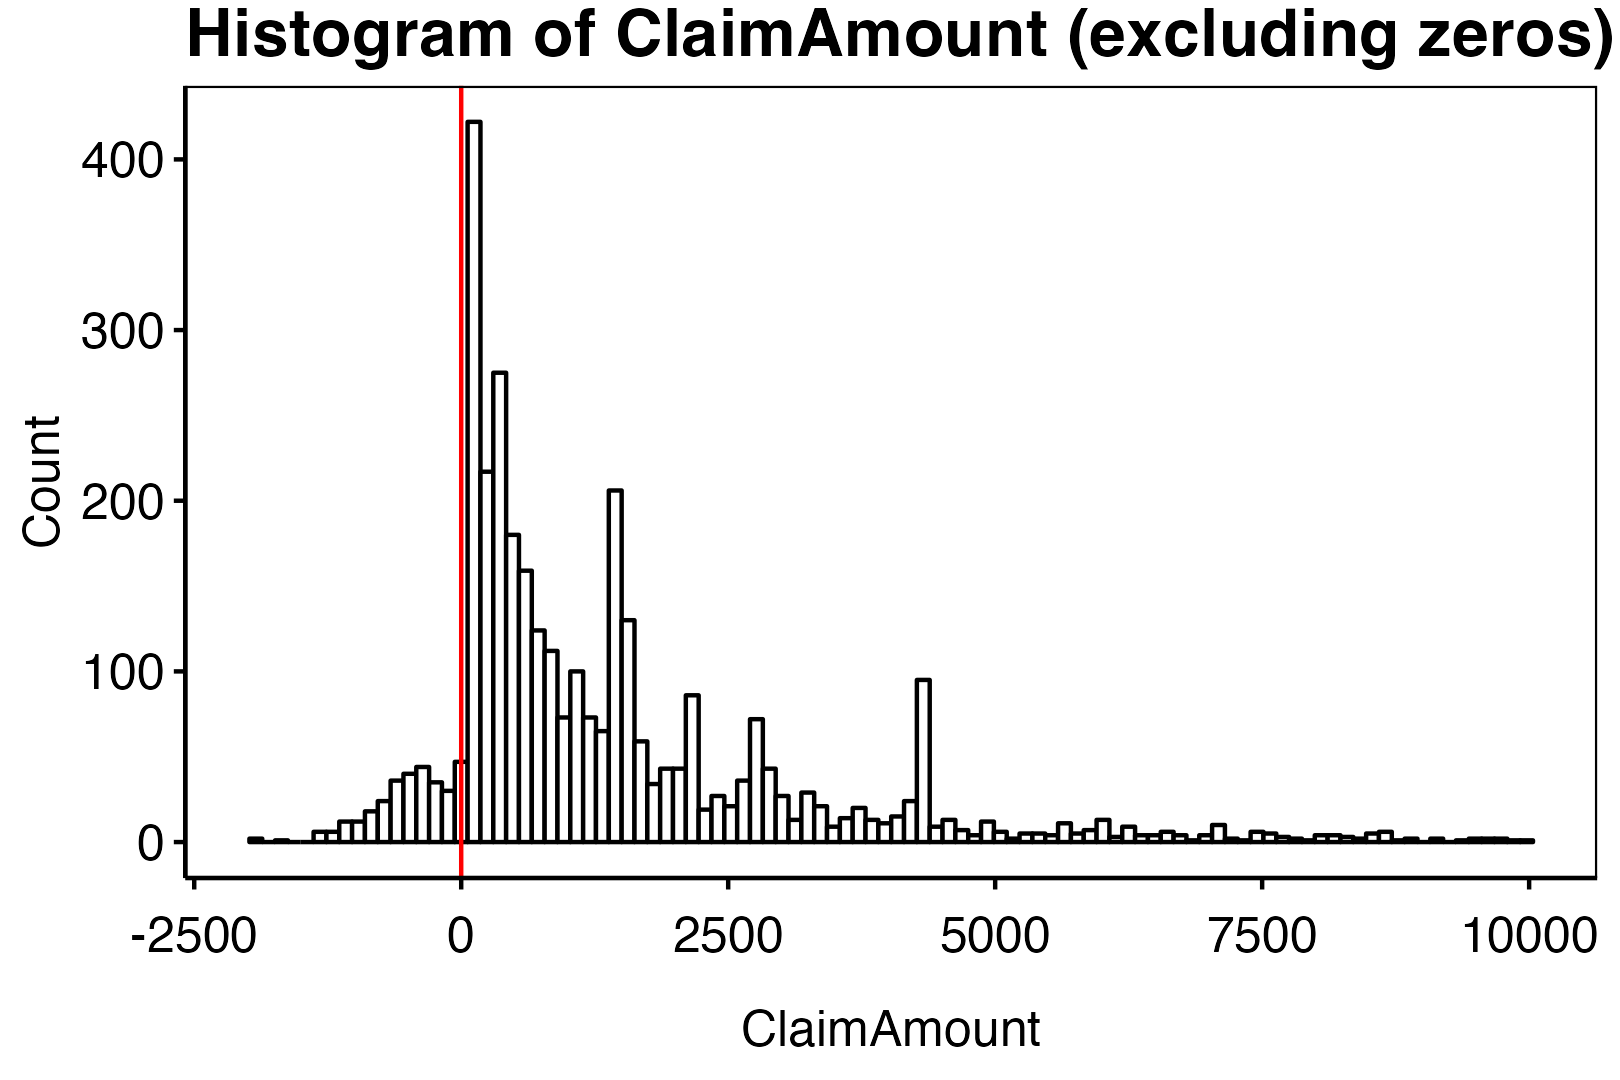
\includegraphics[width=0.48\textwidth]{figures/plot1.png}
  \end{center}
  \caption{Histogram of the variable `ClaimAmount`.}
\end{wrapfigure}

\textbf{Missing values.} As with any statistical modelling we start by
doing some exploratory analysis of the data \texttt{freMPL1}. As it was
seen in the previous section, the number of variables (columns) missing
datapoints were only one. The one in question is \texttt{RecordEnd}
which has 14143 out of 30595 missing values. This does not bather us
since we have the variable \texttt{Exposure} giving the time difference
between \texttt{RecordBeg} and \texttt{RecordEnd} in calendar years.
Furthermore we have that \texttt{RecordBeg} ranges from 2004-01-01 to
2004-12-31 and \texttt{RecordBeg\ +\ 365.25*Exposure} being at most
2004-12-31 meaning that all contracts span within the year 2004.
Assuming no seasonality trends this would incentivice us to remove the
two variables \texttt{RecordBeg} and \texttt{RecordEnd}.

\textbf{ClaimAmount and ClaimInd.} The variable of interest,
\texttt{ClaimAmount}, excibits a strange behaviour as it contains 285
strictly negative values. This is seen in figure 1. As this does not
intuitively makes sense we will set these values as zero and ensure that
the \texttt{ClaimInd} reflects this change.

\textbf{VehEngine and VehEnergy.} \emph{(Vehicle specific, 1)} Regarding
the categorical variables we notice that some levels is has sparse data.
The variables \texttt{VehEngine} and \texttt{VehEnergy} has both the
levels \texttt{GPL} and \texttt{electric}. We do however not have any
substantial datapoints as in total these levels contain 8 observations.
As the total dataset has 30595 observations in total we choose to remove
these observations.

\begin{figure}[h]
    \centering
    \subfloat[\centering]{{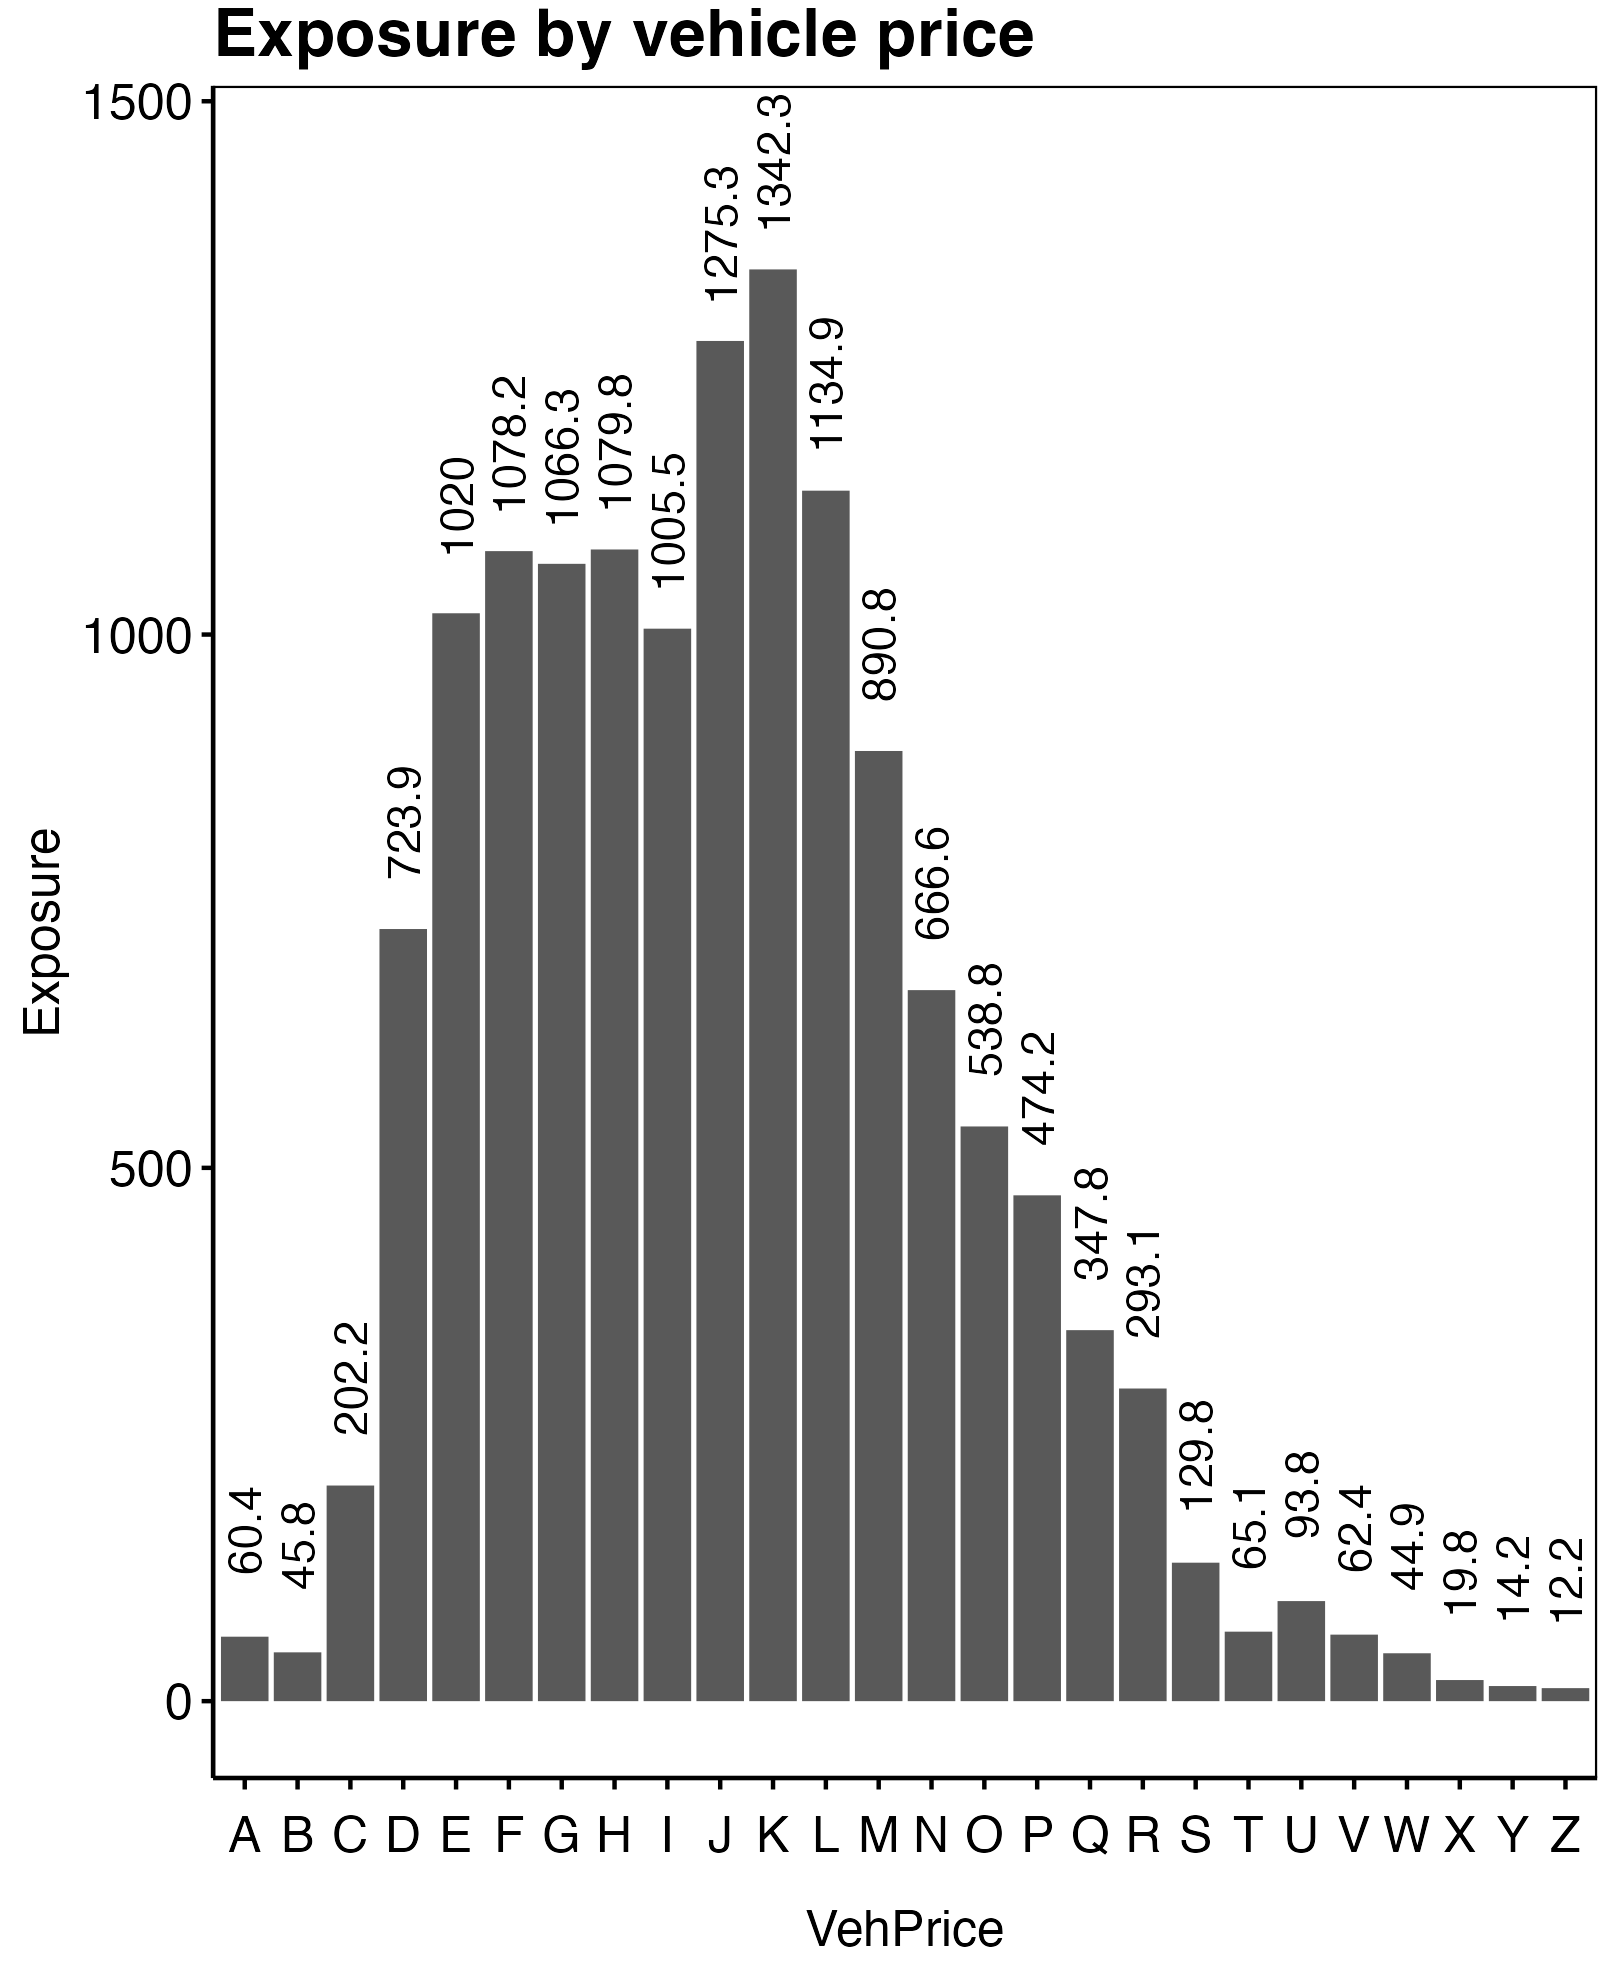
\includegraphics[width=0.25\textwidth]{figures/plot5.png} }}
    \qquad
    \subfloat[\centering]{{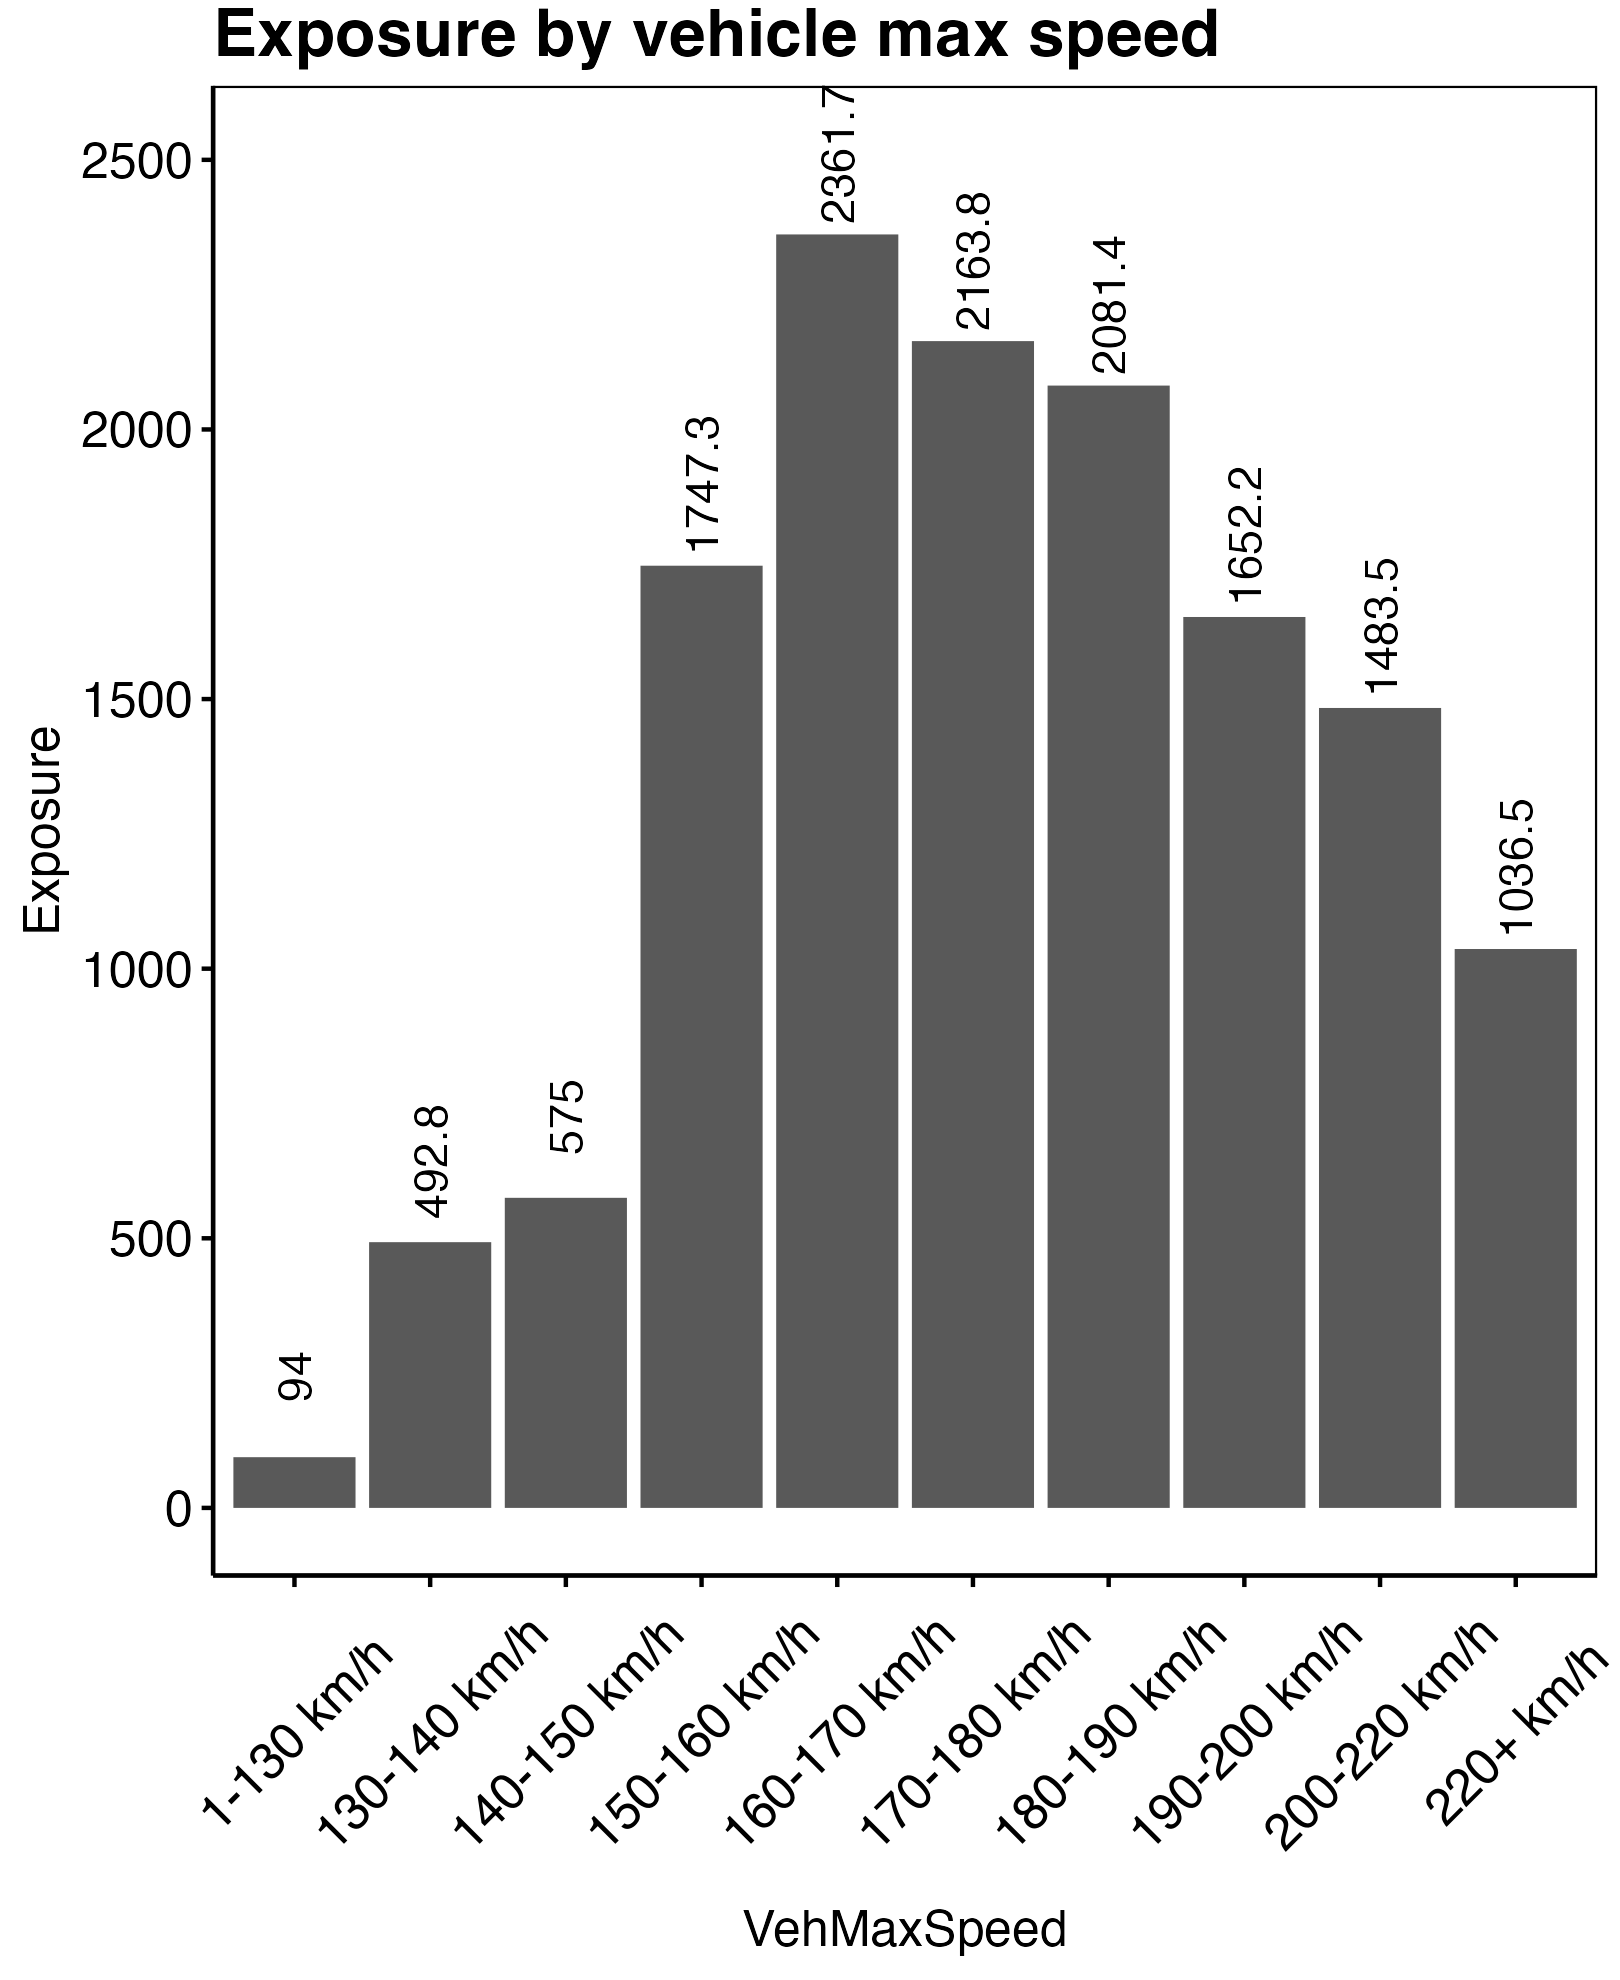
\includegraphics[width=0.25\textwidth]{figures/plot6.png} }}
    \qquad
    \subfloat[\centering]{{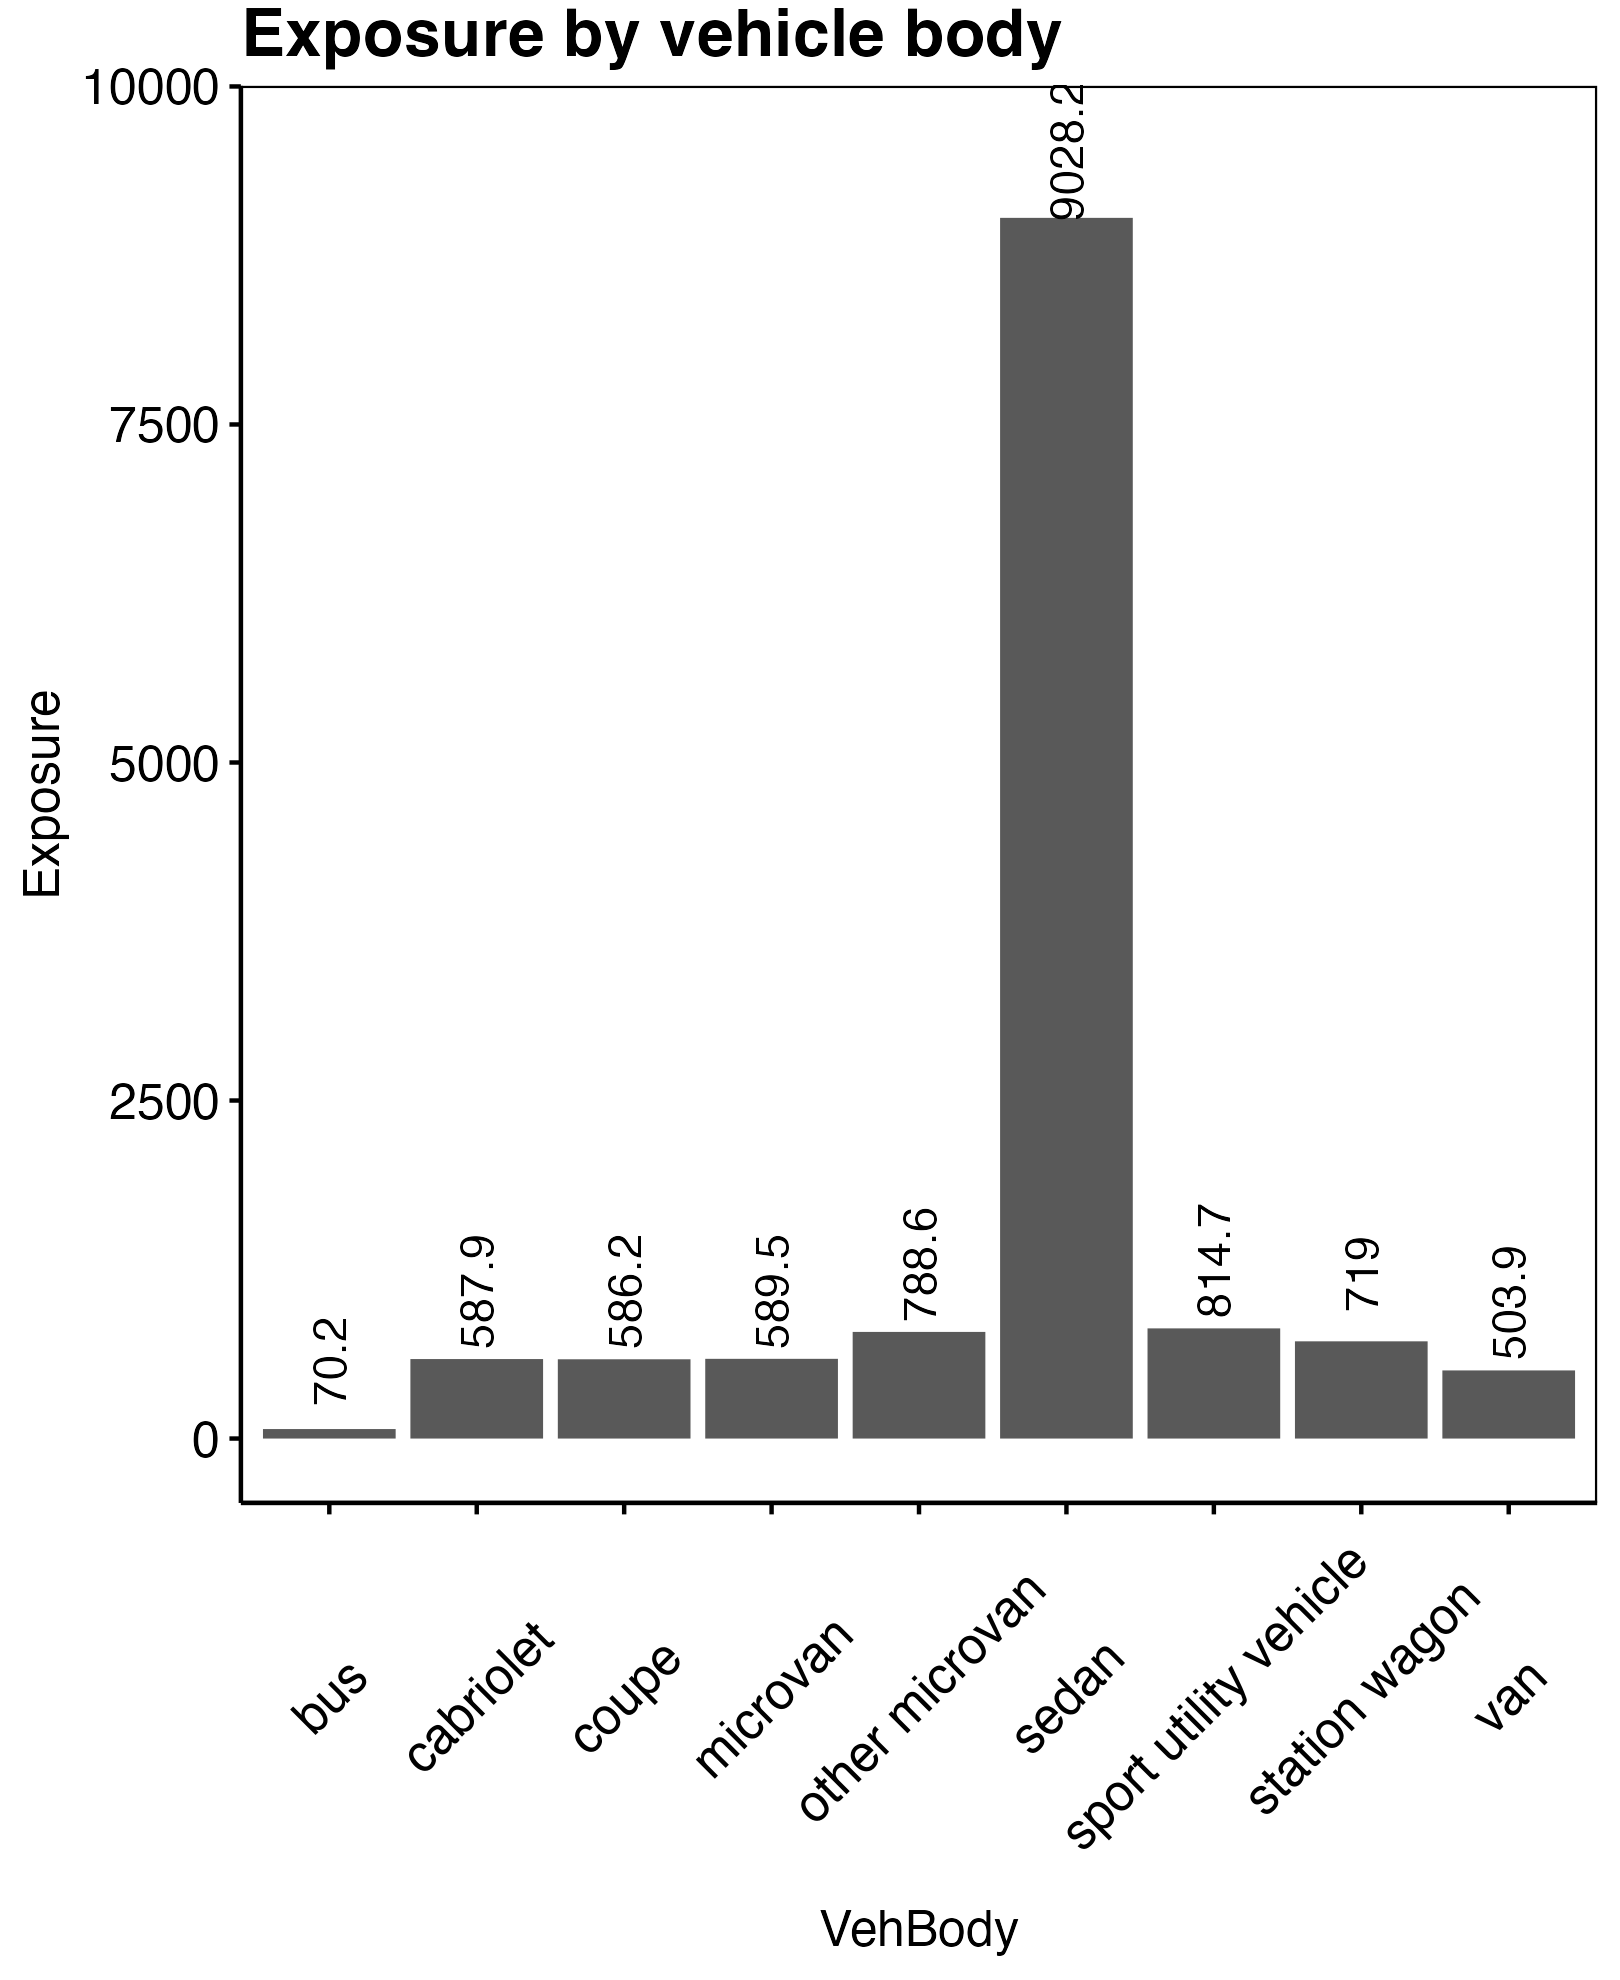
\includegraphics[width=0.25\textwidth]{figures/plot7.png} }}
    \caption{Exposure by respectively vehicle price (a), max speed (b) and body (c).}
\end{figure}

\textbf{VehPrice, VehMaxSpeed and VehBody.} \emph{(Vehicle specific, 2)}
In figure 2 we see that \texttt{VehPrice} is well represented in most
price categories. We do however har a shorter supply of data in the
tails. We will therefore combine the lowest three categories A through
C, the levels R through T and lastly U through Z. Regarding to the
vehicle max speed we see that a very few number of observations are in
the lowest category \texttt{1-130\ kmh}. We therefore combine the lowest
level with the level \texttt{130-140\ kmh}. The only vehicle body with
very few observations is \texttt{bus} with only 159 observations. We do
however see that \texttt{bus} act much like the category \texttt{sedan}
with respect to frequency and severity and so these are combined under
\texttt{sedan}.

\textbf{VehAge, VehUsage and VehClass.} \emph{(Vehicle specific, 3)} The
remaining three vehicle specific variable is well represented throughout
all levels. The only scarce observation is \texttt{VehUsage} being
\texttt{Professional\ run}. We therefore combine \texttt{Proffesional}
and \texttt{Professional\ run} under \texttt{Professional}. We leave the
remaining levels as is.

\begin{wrapfigure}{r}{0.40\textwidth}
  \begin{center}
    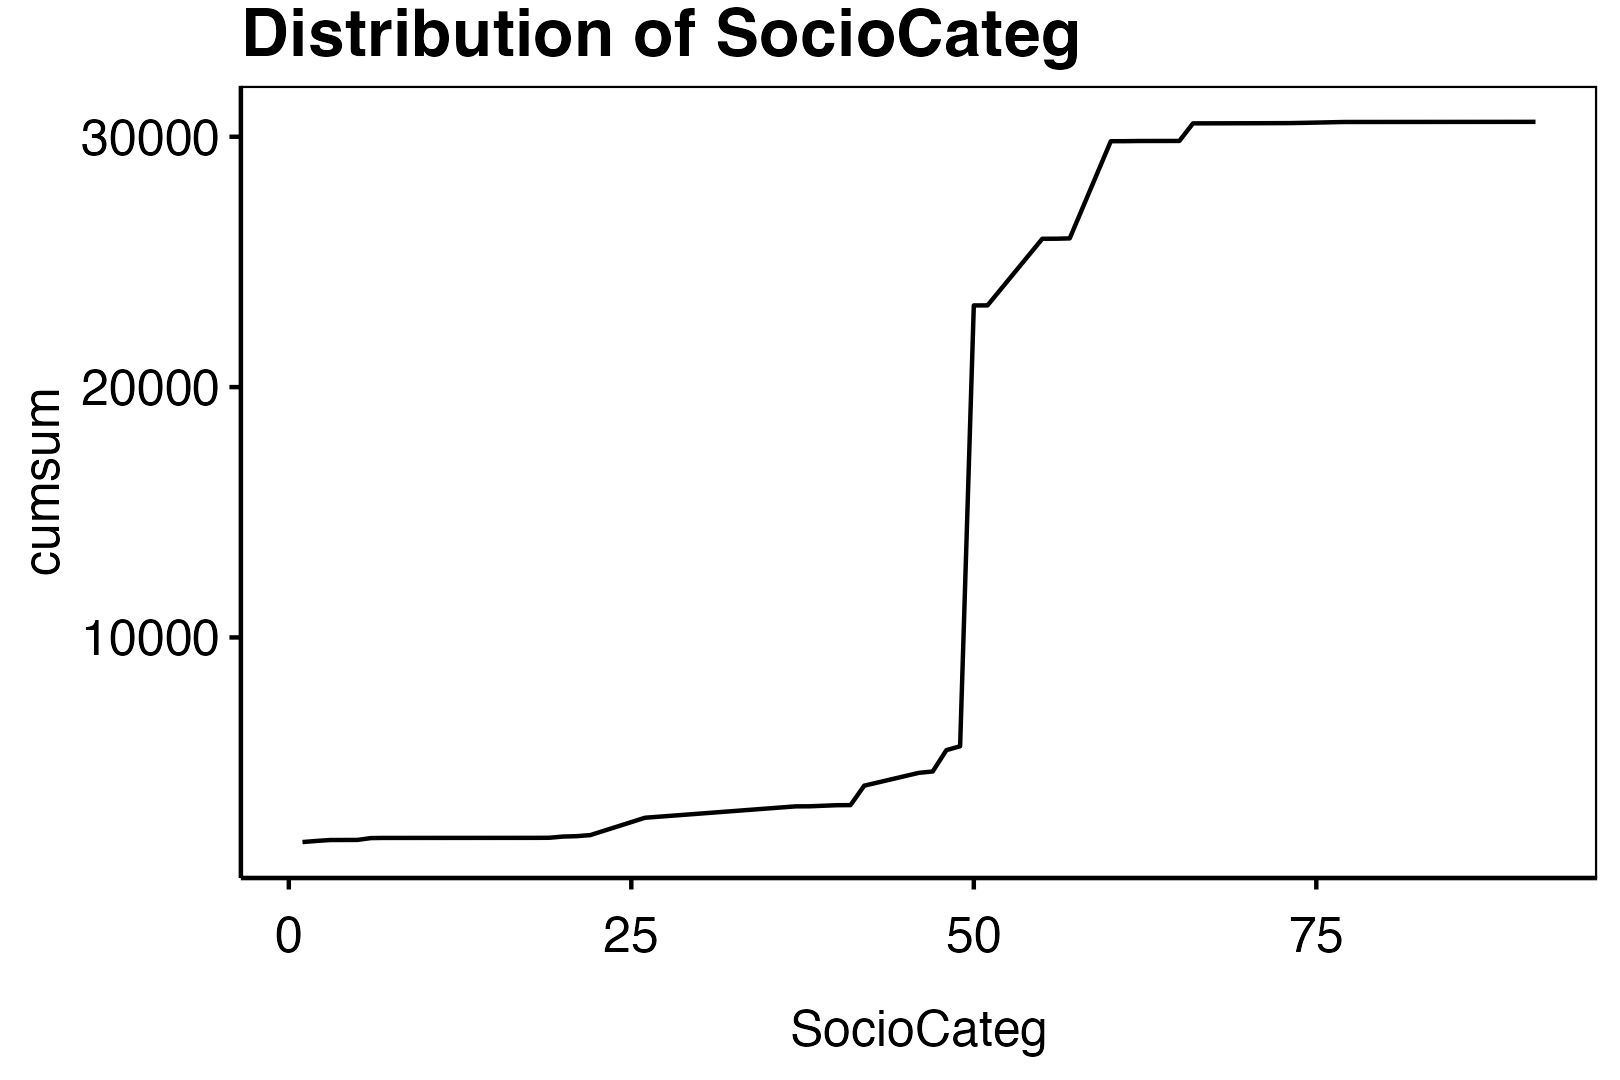
\includegraphics[width=0.38\textwidth]{figures/plot4.png}
  \end{center}
  \caption{Cummulative distribution of the variable `SocioCateg`.}
\end{wrapfigure}

\textbf{SocioCateg and Gender.} \emph{(Socails)} When constructing a
statistical model, one does not simply have to consider which variables
have the most explanatory value but one also have to take into
consideration the lawfullness of discriminating customors based on
covariates as gender, race and so forth. It is common knowledge that
insurance companies cannot discriminate based on gender and so we will
not use the variable \texttt{gender} as explanatory variable even though
it might improve the model predictions. The variable \texttt{SocioCateg}
representing the socioeconomic status of the insured ranges between
category 1 and 99. It is not at the moment clear whether this is a
covariate that may be used in pricing, so we will prefer not using it.
However, if it does indeed improve the fit without overfitting, we may
get some additional information from this variable. The data is indicate
that the custumors in general are in the category 50 with a few other
levels having significant more observations than others. For this reason
we combine the catagories from 1 to 49 into \texttt{A} and the
catagories 51 to 99 into \texttt{C} and keep the category \texttt{B} as
is.

\textbf{LicAge, DrivAge and MariStat.} \emph{(Customer specific)} In
general in France, one can acquire a drivers license at the age of 18
and so we have the obvious restriction
\texttt{LicAge\ \textless{}=\ DrivAge\ -\ 18} and we will in general
have that the license age will be approximately 18 years less than the
drivers license. It is therefore reasonable to discuss whether to
include both variables. We would however assume that for an older person
the license age would be more important than for youngsters.
Furthermore, we would assume that the \texttt{ClaimInd} and the
\texttt{LicAge} are negative correlated. We will therefore include both.
Both \texttt{Alone} and \texttt{Other} is well represented in
\texttt{MariStat}.

\textbf{HasKmLimit, RiskVar, Garage and BonusMalus} \emph{(Policy
related and others)} The variables remaining HasKmLimit, RiskVar, Garage
and BonusMalus are well represented throughout all levels and so no
action is taken here.

\begin{figure}[h]
  \begin{center}
    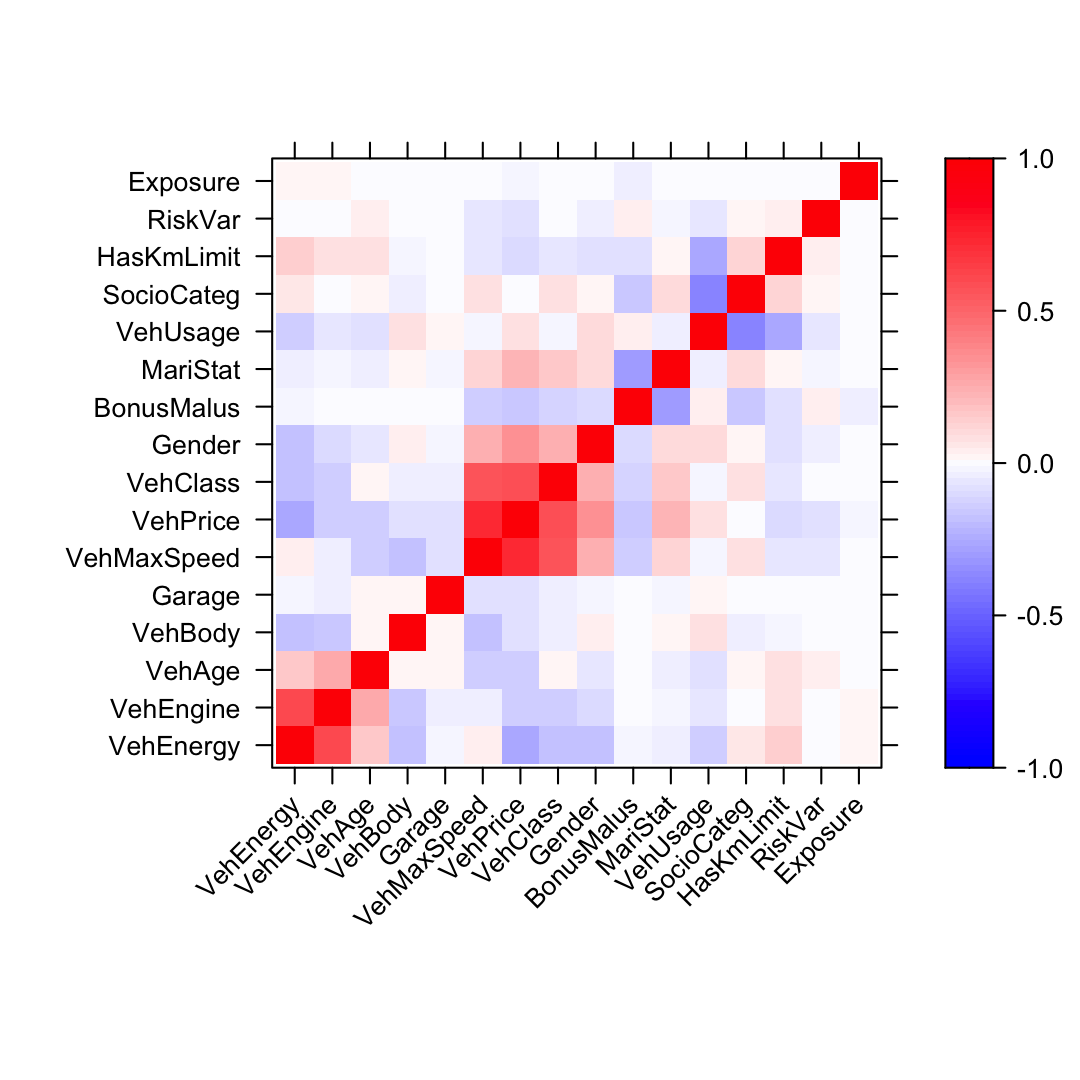
\includegraphics[width=0.48\textwidth]{figures/plot8.png}
  \end{center}
  \caption{Spearman correlation matrix.}
\end{figure}

\textbf{Correlations.} As discussed previously the age of the driver and
the license age i very correlated and so one may consider whether or not
both variables are needed. In practice we do however see that age and
experience are used when modelling the premium. Secondly, we see that
the covariates vehicle engine and energy are very correlated and also
the three variables vehicle max speed, price and class are well
correlated. Thirdly, we see that vehicle usage and socio category are
correlated. This is likely because wealthier people more often have a
car for professional use.

\newpage

\hypertarget{training-a-regression-model}{%
\section{Training a regression
model}\label{training-a-regression-model}}

The technical premium is based upon a frequency/severity model. We have
the base model assumptions as: Let \(Y:=Y_{t+\Delta t}\) be the claim
risen by a policy during the interval \([t,t+\Delta t)\) with
\(\Delta t\) representing the exposure. Notice that in princible
\(\Delta t\) is a stopping time defined as

\[
\Delta t := \min\big(1,\inf\{s\ge t : Y_s>0\}\big),
\] meaning the policy is terminated at the time \(t+\Delta t\) with
\(t+\Delta t=t+1\) if \(Y=0\). Notice that the exposure is censored if
\(\Delta t_i<1\) and \(Y_i=0\). We furthermore have the covariates
\(X\in \mathcal X\) with \(\mathcal X\) being a \(p\)-dimensional space.
We are interested in the object \(\mathbb E[Y\ \vert\ X]\) being the
expected claim risen given the covariates \(X\). Our main assumption is
that this expectation is decomposed into

\[
\mathbb E[Y\ \vert\ X]=\mathbb E[Y1_{Y>0}\ \vert\ X]=\mathbb E[Y\ \vert\ X,1_{Y>0}]\cdot \mathbb E[1_{Y>0}\ \vert\ X]=\mu_X\cdot p_X,
\]

where \(\mu_X\) is the expected claim in the event, that a claim arises
i.e.~the severity and \(p_X\) is the probability that a claim arises
i.e.~the frequency. However since the data is censored with exposure
\(\tilde{\Delta t}\le \Delta t\) we need to consider how we may
translate a predictive model into a price function for new policies. In
practice, we include exposure as a covariate.

We will search for the most efficient estimators for both the severity
and frequency. We will denote these estimators by \(m_\mu(X)\) and
\(m_p(X)\) where we will denote the model by a superscript \(m^{(*)}_j\)
with \(*\) denoting the model for \(j=\mu,p\).

\hypertarget{modelling-severity}{%
\subsection{Modelling severity}\label{modelling-severity}}

We model the severity by modelling
\texttt{ClaimAmount\ \textasciitilde{}\ X\_1\ +\ X\_2\ +\ ...} for
\texttt{X\_i} being either a numerical variable or a 0/1 variable. As
the response is numerical we choose the \(L^2\) loss given by the loss
function

\[
L(y_1,y_2)=(y_1-y_2)^2.
\]

We will by default not use any other feature selection as described in
the previous sections. We will start by testing which of the following
five models does best under the \(L^2\) loss

\begin{enumerate}
\def\labelenumi{\arabic{enumi}.}
\tightlist
\item
  The generalized additive model,
\item
  Elastic net linear model,
\item
  eXtreme Gradient Boosting or short XGBoost,
\item
  Bayesian Additive Regression Tree or shot BART,
\item
  Random forests implemented through \texttt{ranger}.
\end{enumerate}

\hypertarget{generalized-additive-model}{%
\subsubsection{Generalized Additive
Model}\label{generalized-additive-model}}

The generalized additive model we do not necessary assume that
\(Y\ \vert\ X\) is normal distributed and may be modeled as a linear
combination of features. Instead we assume that the conditional mean
satisfies the following

\[
g\left(\mathbb E[Y\ \vert\ X]\right)=\beta_0 + \sum_{i=1}^pf_i(X_i):=\eta \tag{1}
\]

where \(g\) is the link function relating the parameter \(\eta\) with
the mean. The functions \(f_i\) for \(i=1,...,p\) are smoothing
functions. Furthermore we in general assume that
\(Y\ \vert\ X\sim \mathcal E\) for some exponential distribution.
However in this case we choose the link function \(g(x)=x\) (identity)
and the response distribution as gaussian, that is we assume the model

\[
Y\ \vert\ X=\beta_0 + \sum_{i=1}^pf_i(X_i)+\varepsilon,
\]

with \(\varepsilon\sim\mathcal N(0,\sigma^2)\). For the smoothing
functions we choose splines and apply them to the continuous variables
\texttt{LicAge}, \texttt{BonusMalus} and \texttt{DrivAge}. The rest of
the variables are indicators and so no smoother is applied. Fitting this
model to the training data and predicting onto the test data yields the
below pairs \texttt{(truth,response)}.

\begin{figure}[h]
    \centering
    \subfloat[\centering]{{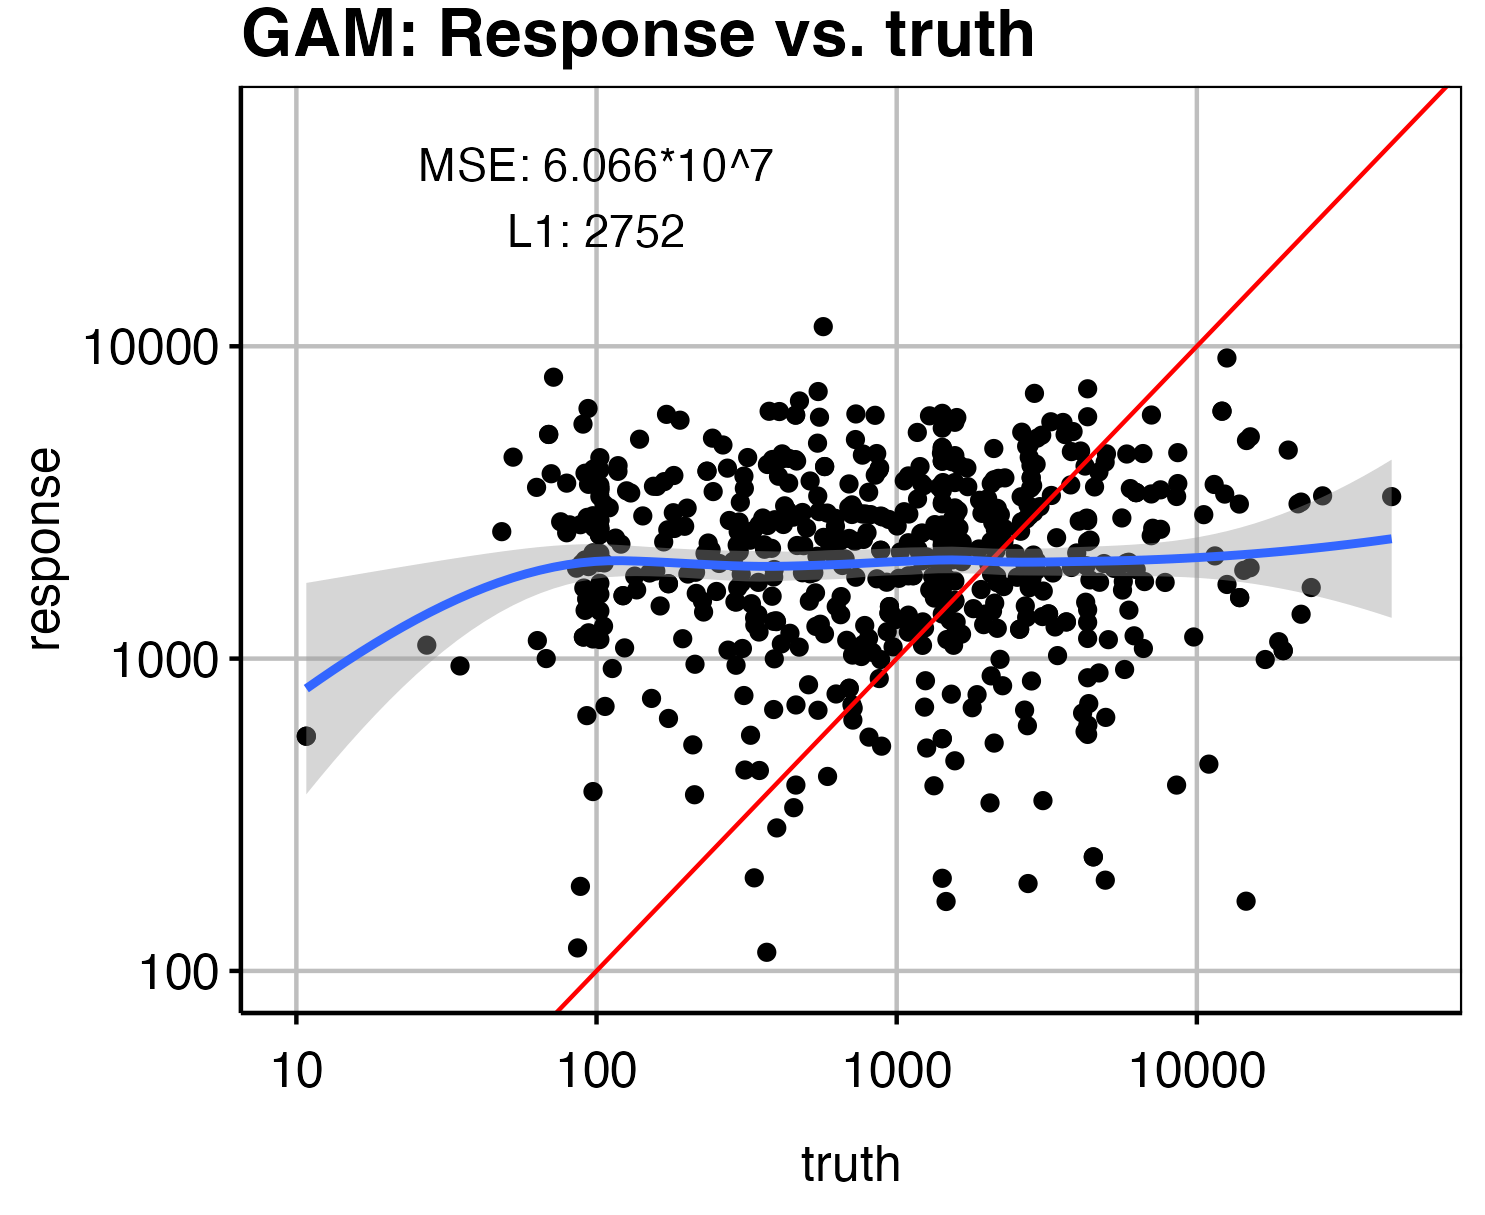
\includegraphics[width=0.34\textwidth]{figures/sev_p_gam_wide.png} }}
    \qquad
    \subfloat[\centering]{{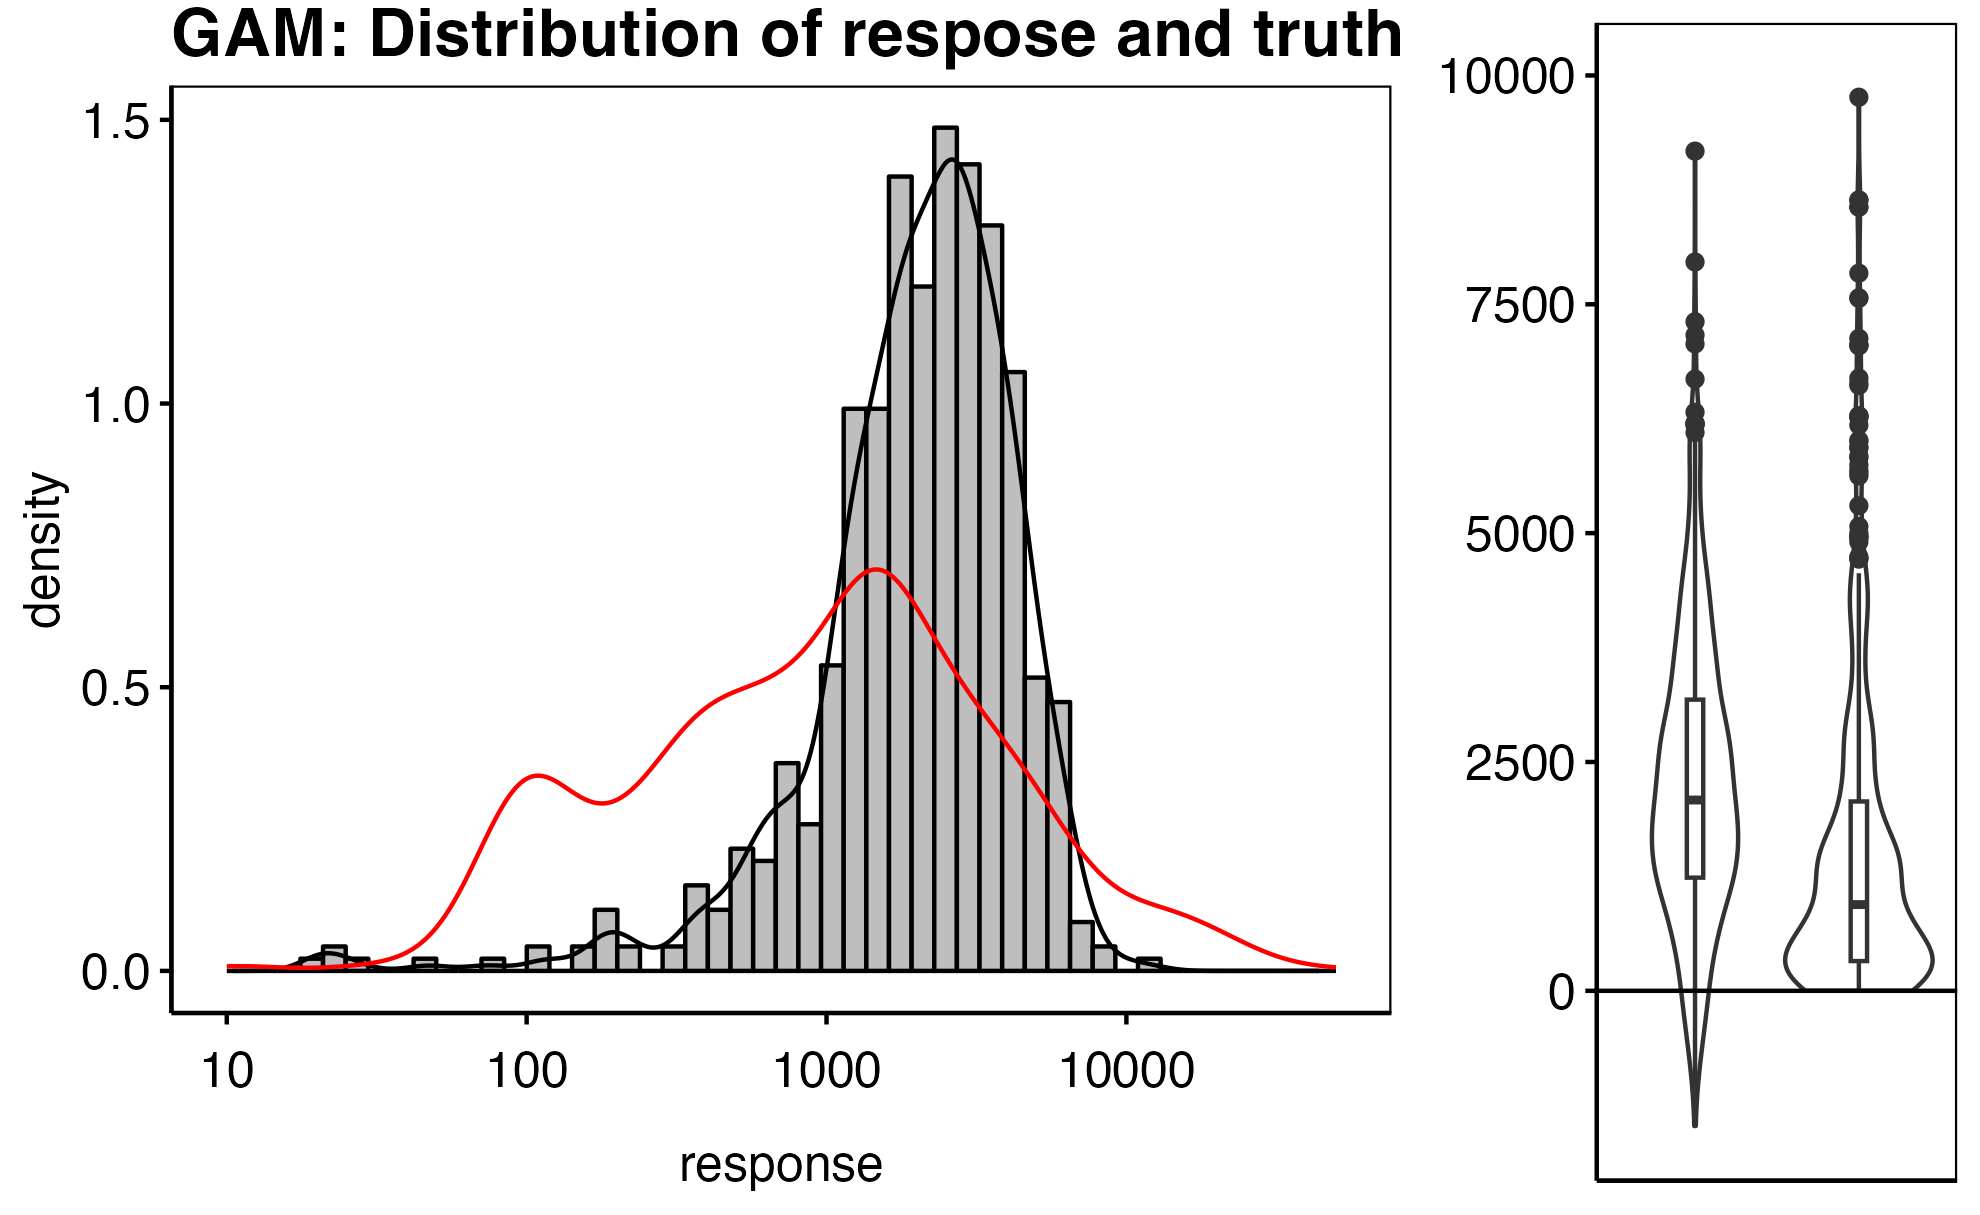
\includegraphics[width=0.46\textwidth]{figures/sev_p_gam3.png} }}
    \caption{(a): Predictions for the GAM with x being the actual value and y being the estimate. The red line represent the mapping $y=x$. (b, left): Distribution of the response and actual values. The red density function represents the empirical density of the test data set. (b, right): A combined boxplot and violin plot of the distribution of the response (left) and the actual value (right).}
\end{figure}

One sees that the model predicts negative claims. This is obviously
problematic since this would imply that the technical premium would be
negative as well. Other than this, the model does a poor job in
capturing the heavy tail of the true distribution. This is not a problem
with the model but rather a lack of extreme value considerations.

We can check the model predictions on a couple of specific policies,
namely the row numbers 6257, 25018, 30503 and 30563. Let us briefly take
a look at the four policies.

\begin{table}[!h]

\caption{\label{tab:unnamed-chunk-13}Policy covariates for policies of interest (6257, 24131, 25018, 25196, 30503 and 30563).}
\centering
\resizebox{\linewidth}{!}{
\begin{tabular}[t]{lrrllllrrrllllllrrlrr}
\toprule
  & Exposure & LicAge & VehAge & MariStat & SocioCateg & VehUsage & DrivAge & HasKmLimit & BonusMalus & VehBody & VehPrice & VehEngine & VehEnergy & VehMaxSpeed & VehClass & ClaimAmount & RiskVar & Garage & ClaimInd & id\\
\midrule
6254 & 0.083 & 274 & 3 & Alone & B & Private+trip to office & 42 & 0 & 50 & sedan & F & injection & regular & 160-170 km/h & B & 0.000 & 17 & None & 0 & 6257\\
24123 & 0.200 & 0 & 3 & Alone & A & Private+trip to office & 18 & 0 & 100 & coupe & F & injection overpowered & regular & 1-140 kmh & A & 3067.356 & 16 & None & 1 & 24131\\
25010 & 0.103 & 1 & 3 & Alone & A & Private+trip to office & 18 & 0 & 100 & sedan & G & direct injection overpowered & diesel & 160-170 km/h & B & 0.000 & 8 & None & 0 & 25018\\
25188 & 0.083 & 276 & 1 & Alone & B & Private+trip to office & 42 & 0 & 50 & sedan & H & direct injection overpowered & diesel & 160-170 km/h & B & 0.000 & 3 & None & 0 & 25196\\
30495 & 0.052 & 703 & 8-9 & Other & C & Private & 89 & 0 & 50 & cabriolet & M & injection & regular & 180-190 km/h & M1 & 0.000 & 1 & Collective garage & 0 & 30503\\
\addlinespace
30555 & 0.408 & 855 & 10+ & Other & C & Private & 89 & 0 & 50 & sedan & G & injection & regular & 160-170 km/h & B & 0.000 & 12 & None & 0 & 30563\\
\bottomrule
\end{tabular}}
\end{table}

Then applying the estimator we obtain the estimates.

\begin{longtable}[]{@{}
  >{\centering\arraybackslash}p{(\columnwidth - 16\tabcolsep) * \real{0.1111}}
  >{\centering\arraybackslash}p{(\columnwidth - 16\tabcolsep) * \real{0.1111}}
  >{\centering\arraybackslash}p{(\columnwidth - 16\tabcolsep) * \real{0.1111}}
  >{\centering\arraybackslash}p{(\columnwidth - 16\tabcolsep) * \real{0.1111}}
  >{\centering\arraybackslash}p{(\columnwidth - 16\tabcolsep) * \real{0.1111}}
  >{\centering\arraybackslash}p{(\columnwidth - 16\tabcolsep) * \real{0.1111}}
  >{\centering\arraybackslash}p{(\columnwidth - 16\tabcolsep) * \real{0.1111}}
  >{\centering\arraybackslash}p{(\columnwidth - 16\tabcolsep) * \real{0.1111}}
  >{\centering\arraybackslash}p{(\columnwidth - 16\tabcolsep) * \real{0.1111}}@{}}
\toprule()
\begin{minipage}[b]{\linewidth}\centering
Estimator
\end{minipage} & \begin{minipage}[b]{\linewidth}\centering
\(\hat R_{L^2}\)
\end{minipage} & \begin{minipage}[b]{\linewidth}\centering
\(\hat R_{L^1}\)
\end{minipage} & \begin{minipage}[b]{\linewidth}\centering
6257
\end{minipage} & \begin{minipage}[b]{\linewidth}\centering
24131
\end{minipage} & \begin{minipage}[b]{\linewidth}\centering
25018
\end{minipage} & \begin{minipage}[b]{\linewidth}\centering
25196
\end{minipage} & \begin{minipage}[b]{\linewidth}\centering
30503
\end{minipage} & \begin{minipage}[b]{\linewidth}\centering
30563
\end{minipage} \\
\midrule()
\endhead
\(m^{(GAM)}_\mu\) & \(6.066\cdot 10^7\) & 2752.16 & 2463.49 & 4684.1 &
6047.67 & 2263.16 & 2009.47 & 1694.34 \\
\bottomrule()
\end{longtable}

\hypertarget{elastic-net-linear-model}{%
\subsubsection{Elastic net linear
model}\label{elastic-net-linear-model}}

\begin{figure}[h]
    \centering
    \subfloat[\centering]{{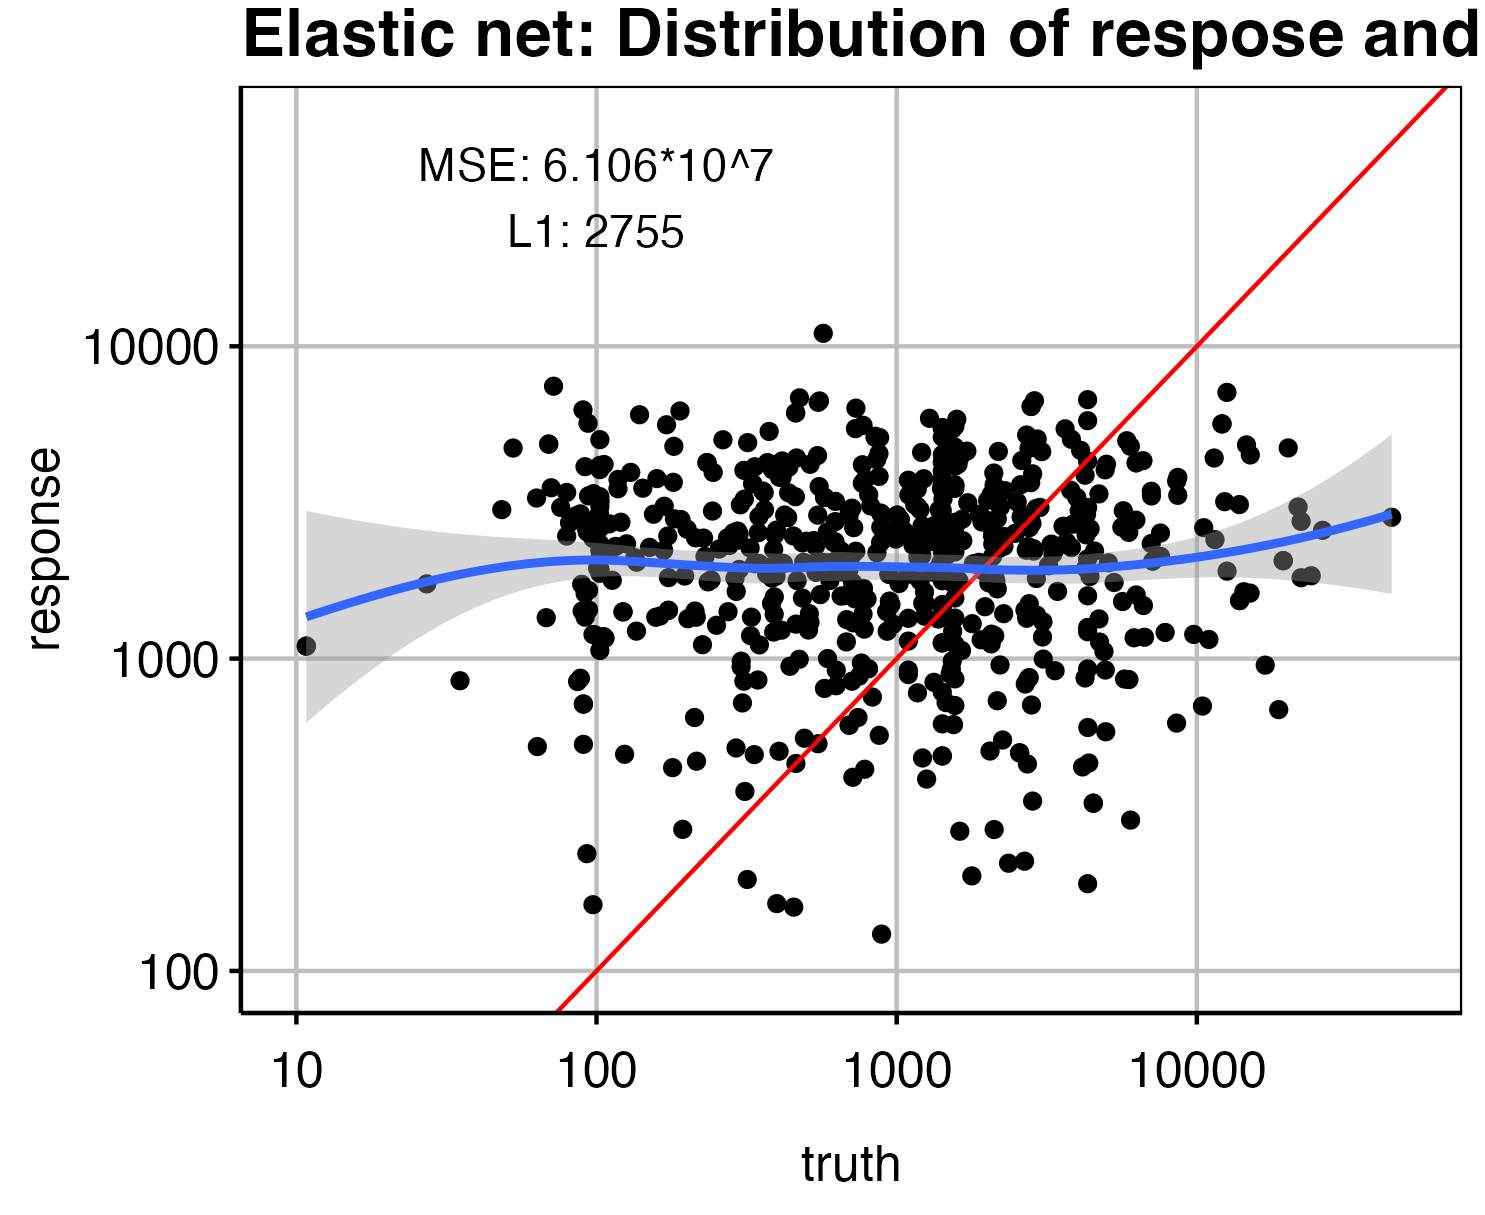
\includegraphics[width=0.34\textwidth]{figures/sev_p_glmnet_wide.png} }}
    \qquad
    \subfloat[\centering]{{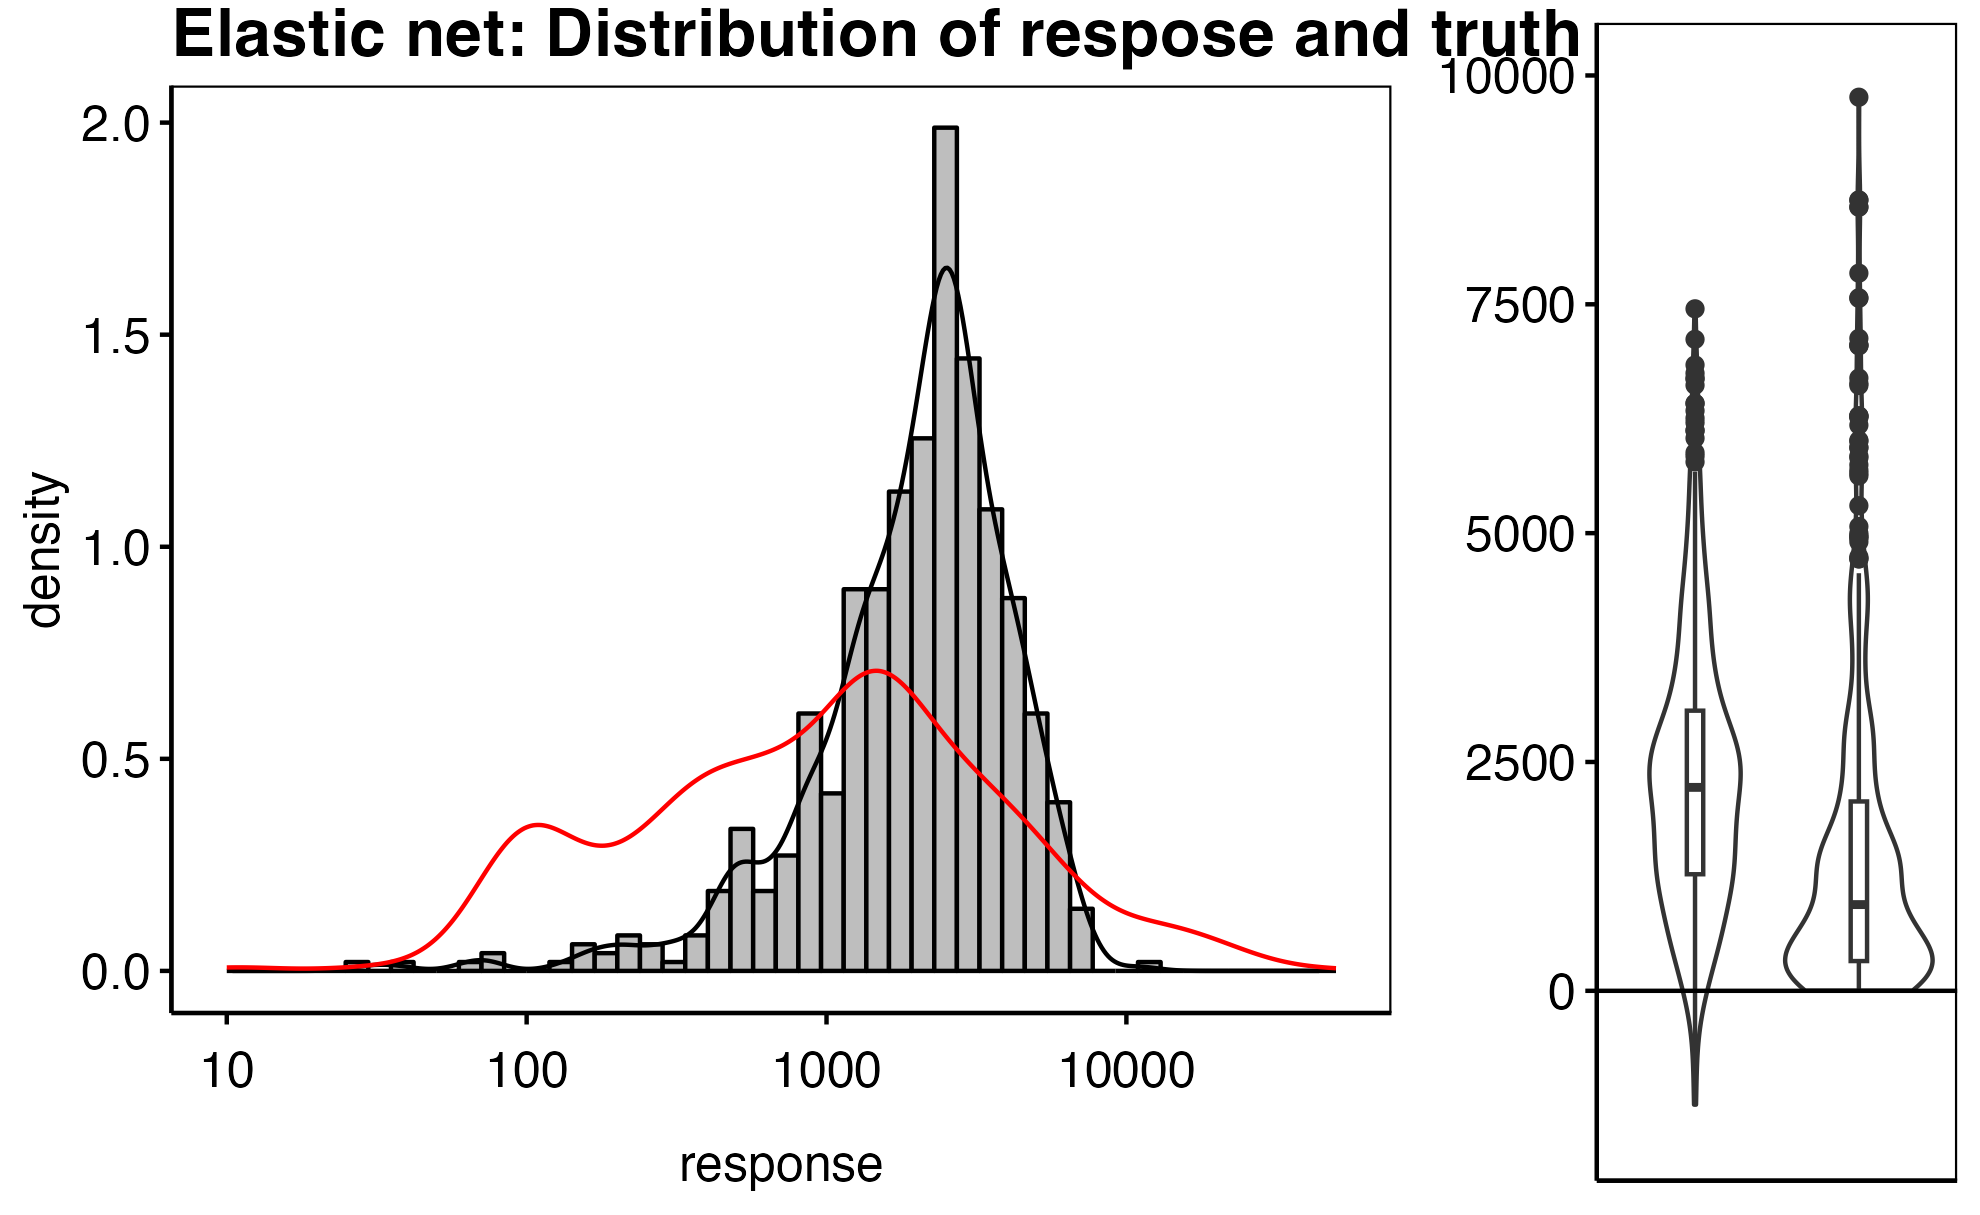
\includegraphics[width=0.46\textwidth]{figures/sev_p_glmnet3.png} }}
    \caption{(a): Predictions for the elastic net regression model with x being the actual value and y being the estimate. The red line represent the mapping $y=x$. (b, left): Distribution of the response and actual values. The red density function represents the empirical density of the test data set. (b, right): A combined boxplot and violin plot of the distribution of the response (left) and the actual value (right).}
\end{figure}

The elastic net is a penalized linear model where the estimate is based
on the algorithm

\[
m^{(EN)}_\mu(X)=\left(\beta_\lambda^{EN }\right)^\top X
\]

where \(\beta\)-parameter is determined through the minimization problem

\[
\hat{\beta}_\lambda^{\text {glmnet }} =\underset{\beta \in \mathbb{R}^p}{\arg \min }\left\{\hat{R}_n(\beta)+J_\lambda(\beta)\right\},\hspace{15pt}J_\lambda(\beta)=\lambda \left[\alpha\sum_{j=1}^p\left|\beta_j\right|+\frac{1-\alpha}{2}\sum_{j=1}^p\beta_j^2\right].
\]

Through 5-fold cross validation we choose the parameters
\(\lambda = 0.205564\) and \(\alpha = 0.000963\). We may consider the
estimate for the policies from above.

\begin{longtable}[]{@{}
  >{\centering\arraybackslash}p{(\columnwidth - 16\tabcolsep) * \real{0.1111}}
  >{\centering\arraybackslash}p{(\columnwidth - 16\tabcolsep) * \real{0.1111}}
  >{\centering\arraybackslash}p{(\columnwidth - 16\tabcolsep) * \real{0.1111}}
  >{\centering\arraybackslash}p{(\columnwidth - 16\tabcolsep) * \real{0.1111}}
  >{\centering\arraybackslash}p{(\columnwidth - 16\tabcolsep) * \real{0.1111}}
  >{\centering\arraybackslash}p{(\columnwidth - 16\tabcolsep) * \real{0.1111}}
  >{\centering\arraybackslash}p{(\columnwidth - 16\tabcolsep) * \real{0.1111}}
  >{\centering\arraybackslash}p{(\columnwidth - 16\tabcolsep) * \real{0.1111}}
  >{\centering\arraybackslash}p{(\columnwidth - 16\tabcolsep) * \real{0.1111}}@{}}
\toprule()
\begin{minipage}[b]{\linewidth}\centering
Estimator
\end{minipage} & \begin{minipage}[b]{\linewidth}\centering
\(\hat R_{L^2}\)
\end{minipage} & \begin{minipage}[b]{\linewidth}\centering
\(\hat R_{L^1}\)
\end{minipage} & \begin{minipage}[b]{\linewidth}\centering
6257
\end{minipage} & \begin{minipage}[b]{\linewidth}\centering
24131
\end{minipage} & \begin{minipage}[b]{\linewidth}\centering
25018
\end{minipage} & \begin{minipage}[b]{\linewidth}\centering
25196
\end{minipage} & \begin{minipage}[b]{\linewidth}\centering
30503
\end{minipage} & \begin{minipage}[b]{\linewidth}\centering
30563
\end{minipage} \\
\midrule()
\endhead
\(m^{(EN)}_\mu\) & \(6.106\cdot 10^7\) & 2754.79 & 2338.48 & 1843.77 &
3206.72 & 2142.26 & 1143.72 & 1322.23 \\
\bottomrule()
\end{longtable}

\hypertarget{xgboost}{%
\subsubsection{XGBoost}\label{xgboost}}

\begin{figure}[h]
    \centering
    \subfloat[\centering]{{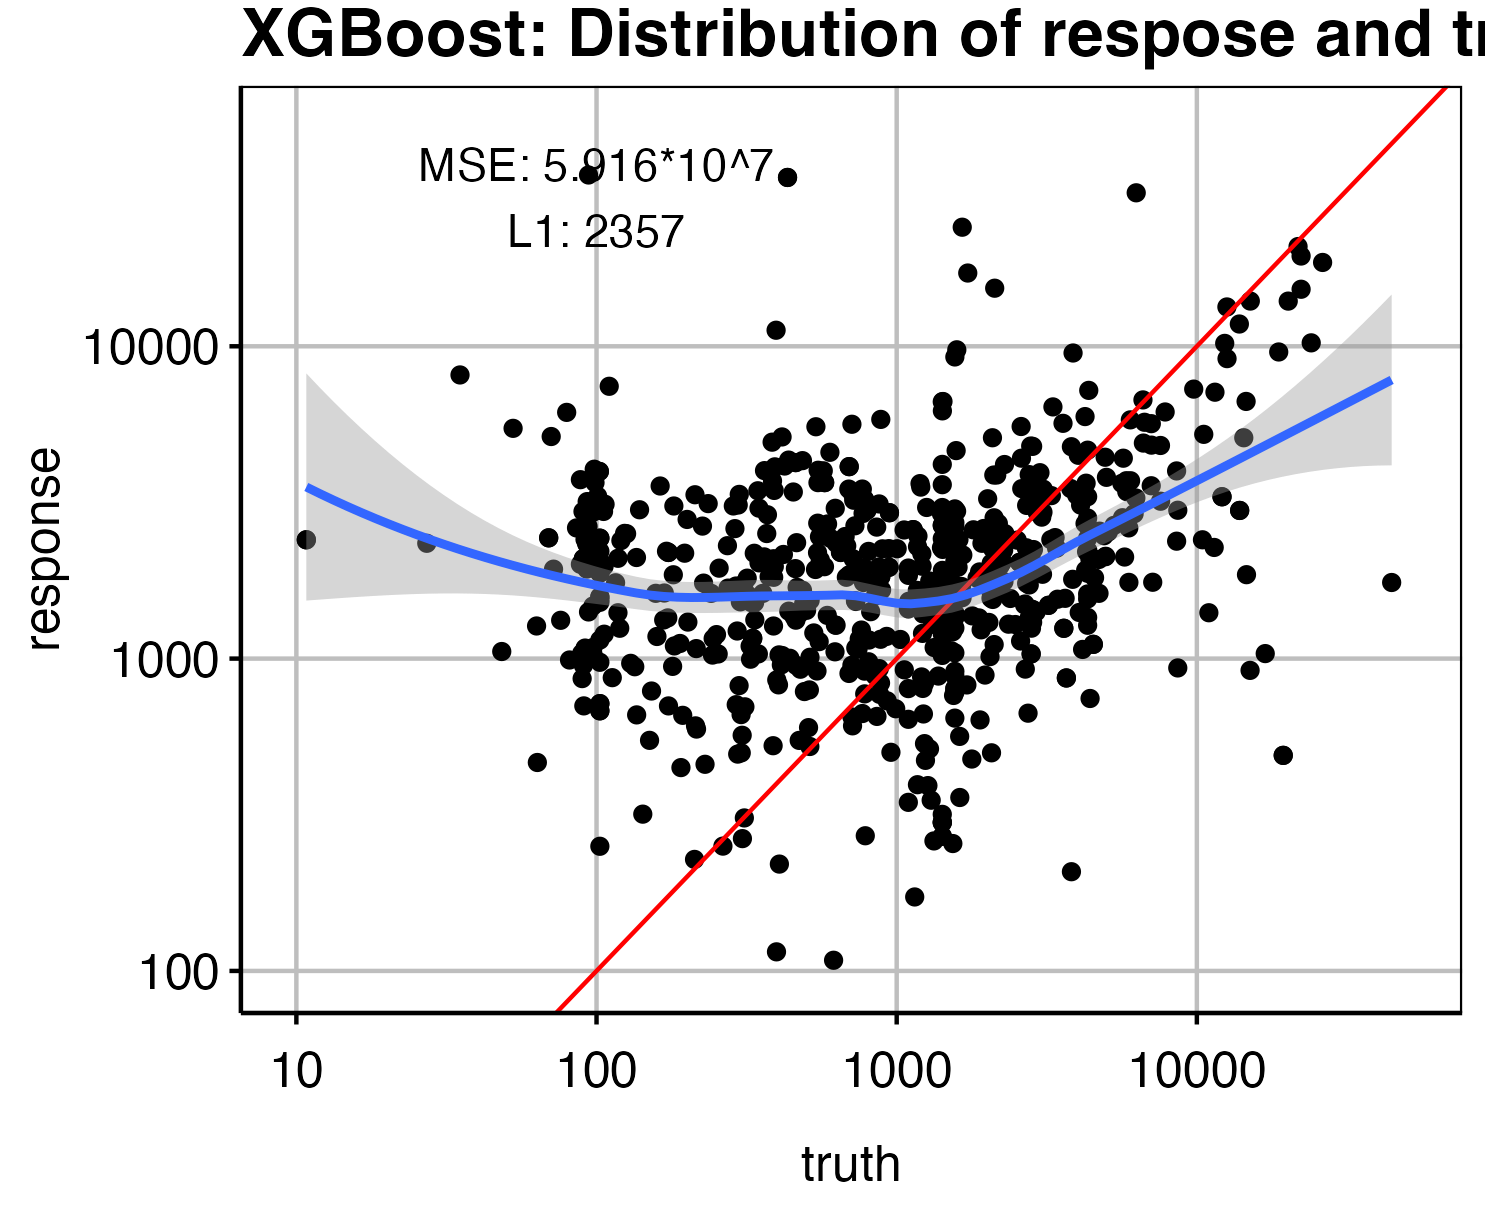
\includegraphics[width=0.34\textwidth]{figures/sev_p_xgboost_wide.png} }}
    \qquad
    \subfloat[\centering]{{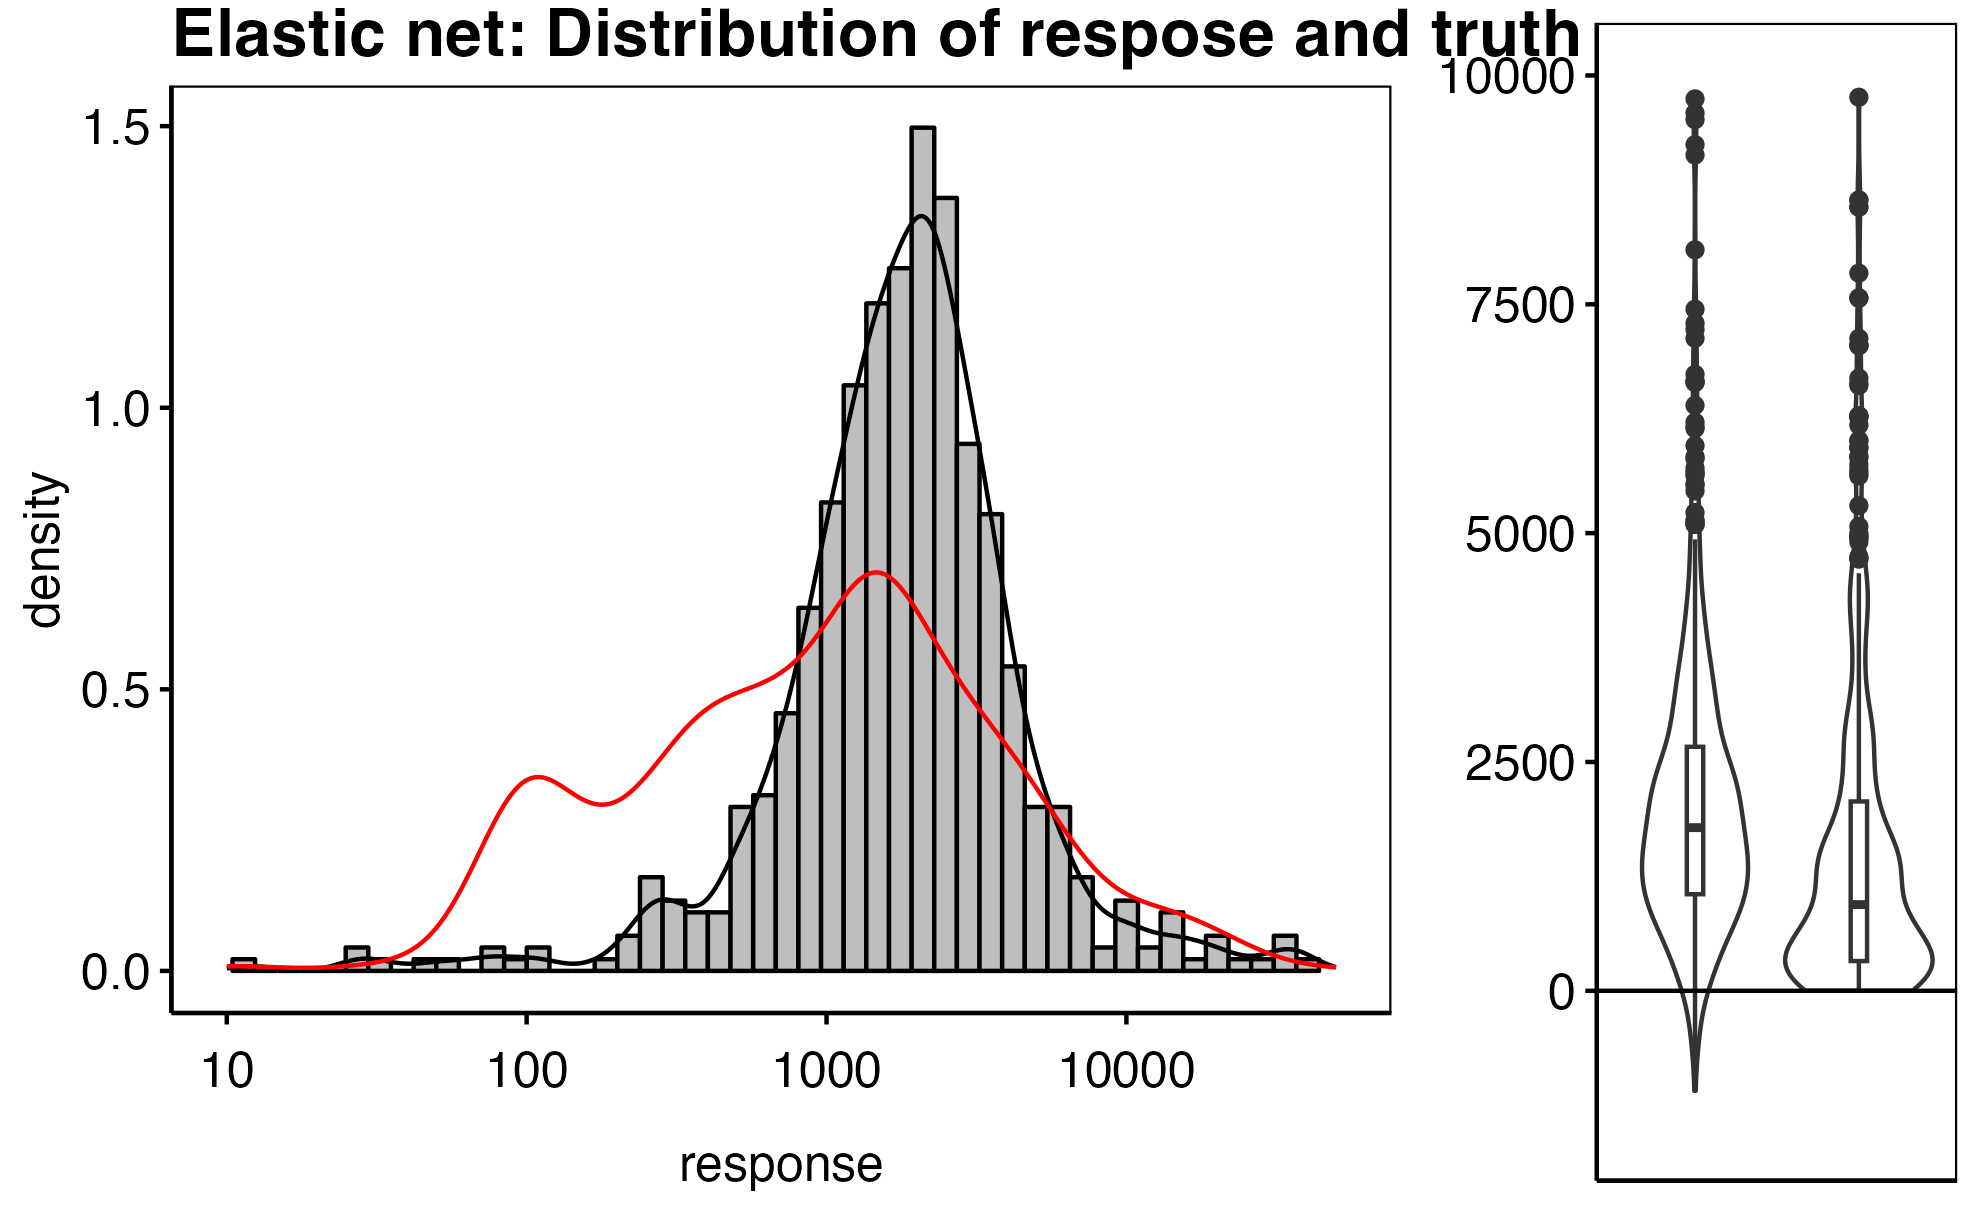
\includegraphics[width=0.46\textwidth]{figures/sev_p_xgboost3.png} }}
    \caption{(a): Predictions for the XGBoost regression model with x being the actual value and y being the estimate. The red line represent the mapping $y=x$. (b, left): Distribution of the response and actual values. The red density function represents the empirical density of the test data set. (b, right): A combined boxplot and violin plot of the distribution of the response (left) and the actual value (right).}
\end{figure}

\begin{longtable}[]{@{}
  >{\centering\arraybackslash}p{(\columnwidth - 16\tabcolsep) * \real{0.1111}}
  >{\centering\arraybackslash}p{(\columnwidth - 16\tabcolsep) * \real{0.1111}}
  >{\centering\arraybackslash}p{(\columnwidth - 16\tabcolsep) * \real{0.1111}}
  >{\centering\arraybackslash}p{(\columnwidth - 16\tabcolsep) * \real{0.1111}}
  >{\centering\arraybackslash}p{(\columnwidth - 16\tabcolsep) * \real{0.1111}}
  >{\centering\arraybackslash}p{(\columnwidth - 16\tabcolsep) * \real{0.1111}}
  >{\centering\arraybackslash}p{(\columnwidth - 16\tabcolsep) * \real{0.1111}}
  >{\centering\arraybackslash}p{(\columnwidth - 16\tabcolsep) * \real{0.1111}}
  >{\centering\arraybackslash}p{(\columnwidth - 16\tabcolsep) * \real{0.1111}}@{}}
\toprule()
\begin{minipage}[b]{\linewidth}\centering
Estimator
\end{minipage} & \begin{minipage}[b]{\linewidth}\centering
\(\hat R_{L^2}\)
\end{minipage} & \begin{minipage}[b]{\linewidth}\centering
\(\hat R_{L^1}\)
\end{minipage} & \begin{minipage}[b]{\linewidth}\centering
6257
\end{minipage} & \begin{minipage}[b]{\linewidth}\centering
24131
\end{minipage} & \begin{minipage}[b]{\linewidth}\centering
25018
\end{minipage} & \begin{minipage}[b]{\linewidth}\centering
25196
\end{minipage} & \begin{minipage}[b]{\linewidth}\centering
30503
\end{minipage} & \begin{minipage}[b]{\linewidth}\centering
30563
\end{minipage} \\
\midrule()
\endhead
\(m^{(XGB)}_\mu\) & \(5.916\cdot 10^7\) & 2357.03 & 4416.08 & 3226.21 &
6291.82 & 2634.91 & 3856.08 & 3239.16 \\
\bottomrule()
\end{longtable}

\newpage

\hypertarget{bart}{%
\subsubsection{BART}\label{bart}}

\begin{figure}[h]
    \centering
    \subfloat[\centering]{{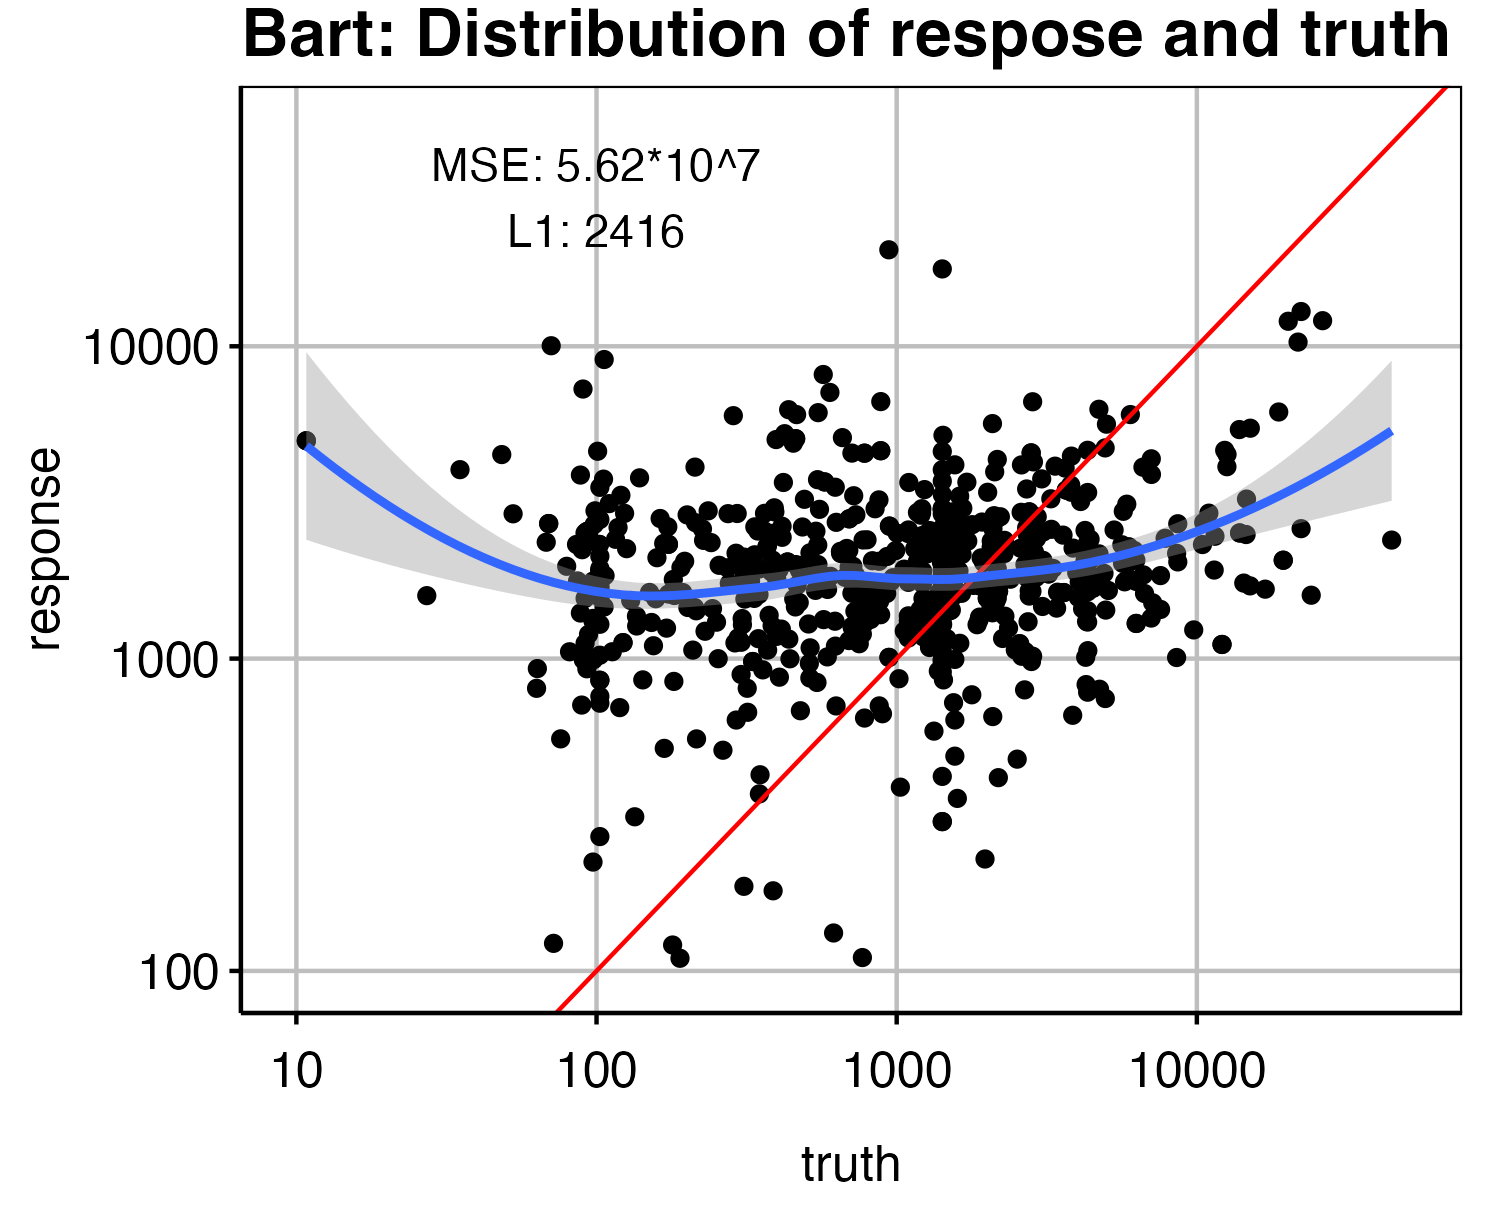
\includegraphics[width=0.34\textwidth]{figures/sev_p_bart_wide.png} }}
    \qquad
    \subfloat[\centering]{{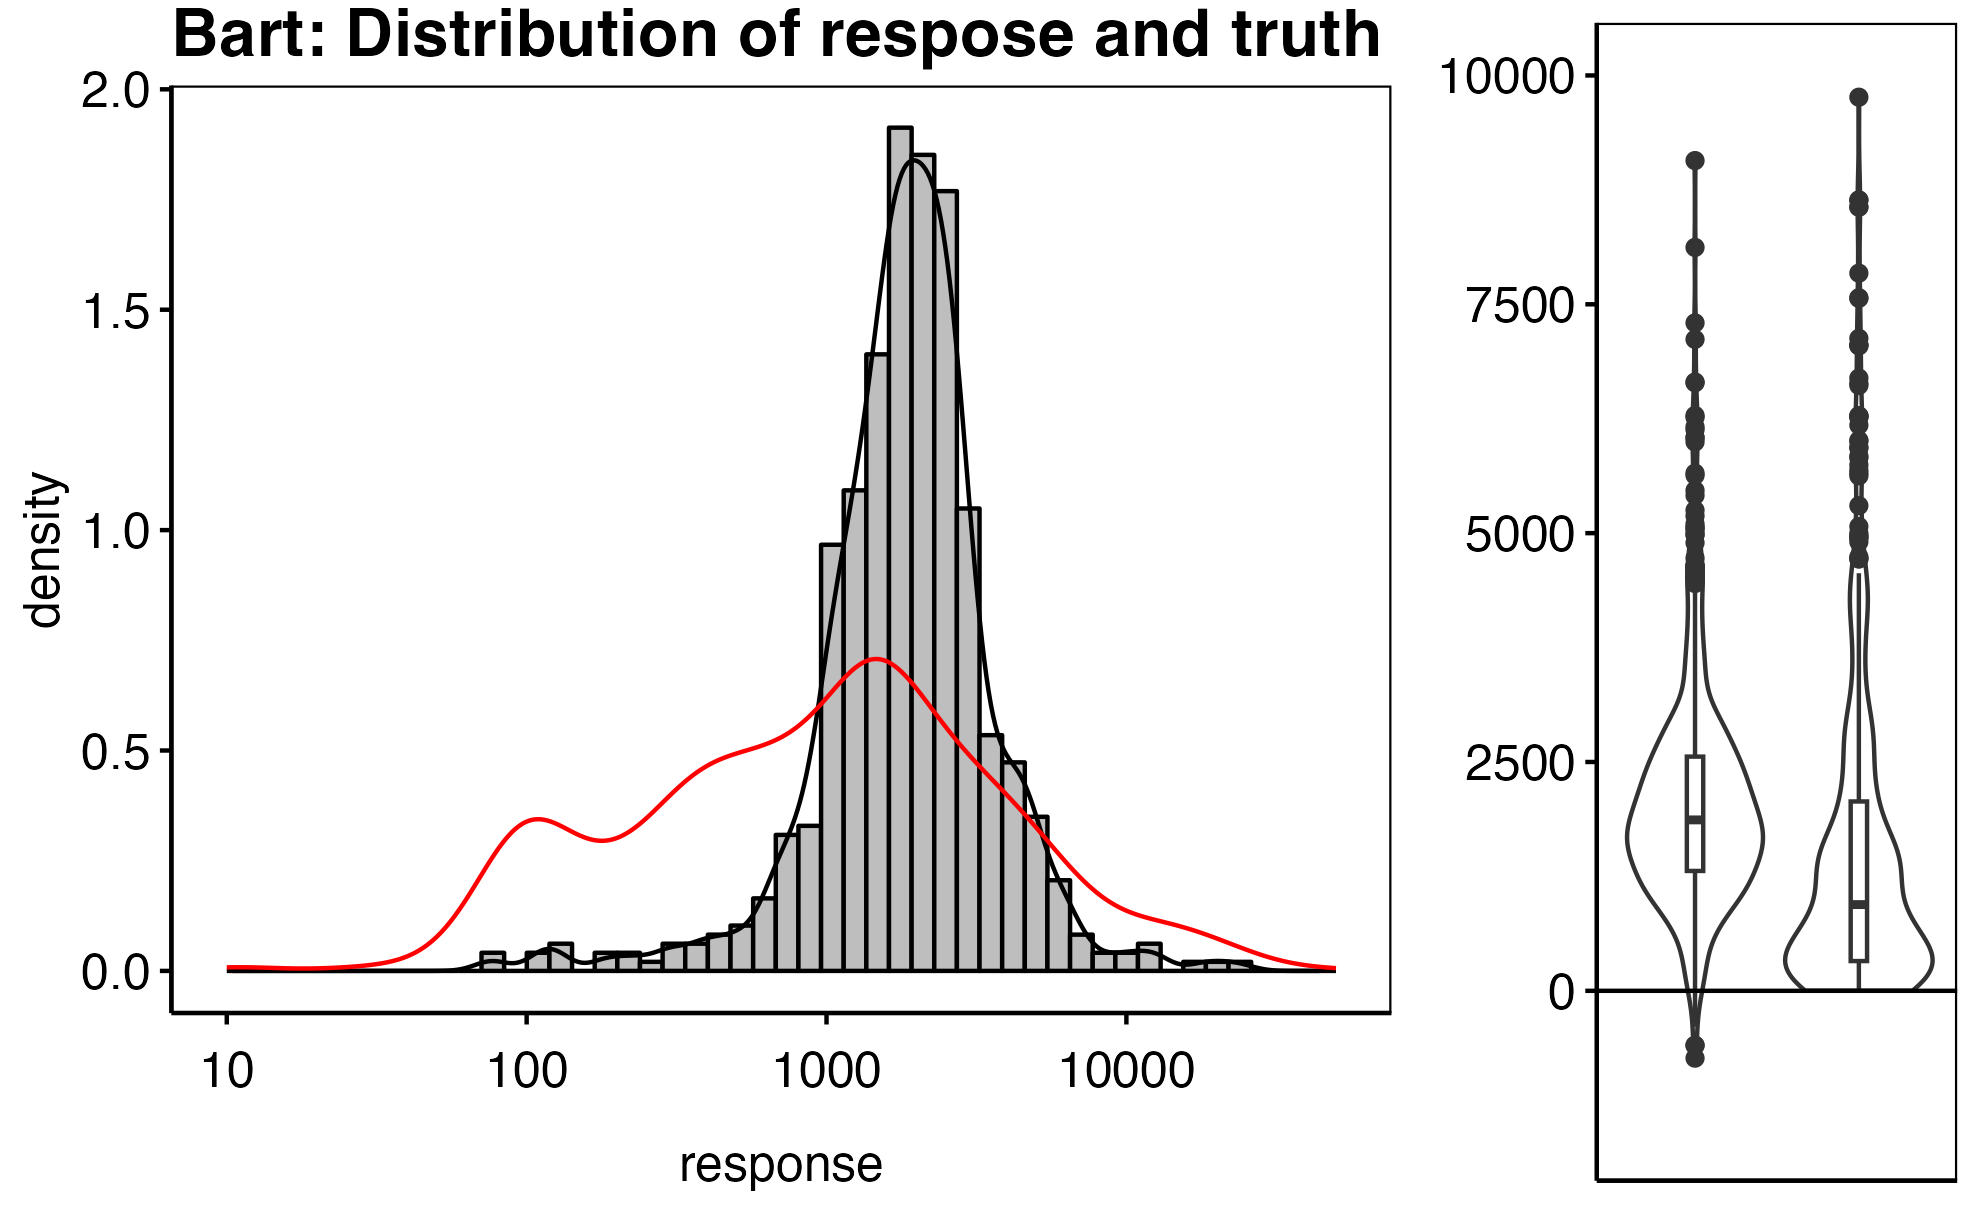
\includegraphics[width=0.46\textwidth]{figures/sev_p_bart3.png} }}
    \caption{(a): Predictions for the BART regression model with x being the actual value and y being the estimate. The red line represent the mapping $y=x$. (b, left): Distribution of the response and actual values. The red density function represents the empirical density of the test data set. (b, right): A combined boxplot and violin plot of the distribution of the response (left) and the actual value (right).}
\end{figure}

\begin{longtable}[]{@{}
  >{\centering\arraybackslash}p{(\columnwidth - 16\tabcolsep) * \real{0.1111}}
  >{\centering\arraybackslash}p{(\columnwidth - 16\tabcolsep) * \real{0.1111}}
  >{\centering\arraybackslash}p{(\columnwidth - 16\tabcolsep) * \real{0.1111}}
  >{\centering\arraybackslash}p{(\columnwidth - 16\tabcolsep) * \real{0.1111}}
  >{\centering\arraybackslash}p{(\columnwidth - 16\tabcolsep) * \real{0.1111}}
  >{\centering\arraybackslash}p{(\columnwidth - 16\tabcolsep) * \real{0.1111}}
  >{\centering\arraybackslash}p{(\columnwidth - 16\tabcolsep) * \real{0.1111}}
  >{\centering\arraybackslash}p{(\columnwidth - 16\tabcolsep) * \real{0.1111}}
  >{\centering\arraybackslash}p{(\columnwidth - 16\tabcolsep) * \real{0.1111}}@{}}
\toprule()
\begin{minipage}[b]{\linewidth}\centering
Estimator
\end{minipage} & \begin{minipage}[b]{\linewidth}\centering
\(\hat R_{L^2}\)
\end{minipage} & \begin{minipage}[b]{\linewidth}\centering
\(\hat R_{L^1}\)
\end{minipage} & \begin{minipage}[b]{\linewidth}\centering
6257
\end{minipage} & \begin{minipage}[b]{\linewidth}\centering
24131
\end{minipage} & \begin{minipage}[b]{\linewidth}\centering
25018
\end{minipage} & \begin{minipage}[b]{\linewidth}\centering
25196
\end{minipage} & \begin{minipage}[b]{\linewidth}\centering
30503
\end{minipage} & \begin{minipage}[b]{\linewidth}\centering
30563
\end{minipage} \\
\midrule()
\endhead
\(m^{(Bart)}_\mu\) & \(5.62\cdot 10^7\) & 2415.75 & 9366.62 & 3189.97 &
3488.9 & 2064.3 & 6641.56 & 1847.67 \\
\bottomrule()
\end{longtable}

\hypertarget{ranger}{%
\subsubsection{Ranger}\label{ranger}}

\begin{figure}[h]
    \centering
    \subfloat[\centering]{{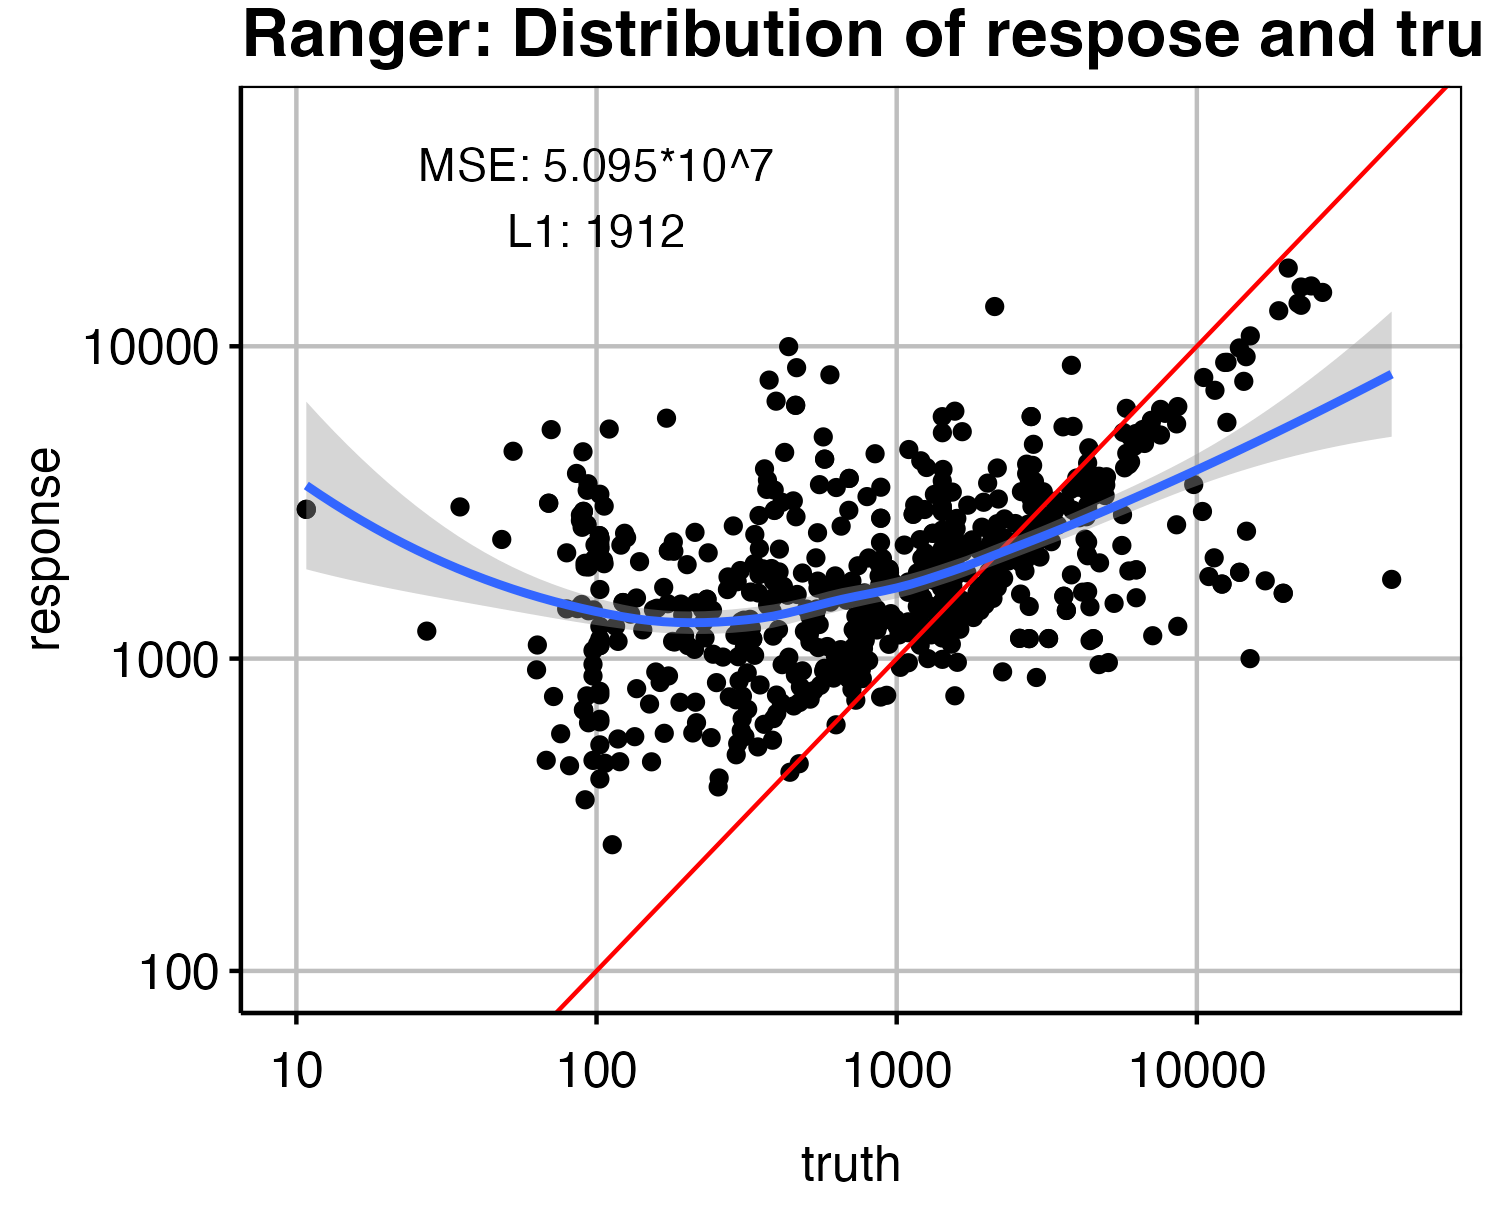
\includegraphics[width=0.34\textwidth]{figures/sev_p_ranger_wide.png} }}
    \qquad
    \subfloat[\centering]{{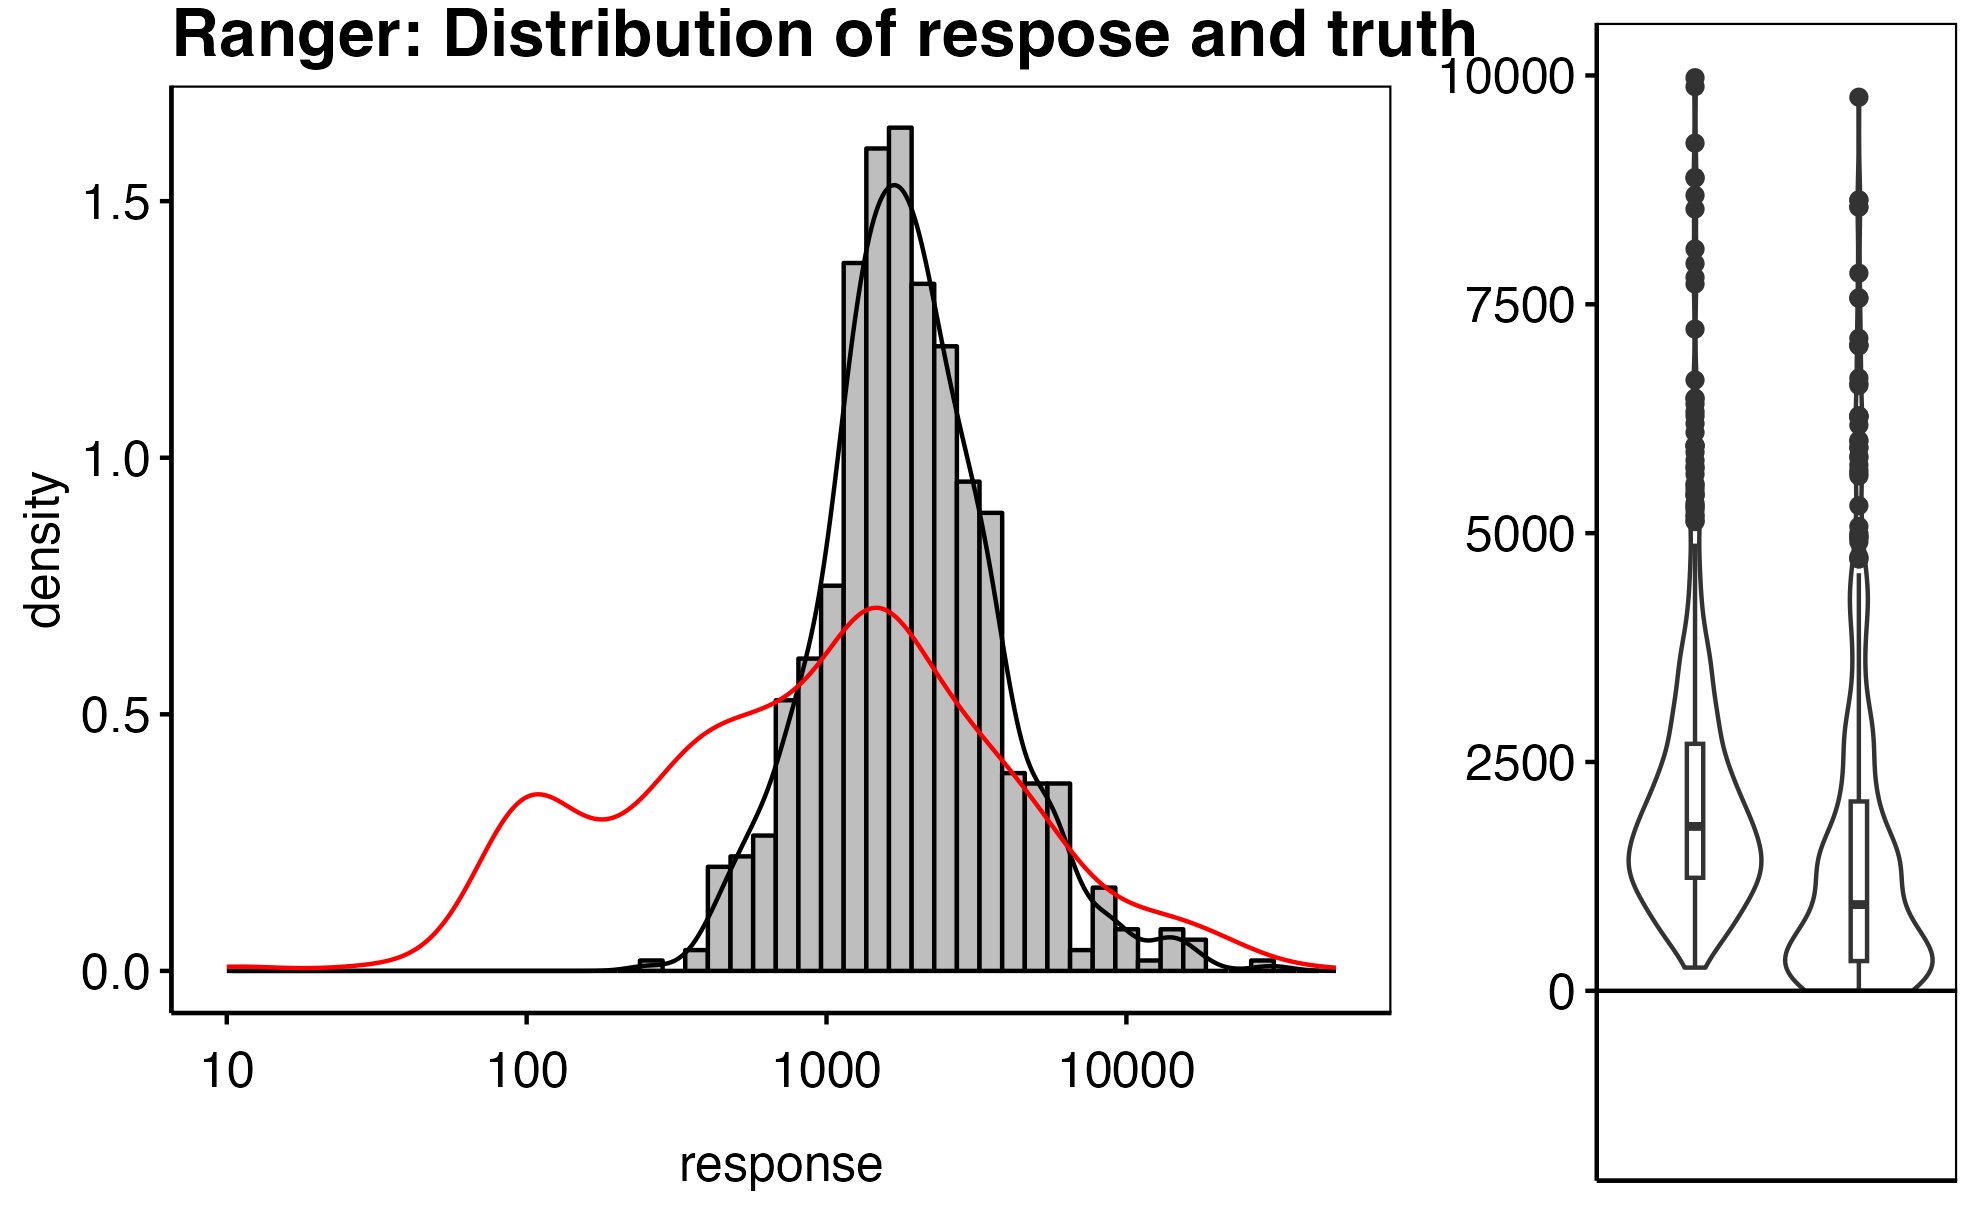
\includegraphics[width=0.46\textwidth]{figures/sev_p_ranger3.png} }}
    \caption{(a): Predictions for the ranger regression model with x being the actual value and y being the estimate. The red line represent the mapping $y=x$. (b, left): Distribution of the response and actual values. The red density function represents the empirical density of the test data set. (b, right): A combined boxplot and violin plot of the distribution of the response (left) and the actual value (right).}
\end{figure}

\begin{longtable}[]{@{}
  >{\centering\arraybackslash}p{(\columnwidth - 16\tabcolsep) * \real{0.1111}}
  >{\centering\arraybackslash}p{(\columnwidth - 16\tabcolsep) * \real{0.1111}}
  >{\centering\arraybackslash}p{(\columnwidth - 16\tabcolsep) * \real{0.1111}}
  >{\centering\arraybackslash}p{(\columnwidth - 16\tabcolsep) * \real{0.1111}}
  >{\centering\arraybackslash}p{(\columnwidth - 16\tabcolsep) * \real{0.1111}}
  >{\centering\arraybackslash}p{(\columnwidth - 16\tabcolsep) * \real{0.1111}}
  >{\centering\arraybackslash}p{(\columnwidth - 16\tabcolsep) * \real{0.1111}}
  >{\centering\arraybackslash}p{(\columnwidth - 16\tabcolsep) * \real{0.1111}}
  >{\centering\arraybackslash}p{(\columnwidth - 16\tabcolsep) * \real{0.1111}}@{}}
\toprule()
\begin{minipage}[b]{\linewidth}\centering
Estimator
\end{minipage} & \begin{minipage}[b]{\linewidth}\centering
\(\hat R_{L^2}\)
\end{minipage} & \begin{minipage}[b]{\linewidth}\centering
\(\hat R_{L^1}\)
\end{minipage} & \begin{minipage}[b]{\linewidth}\centering
6257
\end{minipage} & \begin{minipage}[b]{\linewidth}\centering
24131
\end{minipage} & \begin{minipage}[b]{\linewidth}\centering
25018
\end{minipage} & \begin{minipage}[b]{\linewidth}\centering
25196
\end{minipage} & \begin{minipage}[b]{\linewidth}\centering
30503
\end{minipage} & \begin{minipage}[b]{\linewidth}\centering
30563
\end{minipage} \\
\midrule()
\endhead
\(m^{(Ranger)}_\mu\) & \(5.095\cdot 10^7\) & 1912.16 & 10258.91 &
3956.79 & 5320.21 & 1683.94 & 4550.7 & 3248.58 \\
\bottomrule()
\end{longtable}

\newpage

\hypertarget{combining-results}{%
\subsubsection{Combining results}\label{combining-results}}

\begin{longtable}[]{@{}
  >{\raggedright\arraybackslash}p{(\columnwidth - 16\tabcolsep) * \real{0.0769}}
  >{\centering\arraybackslash}p{(\columnwidth - 16\tabcolsep) * \real{0.1154}}
  >{\centering\arraybackslash}p{(\columnwidth - 16\tabcolsep) * \real{0.1154}}
  >{\centering\arraybackslash}p{(\columnwidth - 16\tabcolsep) * \real{0.1154}}
  >{\centering\arraybackslash}p{(\columnwidth - 16\tabcolsep) * \real{0.1154}}
  >{\centering\arraybackslash}p{(\columnwidth - 16\tabcolsep) * \real{0.1154}}
  >{\centering\arraybackslash}p{(\columnwidth - 16\tabcolsep) * \real{0.1154}}
  >{\centering\arraybackslash}p{(\columnwidth - 16\tabcolsep) * \real{0.1154}}
  >{\centering\arraybackslash}p{(\columnwidth - 16\tabcolsep) * \real{0.1154}}@{}}
\toprule()
\begin{minipage}[b]{\linewidth}\raggedright
Estimator
\end{minipage} & \begin{minipage}[b]{\linewidth}\centering
\(\hat R_{L^2}\)
\end{minipage} & \begin{minipage}[b]{\linewidth}\centering
\(\hat R_{L^1}\)
\end{minipage} & \begin{minipage}[b]{\linewidth}\centering
6257
\end{minipage} & \begin{minipage}[b]{\linewidth}\centering
24131
\end{minipage} & \begin{minipage}[b]{\linewidth}\centering
25018
\end{minipage} & \begin{minipage}[b]{\linewidth}\centering
25196
\end{minipage} & \begin{minipage}[b]{\linewidth}\centering
30503
\end{minipage} & \begin{minipage}[b]{\linewidth}\centering
30563
\end{minipage} \\
\midrule()
\endhead
\(m^{(GAM)}_\mu\) & \(6.066\cdot 10^7\) & 2752.16 & 2463.49 & 4684.1 &
6047.67 & 2263.16 & 2009.47 & 1694.34 \\
\(m^{(EN)}_\mu\) & \(6.106\cdot 10^7\) & 2754.79 & 2338.48 & 1843.77 &
3206.72 & 2142.26 & 1143.72 & 1322.23 \\
\(m^{(XGB)}_\mu\) & \(5.916\cdot 10^7\) & 2357.03 & 4416.08 & 3226.21 &
6291.82 & 2634.91 & 3856.08 & 3239.16 \\
\(m^{(Bart)}_\mu\) & \(5.62\cdot 10^7\) & 2415.75 & 9366.62 & 3189.97 &
3488.9 & 2064.3 & 6641.56 & 1847.67 \\
\(m^{(Ranger)}_\mu\) & \(5.095\cdot 10^7\) & 1912.16 & 10258.91 &
3956.79 & 5320.21 & 1683.94 & 4550.7 & 3248.58 \\
\bottomrule()
\end{longtable}

We choose the Ranger model going forward because it has the lowest MLE
and it seems the most precise in estimating, seen on figure 9a. This is
maybe because random trees deal well with sparsity and thus the model
has worked around the high correlation of the variables.

The bad performance of the GAM model shows that the response might have
a very non-additive character which also speaks in favor of the Ranger
model since random trees deal very poorly with additive models.

\newpage

\hypertarget{modelling-frequency}{%
\subsection{Modelling frequency}\label{modelling-frequency}}

\begin{wrapfigure}{r}{0.50\textwidth}
  \begin{center}
    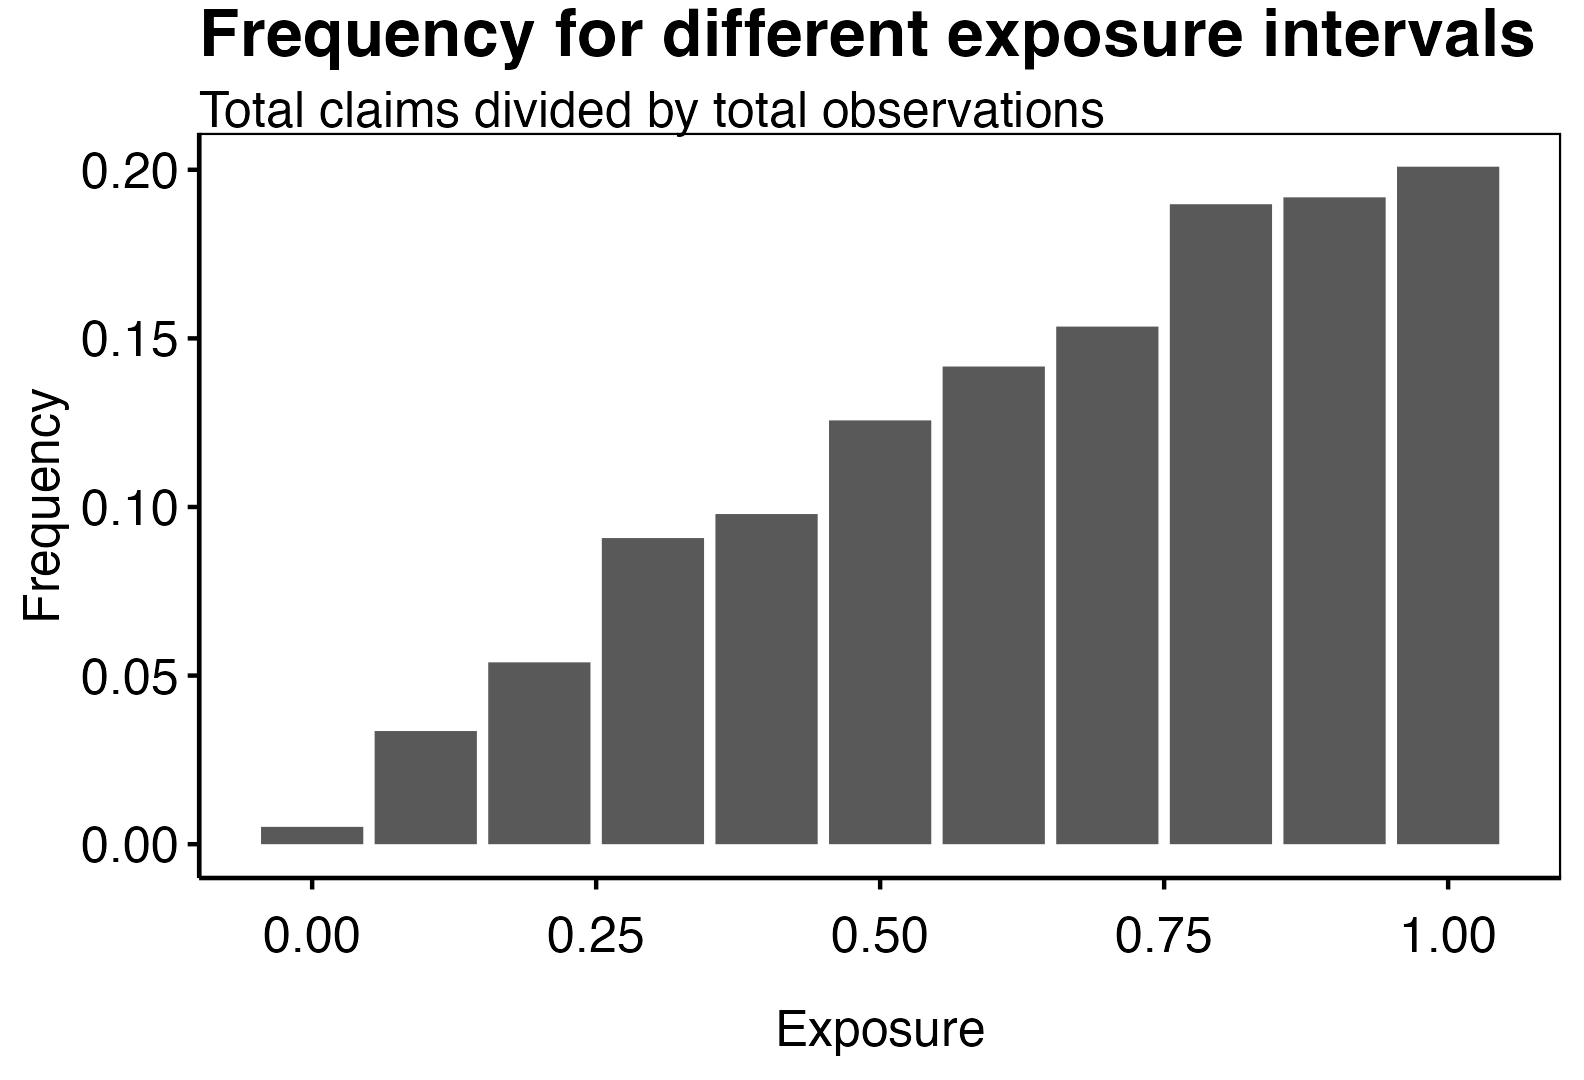
\includegraphics[width=0.48\textwidth]{figures/plot10.png}
  \end{center}
  \caption{The figure shows that the frequency is linear in exposure.}
\end{wrapfigure}

We have chosen to have exposure as an explanatory variable, since we
from the plots can see a somewhat linear tendency between the exposure
and Claimind. Thus the idea is that the more exposure you have the more
likelihood there is of you making a claim. We did not use the weight
method, because we do not want an observation with more exposure to have
a bigger impact, but rather that the risk is explained by the exposure.

When we evaluate the risk of the estimators we use the log loss function
given as

\[
L(y,p) = -\Big(y\cdot \log p + (1-y)\cdot \log(1-p)\Big).
\]

\hypertarget{generalized-additive-model-1}{%
\subsubsection{Generalized Additive
Model}\label{generalized-additive-model-1}}

We fit a Generalized additive model by fitting \texttt{ClaimInd} to the
covariates. Specifically this is done by choosing the logit link
function \(g\) in equation (1). The logit link function is given by

\[
g(p)=\log\left(\frac{p}{1-p}\right)=\log p-\log(1-p)\in \mathbb R.
\]

\begin{figure}[h]
    \centering
    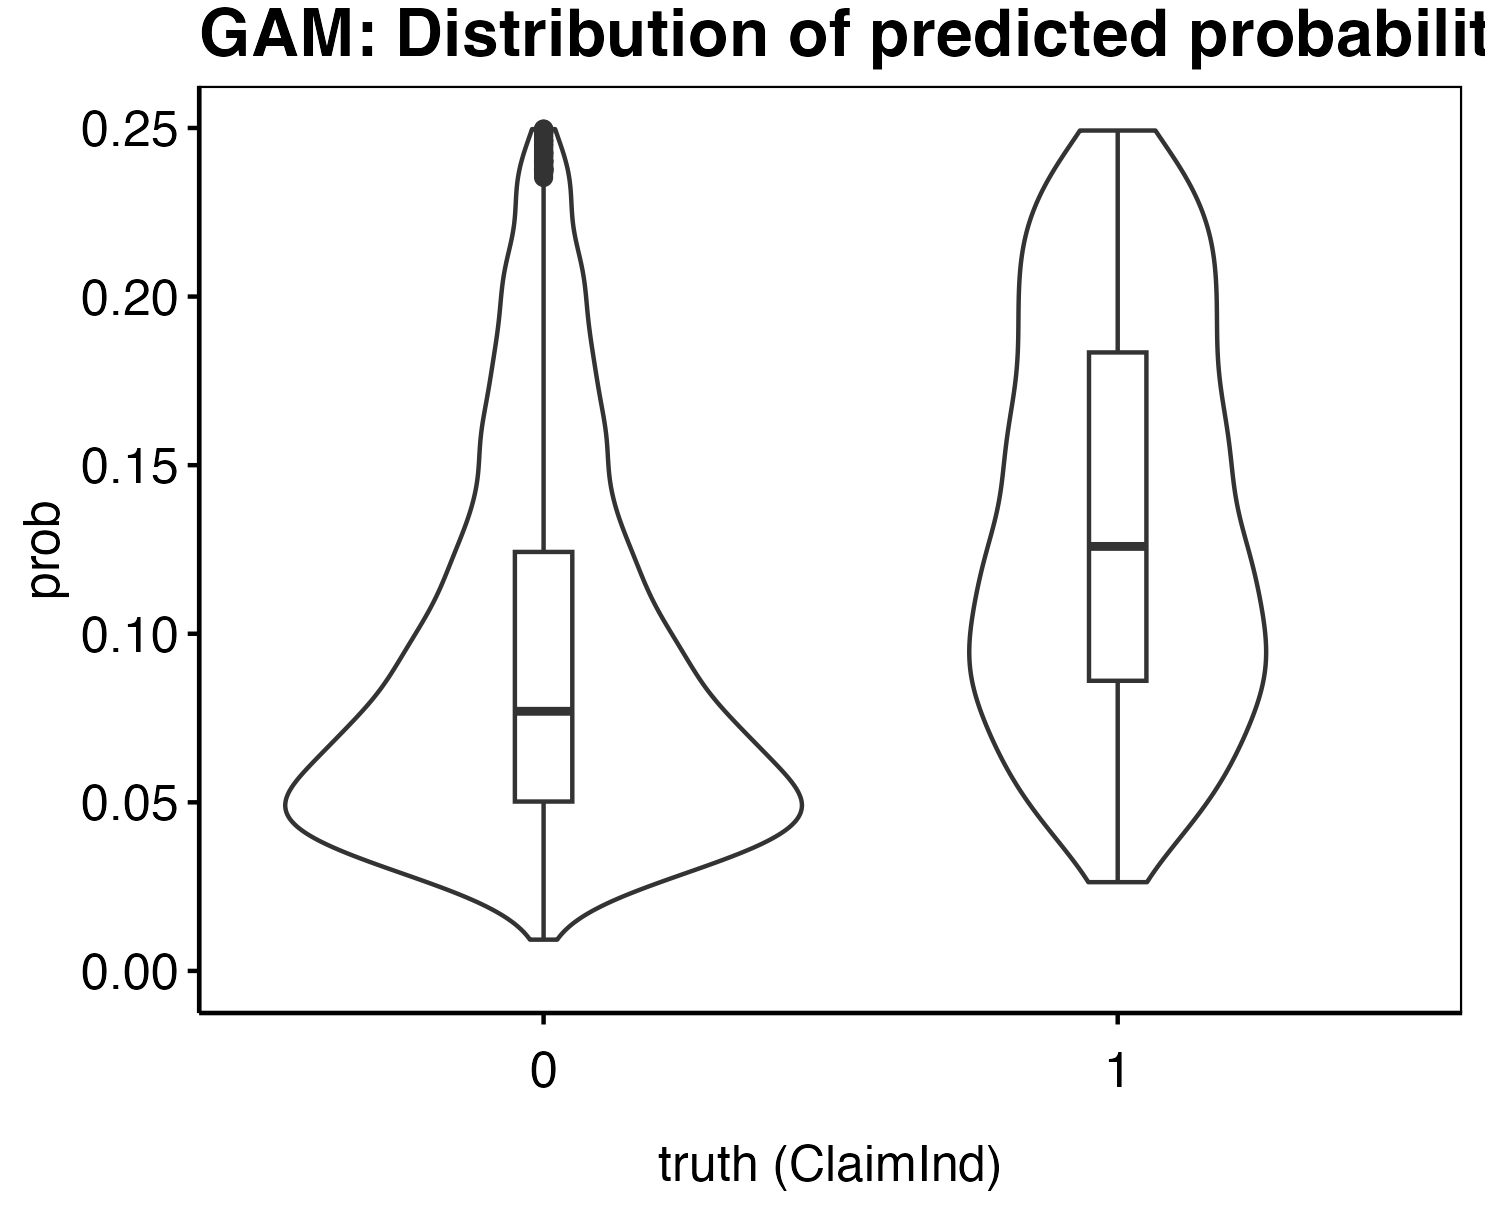
\includegraphics[width=0.34\textwidth]{figures/freq_p_gam_wide.png}
    \caption{A combined boxplot and violin plot of the distribution of the predicted probability for respectively the non claim (left) and claim (right) policies.}
\end{figure}

We can check the model predictions on a couple of specific policies,
namely the row numbers 6257, 25018, 30503 and 30563. Let us briefly take
a look at the four policies.

Then applying the estimator we obtain the estimates.

\begin{longtable}[]{@{}
  >{\centering\arraybackslash}p{(\columnwidth - 14\tabcolsep) * \real{0.1250}}
  >{\centering\arraybackslash}p{(\columnwidth - 14\tabcolsep) * \real{0.1250}}
  >{\centering\arraybackslash}p{(\columnwidth - 14\tabcolsep) * \real{0.1250}}
  >{\centering\arraybackslash}p{(\columnwidth - 14\tabcolsep) * \real{0.1250}}
  >{\centering\arraybackslash}p{(\columnwidth - 14\tabcolsep) * \real{0.1250}}
  >{\centering\arraybackslash}p{(\columnwidth - 14\tabcolsep) * \real{0.1250}}
  >{\centering\arraybackslash}p{(\columnwidth - 14\tabcolsep) * \real{0.1250}}
  >{\centering\arraybackslash}p{(\columnwidth - 14\tabcolsep) * \real{0.1250}}@{}}
\toprule()
\begin{minipage}[b]{\linewidth}\centering
Estimator
\end{minipage} & \begin{minipage}[b]{\linewidth}\centering
\(\hat R_{LL}\)
\end{minipage} & \begin{minipage}[b]{\linewidth}\centering
6257
\end{minipage} & \begin{minipage}[b]{\linewidth}\centering
24131
\end{minipage} & \begin{minipage}[b]{\linewidth}\centering
25018
\end{minipage} & \begin{minipage}[b]{\linewidth}\centering
25196
\end{minipage} & \begin{minipage}[b]{\linewidth}\centering
30503
\end{minipage} & \begin{minipage}[b]{\linewidth}\centering
30563
\end{minipage} \\
\midrule()
\endhead
\(m^{(GAM)}_p\) & 0.3142643 & 0.03748 & 0.0671 & 0.06536 & 0.03278 &
0.05206 & 0.08789 \\
\bottomrule()
\end{longtable}

\newpage

\hypertarget{elastic-net-linear-model-1}{%
\subsubsection{Elastic net linear
model}\label{elastic-net-linear-model-1}}

\begin{figure}[h]
    \centering
    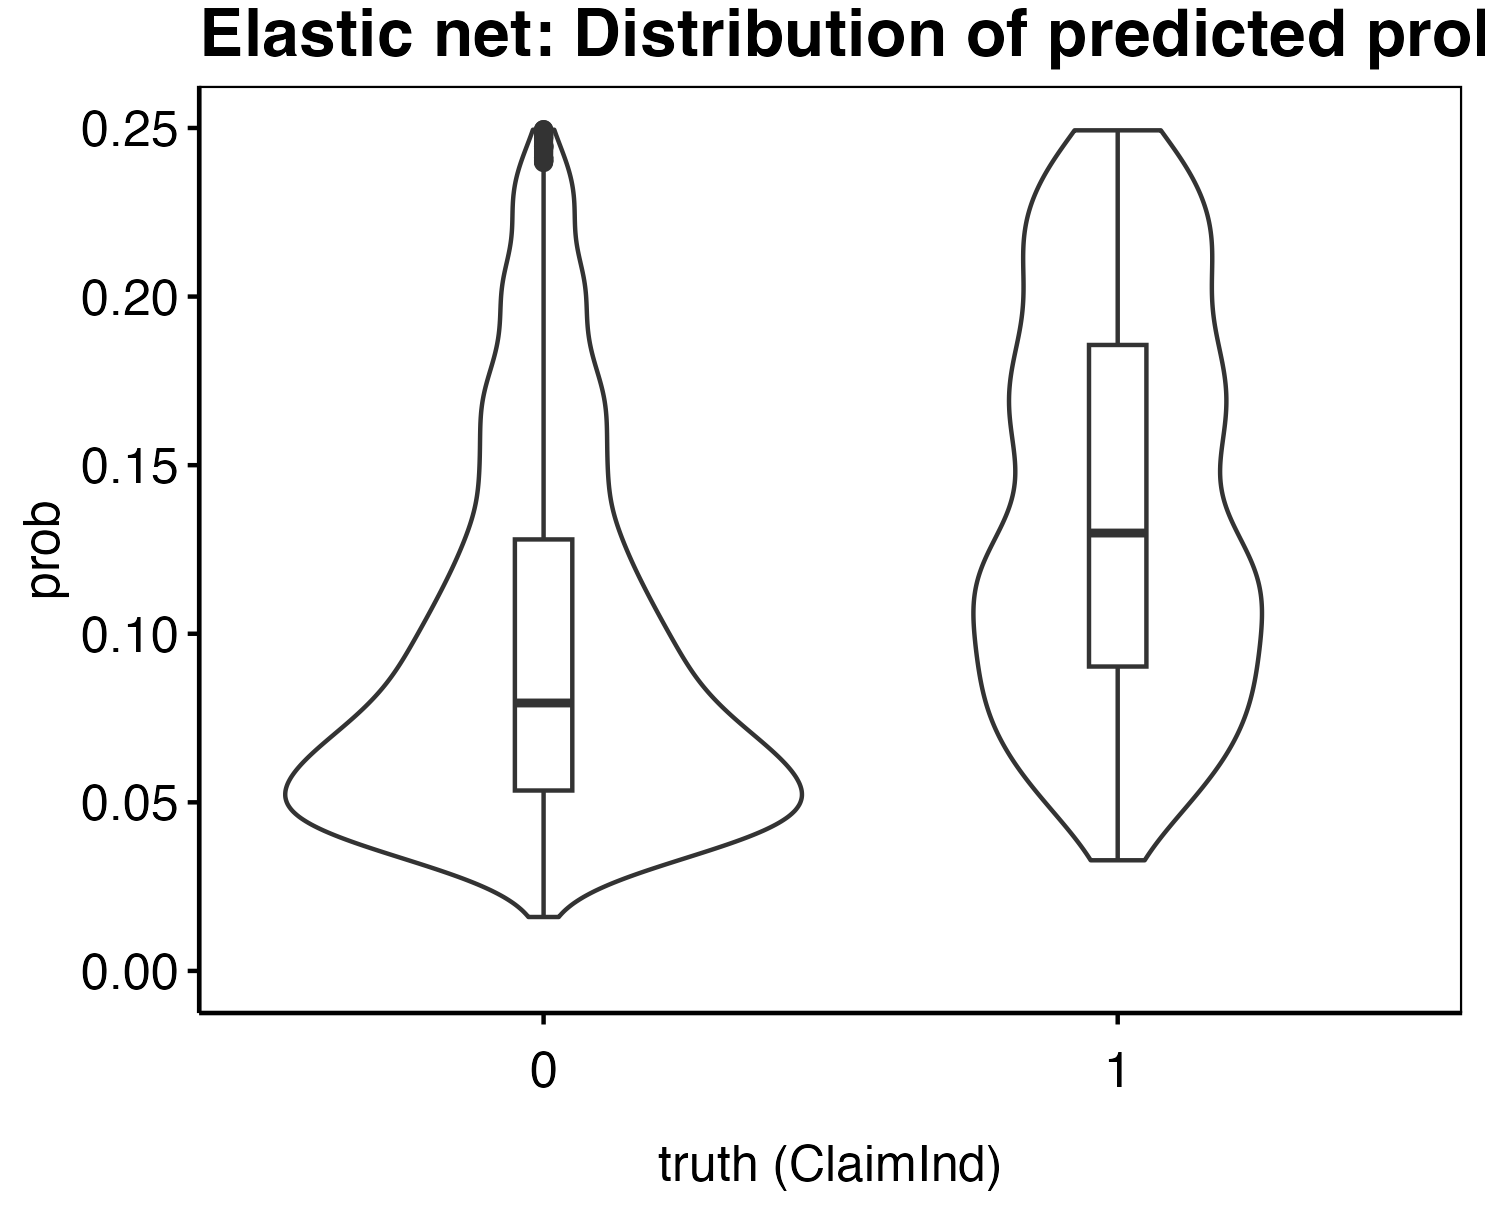
\includegraphics[width=0.34\textwidth]{figures/freq_p_glmnet_wide.png}
    \caption{A combined boxplot and violin plot of the distribution of the predicted probability for respectively the non claim (left) and claim (right) policies.}
\end{figure}

We can check the model predictions on a couple of specific policies,
namely the row numbers 6257, 25018, 30503 and 30563. Let us briefly take
a look at the four policies.

Then applying the estimator we obtain the estimates.

\begin{longtable}[]{@{}
  >{\centering\arraybackslash}p{(\columnwidth - 14\tabcolsep) * \real{0.1250}}
  >{\centering\arraybackslash}p{(\columnwidth - 14\tabcolsep) * \real{0.1250}}
  >{\centering\arraybackslash}p{(\columnwidth - 14\tabcolsep) * \real{0.1250}}
  >{\centering\arraybackslash}p{(\columnwidth - 14\tabcolsep) * \real{0.1250}}
  >{\centering\arraybackslash}p{(\columnwidth - 14\tabcolsep) * \real{0.1250}}
  >{\centering\arraybackslash}p{(\columnwidth - 14\tabcolsep) * \real{0.1250}}
  >{\centering\arraybackslash}p{(\columnwidth - 14\tabcolsep) * \real{0.1250}}
  >{\centering\arraybackslash}p{(\columnwidth - 14\tabcolsep) * \real{0.1250}}@{}}
\toprule()
\begin{minipage}[b]{\linewidth}\centering
Estimator
\end{minipage} & \begin{minipage}[b]{\linewidth}\centering
\(\hat R_{LL}\)
\end{minipage} & \begin{minipage}[b]{\linewidth}\centering
6257
\end{minipage} & \begin{minipage}[b]{\linewidth}\centering
24131
\end{minipage} & \begin{minipage}[b]{\linewidth}\centering
25018
\end{minipage} & \begin{minipage}[b]{\linewidth}\centering
25196
\end{minipage} & \begin{minipage}[b]{\linewidth}\centering
30503
\end{minipage} & \begin{minipage}[b]{\linewidth}\centering
30563
\end{minipage} \\
\midrule()
\endhead
\(m^{(EN)}_p\) & 0.3132799 & 0.04128 & 0.06164 & 0.06382 & 0.03882 &
0.03934 & 0.06055 \\
\bottomrule()
\end{longtable}

\hypertarget{xgboost-1}{%
\subsubsection{XGBoost}\label{xgboost-1}}

\begin{figure}[h]
    \centering
    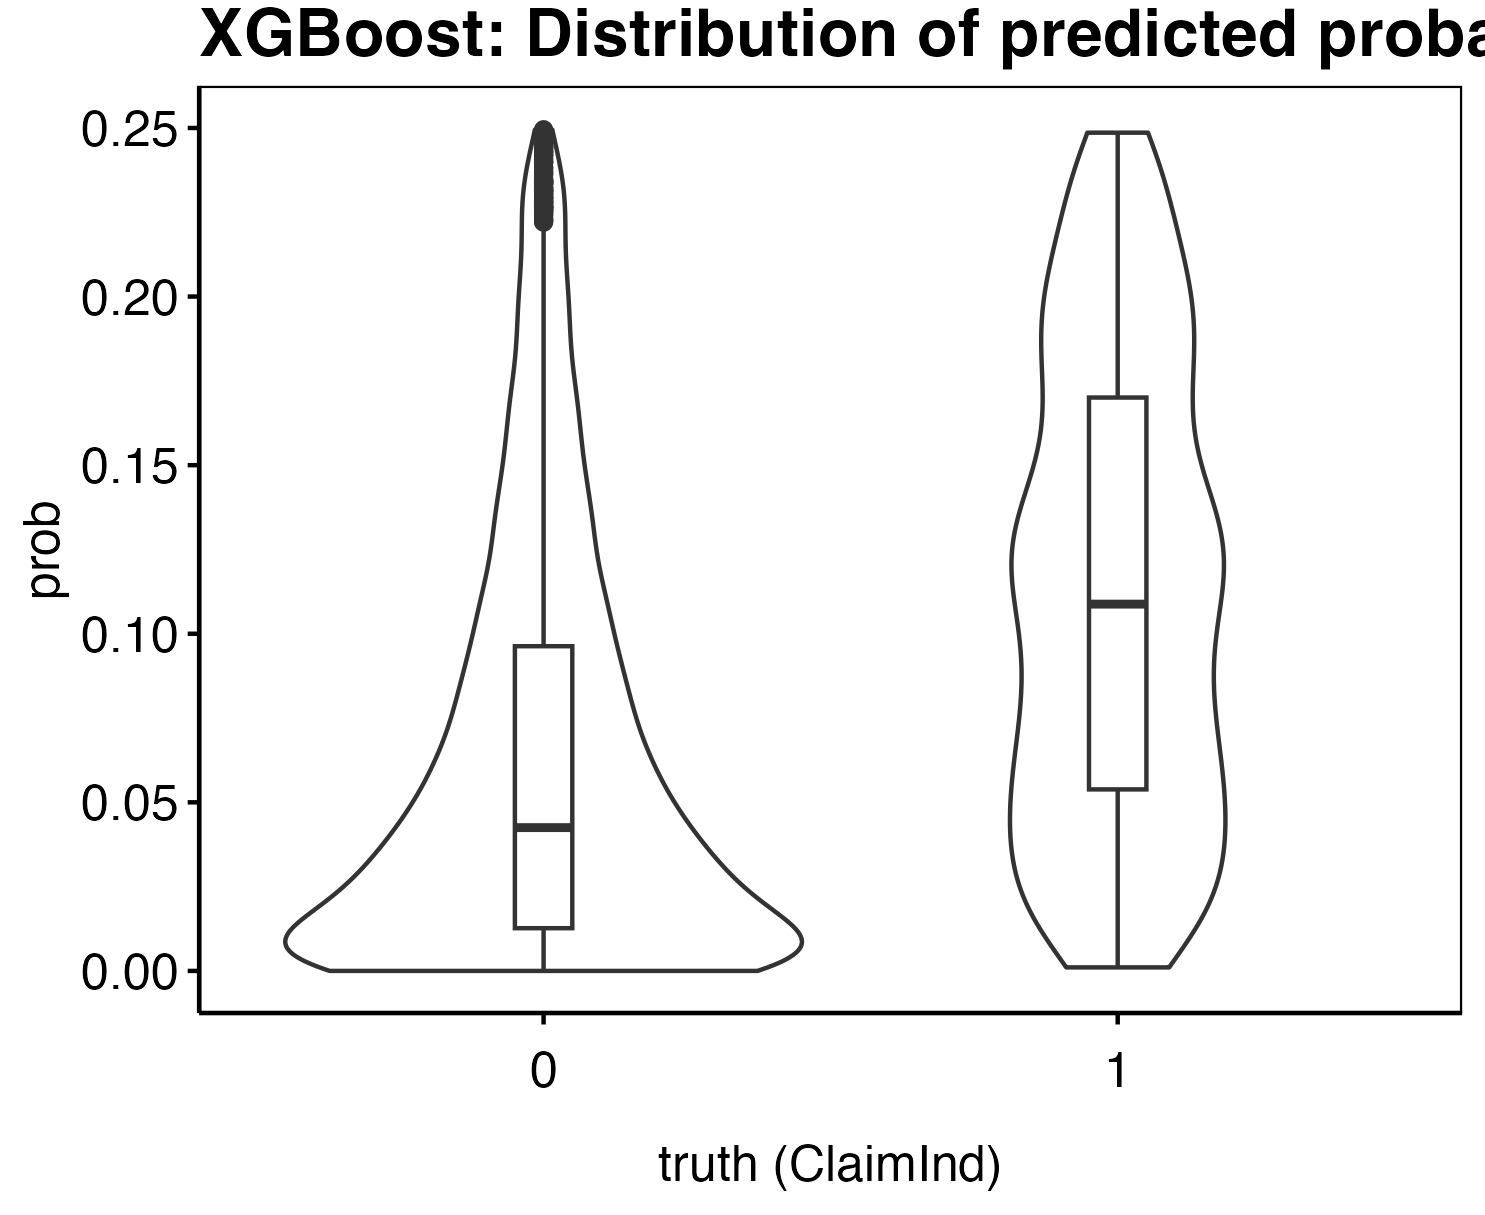
\includegraphics[width=0.34\textwidth]{figures/freq_p_xgb_wide.png}
    \caption{A combined boxplot and violin plot of the distribution of the predicted probability for respectively the non claim (left) and claim (right) policies.}
\end{figure}

We can check the model predictions on a couple of specific policies,
namely the row numbers 6257, 25018, 30503 and 30563. Let us briefly take
a look at the four policies.

Then applying the estimator we obtain the estimates.

\begin{longtable}[]{@{}
  >{\centering\arraybackslash}p{(\columnwidth - 14\tabcolsep) * \real{0.1250}}
  >{\centering\arraybackslash}p{(\columnwidth - 14\tabcolsep) * \real{0.1250}}
  >{\centering\arraybackslash}p{(\columnwidth - 14\tabcolsep) * \real{0.1250}}
  >{\centering\arraybackslash}p{(\columnwidth - 14\tabcolsep) * \real{0.1250}}
  >{\centering\arraybackslash}p{(\columnwidth - 14\tabcolsep) * \real{0.1250}}
  >{\centering\arraybackslash}p{(\columnwidth - 14\tabcolsep) * \real{0.1250}}
  >{\centering\arraybackslash}p{(\columnwidth - 14\tabcolsep) * \real{0.1250}}
  >{\centering\arraybackslash}p{(\columnwidth - 14\tabcolsep) * \real{0.1250}}@{}}
\toprule()
\begin{minipage}[b]{\linewidth}\centering
Estimator
\end{minipage} & \begin{minipage}[b]{\linewidth}\centering
\(\hat R_{LL}\)
\end{minipage} & \begin{minipage}[b]{\linewidth}\centering
6257
\end{minipage} & \begin{minipage}[b]{\linewidth}\centering
24131
\end{minipage} & \begin{minipage}[b]{\linewidth}\centering
25018
\end{minipage} & \begin{minipage}[b]{\linewidth}\centering
25196
\end{minipage} & \begin{minipage}[b]{\linewidth}\centering
30503
\end{minipage} & \begin{minipage}[b]{\linewidth}\centering
30563
\end{minipage} \\
\midrule()
\endhead
\(m^{(XGB)}_p\) & 0.2803893 & 0.01441 & 0.7285 & 0.30647 & 0.01226 &
0.00022 & 0.00174 \\
\bottomrule()
\end{longtable}

\hypertarget{bart-1}{%
\subsubsection{BART}\label{bart-1}}

\begin{figure}[h]
    \centering
    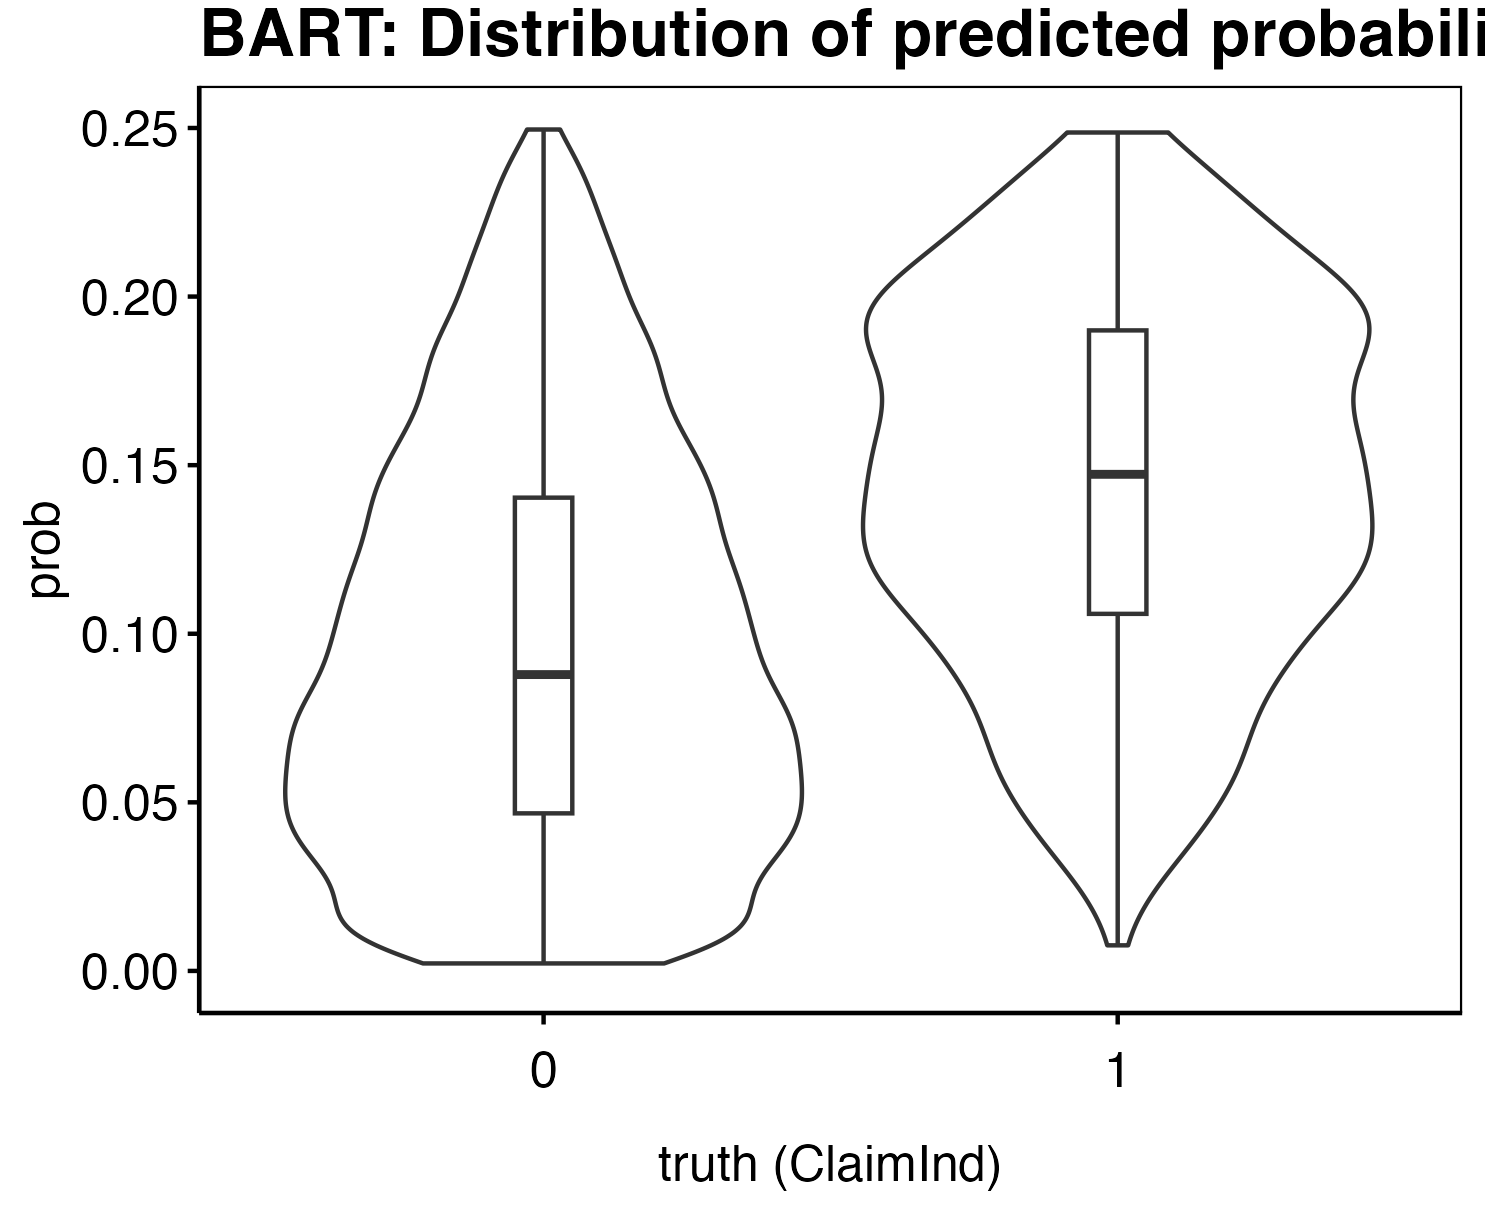
\includegraphics[width=0.34\textwidth]{figures/freq_p_bart_wide.png}
    \caption{A combined boxplot and violin plot of the distribution of the predicted probability for respectively the non claim (left) and claim (right) policies.}
\end{figure}

We can check the model predictions on a couple of specific policies,
namely the row numbers 6257, 25018, 30503 and 30563. Let us briefly take
a look at the four policies.

Then applying the estimator we obtain the estimates.

\begin{longtable}[]{@{}
  >{\centering\arraybackslash}p{(\columnwidth - 14\tabcolsep) * \real{0.1250}}
  >{\centering\arraybackslash}p{(\columnwidth - 14\tabcolsep) * \real{0.1250}}
  >{\centering\arraybackslash}p{(\columnwidth - 14\tabcolsep) * \real{0.1250}}
  >{\centering\arraybackslash}p{(\columnwidth - 14\tabcolsep) * \real{0.1250}}
  >{\centering\arraybackslash}p{(\columnwidth - 14\tabcolsep) * \real{0.1250}}
  >{\centering\arraybackslash}p{(\columnwidth - 14\tabcolsep) * \real{0.1250}}
  >{\centering\arraybackslash}p{(\columnwidth - 14\tabcolsep) * \real{0.1250}}
  >{\centering\arraybackslash}p{(\columnwidth - 14\tabcolsep) * \real{0.1250}}@{}}
\toprule()
\begin{minipage}[b]{\linewidth}\centering
Estimator
\end{minipage} & \begin{minipage}[b]{\linewidth}\centering
\(\hat R_{LL}\)
\end{minipage} & \begin{minipage}[b]{\linewidth}\centering
6257
\end{minipage} & \begin{minipage}[b]{\linewidth}\centering
24131
\end{minipage} & \begin{minipage}[b]{\linewidth}\centering
25018
\end{minipage} & \begin{minipage}[b]{\linewidth}\centering
25196
\end{minipage} & \begin{minipage}[b]{\linewidth}\centering
30503
\end{minipage} & \begin{minipage}[b]{\linewidth}\centering
30563
\end{minipage} \\
\midrule()
\endhead
\(m^{(Bart)}_p\) & 0.3093065 & 0.02454 & 0.07736 & 0.06091 & 0.02523 &
0.01419 & 0.09361 \\
\bottomrule()
\end{longtable}

\hypertarget{ranger-1}{%
\subsubsection{Ranger}\label{ranger-1}}

\begin{figure}[h]
    \centering
    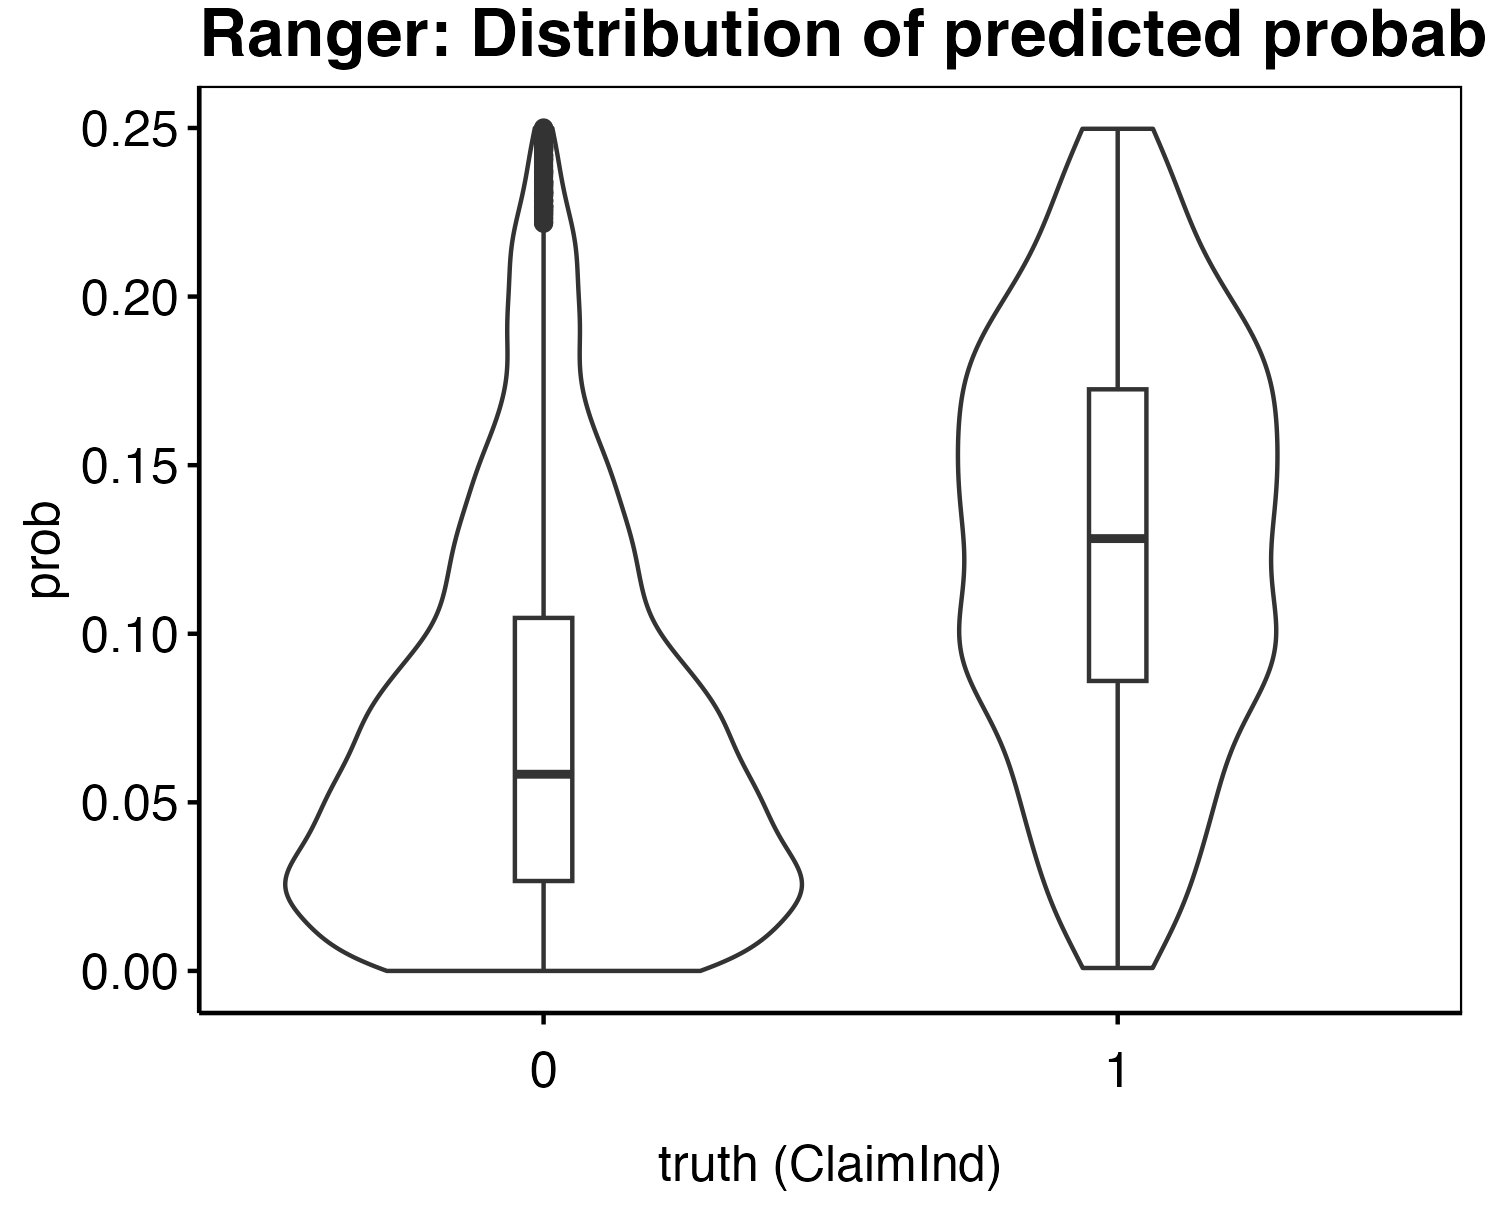
\includegraphics[width=0.34\textwidth]{figures/freq_p_ranger_wide.png}
    \caption{A combined boxplot and violin plot of the distribution of the predicted probability for respectively the non claim (left) and claim (right) policies.}
\end{figure}

We can check the model predictions on a couple of specific policies,
namely the row numbers 6257, 25018, 30503 and 30563. Let us briefly take
a look at the four policies.

Then applying the estimator we obtain the estimates.

\begin{longtable}[]{@{}
  >{\centering\arraybackslash}p{(\columnwidth - 14\tabcolsep) * \real{0.1250}}
  >{\centering\arraybackslash}p{(\columnwidth - 14\tabcolsep) * \real{0.1250}}
  >{\centering\arraybackslash}p{(\columnwidth - 14\tabcolsep) * \real{0.1250}}
  >{\centering\arraybackslash}p{(\columnwidth - 14\tabcolsep) * \real{0.1250}}
  >{\centering\arraybackslash}p{(\columnwidth - 14\tabcolsep) * \real{0.1250}}
  >{\centering\arraybackslash}p{(\columnwidth - 14\tabcolsep) * \real{0.1250}}
  >{\centering\arraybackslash}p{(\columnwidth - 14\tabcolsep) * \real{0.1250}}
  >{\centering\arraybackslash}p{(\columnwidth - 14\tabcolsep) * \real{0.1250}}@{}}
\toprule()
\begin{minipage}[b]{\linewidth}\centering
Estimator
\end{minipage} & \begin{minipage}[b]{\linewidth}\centering
\(\hat R_{LL}\)
\end{minipage} & \begin{minipage}[b]{\linewidth}\centering
6257
\end{minipage} & \begin{minipage}[b]{\linewidth}\centering
24131
\end{minipage} & \begin{minipage}[b]{\linewidth}\centering
25018
\end{minipage} & \begin{minipage}[b]{\linewidth}\centering
25196
\end{minipage} & \begin{minipage}[b]{\linewidth}\centering
30503
\end{minipage} & \begin{minipage}[b]{\linewidth}\centering
30563
\end{minipage} \\
\midrule()
\endhead
\(m^{(Ranger)}_p\) & 0.2260974 & 0 & 0.70167 & 0.34536 & 0.00667 &
0.08533 & 0.13714 \\
\bottomrule()
\end{longtable}

\newpage

\hypertarget{combining-results-1}{%
\subsubsection{Combining results}\label{combining-results-1}}

\begin{longtable}[]{@{}
  >{\centering\arraybackslash}p{(\columnwidth - 14\tabcolsep) * \real{0.1250}}
  >{\centering\arraybackslash}p{(\columnwidth - 14\tabcolsep) * \real{0.1250}}
  >{\centering\arraybackslash}p{(\columnwidth - 14\tabcolsep) * \real{0.1250}}
  >{\centering\arraybackslash}p{(\columnwidth - 14\tabcolsep) * \real{0.1250}}
  >{\centering\arraybackslash}p{(\columnwidth - 14\tabcolsep) * \real{0.1250}}
  >{\centering\arraybackslash}p{(\columnwidth - 14\tabcolsep) * \real{0.1250}}
  >{\centering\arraybackslash}p{(\columnwidth - 14\tabcolsep) * \real{0.1250}}
  >{\centering\arraybackslash}p{(\columnwidth - 14\tabcolsep) * \real{0.1250}}@{}}
\toprule()
\begin{minipage}[b]{\linewidth}\centering
Estimator
\end{minipage} & \begin{minipage}[b]{\linewidth}\centering
\(\hat R_{LL}\)
\end{minipage} & \begin{minipage}[b]{\linewidth}\centering
6257
\end{minipage} & \begin{minipage}[b]{\linewidth}\centering
24131
\end{minipage} & \begin{minipage}[b]{\linewidth}\centering
25018
\end{minipage} & \begin{minipage}[b]{\linewidth}\centering
25196
\end{minipage} & \begin{minipage}[b]{\linewidth}\centering
30503
\end{minipage} & \begin{minipage}[b]{\linewidth}\centering
30563
\end{minipage} \\
\midrule()
\endhead
\(m^{(GAM)}_p\) & 0.3142643 & 0.03748 & 0.0671 & 0.06536 & 0.03278 &
0.05206 & 0.08789 \\
\(m^{(EN)}_p\) & 0.3132799 & 0.04128 & 0.06164 & 0.06382 & 0.03882 &
0.03934 & 0.06055 \\
\(m^{(XGB)}_p\) & 0.2803893 & 0.01441 & 0.7285 & 0.30647 & 0.01226 &
0.00022 & 0.00174 \\
\(m^{(Bart)}_p\) & 0.3093065 & 0.02454 & 0.07736 & 0.06091 & 0.02523 &
0.01419 & 0.09361 \\
\(m^{(Ranger)}_p\) & 0.2260974 & 0 & 0.70167 & 0.34536 & 0.00667 &
0.08533 & 0.13714 \\
\bottomrule()
\end{longtable}

Once again the ranger model outperforms the other models. Furthermore,
it seems that the probabilities assign to the test data indicates, that
the estimator correctly assigns noteworthy larger probabilities to the
policies that indeed ended up with a claim. Lastly, one might want to
investigate if the model predicts probabilities very close to zero. If
so, we would maybe for business reasons rather penalize these
probabilities while transferring the increased income as savings to the
policies with a lower competitive price.

\newpage

\hypertarget{the-technical-price}{%
\subsection{The technical price}\label{the-technical-price}}

The technical price is given by the product

\[
\pi=\mu_X\cdot p_X.
\]

Notice that the length of the contract i.e.~the exposure is used as a
covariate in the frequency/severity model, and so the effect of longer
contracts is already priced in. By default new contracts are sold with a
yearly length, however in the case of estimating on the dataset we use
the given \texttt{Exposure}. Since the risk is the less with the ranger
algorithm we estimate \(\pi\) by

\[
\hat \pi=\hat m_\mu^{(Ranger)}(X)\cdot\hat m_p^{(Ranger)}(X)\cdot e.
\]

We can apply the technical price onto the dataset \texttt{freMPL1} by
running the following code:

\begin{Shaded}
\begin{Highlighting}[]
\CommentTok{\# Estimating mu}
\NormalTok{m\_mu\_ranger }\OtherTok{\textless{}{-}}\NormalTok{ sev\_ranger\_tuned\_regr}\SpecialCharTok{$}\FunctionTok{predict\_newdata}\NormalTok{(df)}\SpecialCharTok{$}\NormalTok{response}
\NormalTok{m\_mu\_ranger\_2 }\OtherTok{\textless{}{-}}\NormalTok{ df }\SpecialCharTok{\%\textgreater{}\%}
  \FunctionTok{mutate}\NormalTok{(}\AttributeTok{Exposure =} \DecValTok{1}\NormalTok{) }\SpecialCharTok{\%\textgreater{}\%}
\NormalTok{  sev\_ranger\_tuned\_regr}\SpecialCharTok{$}\FunctionTok{predict\_newdata}\NormalTok{(.)}
\NormalTok{m\_mu\_ranger\_2 }\OtherTok{\textless{}{-}}\NormalTok{ m\_mu\_ranger\_2}\SpecialCharTok{$}\NormalTok{response}
\CommentTok{\# Estimating p}
\NormalTok{m\_p\_ranger }\OtherTok{\textless{}{-}}\NormalTok{ freq\_ranger\_tuned}\SpecialCharTok{$}\FunctionTok{predict\_newdata}\NormalTok{(df\_freq)}\SpecialCharTok{$}\NormalTok{prob[,}\DecValTok{2}\NormalTok{]}
\NormalTok{m\_p\_ranger\_2 }\OtherTok{\textless{}{-}}\NormalTok{ df\_freq }\SpecialCharTok{\%\textgreater{}\%}
  \FunctionTok{mutate}\NormalTok{(}\AttributeTok{Exposure =} \DecValTok{1}\NormalTok{) }\SpecialCharTok{\%\textgreater{}\%}
\NormalTok{  freq\_ranger\_tuned}\SpecialCharTok{$}\FunctionTok{predict\_newdata}\NormalTok{(.)}
\NormalTok{m\_p\_ranger\_2 }\OtherTok{\textless{}{-}}\NormalTok{ m\_p\_ranger\_2}\SpecialCharTok{$}\NormalTok{prob[,}\DecValTok{2}\NormalTok{]}
\CommentTok{\# Inserting estimates}
\NormalTok{freMPL1[,}\StringTok{"pi\_hat"}\NormalTok{] }\OtherTok{\textless{}{-}}\NormalTok{ m\_mu\_ranger }\SpecialCharTok{*}\NormalTok{ m\_p\_ranger}
\NormalTok{freMPL1[,}\StringTok{"mu\_hat"}\NormalTok{] }\OtherTok{\textless{}{-}}\NormalTok{ m\_mu\_ranger}
\NormalTok{freMPL1[,}\StringTok{"p\_hat"}\NormalTok{] }\OtherTok{\textless{}{-}}\NormalTok{ m\_p\_ranger}
\NormalTok{freMPL1[,}\StringTok{"pi\_hat\_new"}\NormalTok{] }\OtherTok{\textless{}{-}}\NormalTok{ m\_mu\_ranger\_2 }\SpecialCharTok{*}\NormalTok{ m\_p\_ranger\_2}
\end{Highlighting}
\end{Shaded}

We can summarize the models predictions on the policies below.

\begin{longtable}[]{@{}cccccc@{}}
\toprule()
Policy & Exposure & \(\hat \mu_X\) & \(\hat p_X\) & \(\hat \pi\) & \\
\midrule()
\endhead
6257 & 0.08 & 10258.91 & 0 & 0 & \\
24131 & 0.2 & 3956.79 & 0.70167 & 2776.35 & \\
25018 & 0.1 & 5320.21 & 0.34536 & 1837.37 & \\
25196 & 0.08 & 1683.94 & 0.00667 & 11.23 & \\
30503 & 0.05 & 4550.7 & 0.08533 & 388.33 & \\
30563 & 0.41 & 3248.58 & 0.13714 & 445.51 & \\
\bottomrule()
\end{longtable}

If we set the exposure to one we get new estimates and the technical
price the insurance firm will give to new contracts.

\begin{longtable}[]{@{}cccccc@{}}
\toprule()
Policy & Exposure & \(\hat \mu_X\) & \(\hat p_X\) & \(\hat \pi\) & \\
\midrule()
\endhead
6257 & 1 & 10258.91 & 0.19805 & 2031.75 & \\
24131 & 1 & 3956.79 & 0.61167 & 2420.24 & \\
25018 & 1 & 5320.21 & 0.36131 & 1922.24 & \\
25196 & 1 & 1683.94 & 0.13167 & 221.72 & \\
30503 & 1 & 4550.7 & 0.24122 & 1097.73 & \\
30563 & 1 & 3248.58 & 0.23381 & 759.53 & \\
\bottomrule()
\end{longtable}

In the table above we have altered the dataset with exposure set to 1
for all rows, to predict the price of a new contract i.e.~with exposure
of one year. One sees that the prices for the new contracts are larger
than the technical price for the historical as the exposure is larger.
Furthermore as expected we see that the estimate \(\hat \mu_X\) does not
depend on the exposure.

\newpage

\hypertarget{repreducing-statement}{%
\section{Repreducing statement}\label{repreducing-statement}}

\hypertarget{packages}{%
\subsection{Packages}\label{packages}}

\begin{Shaded}
\begin{Highlighting}[]
\FunctionTok{library}\NormalTok{(CASdatasets)}
\FunctionTok{library}\NormalTok{(lattice) }
\FunctionTok{library}\NormalTok{(evmix)}
\FunctionTok{library}\NormalTok{(ggplot2)}
\FunctionTok{library}\NormalTok{(mlr3)}
\FunctionTok{library}\NormalTok{(mlr3learners)}
\FunctionTok{library}\NormalTok{(mlr3extralearners)}
\FunctionTok{library}\NormalTok{(dbarts)}
\FunctionTok{library}\NormalTok{(mlr3mbo)}
\FunctionTok{library}\NormalTok{(mlr3measures)}
\FunctionTok{library}\NormalTok{(mlr3tuning)}
\FunctionTok{library}\NormalTok{(ranger)}
\FunctionTok{library}\NormalTok{(mlr3viz)}
\FunctionTok{library}\NormalTok{(fastDummies)}
\FunctionTok{library}\NormalTok{(dplyr)}
\end{Highlighting}
\end{Shaded}

\hypertarget{statistical-data}{%
\subsection{Statistical data}\label{statistical-data}}

The data we will be working with is the \texttt{freMPL1} (\emph{French
Motor Personal Line datasets}) dataset from the package
\texttt{CASdatasets} (\emph{Computational Actuarial Science datasets}).
The author write the following regarding the dataset

\begin{quote}
This collection of ten datasets comes from a private motor French
insurer. Each dataset includes risk features, claim amount and claim
history of around 30,000 policies for year 2004.
\end{quote}

A detailed description of the variables may be read in the below table.

\begin{longtable}[]{@{}
  >{\raggedright\arraybackslash}p{(\columnwidth - 2\tabcolsep) * \real{0.4211}}
  >{\raggedright\arraybackslash}p{(\columnwidth - 2\tabcolsep) * \real{0.5789}}@{}}
\toprule()
\begin{minipage}[b]{\linewidth}\raggedright
Variable
\end{minipage} & \begin{minipage}[b]{\linewidth}\raggedright
Description
\end{minipage} \\
\midrule()
\endhead
\emph{Exposure} & The exposure, in years. \\
\emph{LicAge} & The driving licence age, in months. \\
\emph{RecordBeg} & Beginning date of record. \\
\emph{RecordEnd} & End date of record. \\
\emph{VehAge} & The vehicle age, in years. \\
\emph{Gender} & The gender, either ``Male'' or ``Female''. \\
\emph{MariStat} & The marital status, either ``Alone'' or ``Other''. \\
\emph{SocioCateg} & The social category known as CSP in France, between
``CSP1'' and ``CSP99''. \\
\emph{VehUsage} & The vehicle usage among ``Private'', ``Private+trip to
office'' ``Professional'', ``Professional run''. \\
\emph{DrivAge} & The driver age, in years (in France, people can drive a
car at 18). \\
\emph{HasKmLimit} & A numeric, 1 if there is a km limit for the policy,
0 otherwise. \\
\emph{BonusMalus} & A numeric for the bonus/malus, between 50 and 350:
\textless100 means bonus, \textgreater100 means malus in France. \\
\emph{VehBody} & The vehicle body, among
``bus'',``cabriolet'',``coupe'',``microvan'',``othermicrovan'', \\
\emph{VehPrice} & The category of the vehicle price from ``A''
(cheapest) to ``Z'' (most expensive). \\
\emph{VehEngine} & The vehicle engine, among
``carburation'',``directinjectionoverpowered'',``electric'', ``GPL'',
``injection'', ``injection overpowered''. \\
\emph{VehEnergy} & The vehicle energy, among ``diesel'', ``eletric'',
``GPL'', ``regular''. \\
\emph{VehMaxSpeed} & The VehMaxSpeed, among
``1-130km/h'',``130-140km/h'',``140-150km/h'',``150-160 km/h'',
``160-170 km/h'', ``170-180 km/h'', ``180-190 km/h'', ``190-200 km/h'',
``200-220 km/h'', ``220+ km/h''. \\
\emph{VehClass} & The vehicle class (unknown categories), among ``0'',
``A'', ``B'', ``H'', ``M1'', ``M2''. \\
\emph{ClaimAmount} & Total claim amount of the guarantee. \\
\emph{RiskVar} & Unkonw risk variable between 1 and 20, possibly
ordered. \\
\emph{Garage} & The garage, if any, among ``Collective garage'',
``None'', ``Private garage''. \\
\emph{ClaimInd} & Claim indicator of the guarantee. (this is not the
claim number) \\
\bottomrule()
\end{longtable}

\hypertarget{feature-formatting}{%
\subsubsection{Feature formatting}\label{feature-formatting}}

The following changes has been made to the data \texttt{freMPL1}:

\begin{enumerate}
\def\labelenumi{\arabic{enumi}.}
\tightlist
\item
  The columns \texttt{RecordBeg} and \texttt{RecordEnd} are discarded.
\item
  The negative \texttt{ClaimAmount} entries is overwritten with zeroes
  and the \texttt{ClaimIndicator} is changed accordingly.
\item
  The observations \texttt{VehEngine} being equal to either
  \texttt{electric} or \texttt{GPL} is removed.
\item
  The levels A-C, R-T and U-Z are combined in \texttt{VehPrice}.
\item
  The lowest two \texttt{VehMaxSpeed} are combined.
\item
  The category \texttt{bus} is layed under \texttt{sedan} in the column
  \texttt{VehBody}.
\item
  The \texttt{gender} column is also discarded.
\item
  The column \texttt{SocioCateg} is combined into three layers:
  \texttt{A}, \texttt{B} and \texttt{C}.
\end{enumerate}

These changes may be read in the script below.

\begin{Shaded}
\begin{Highlighting}[]
\DocumentationTok{\#\# Feature selection and formatting}
\FunctionTok{data}\NormalTok{(}\StringTok{"freMPL1"}\NormalTok{,}\AttributeTok{package =} \StringTok{"CASdatasets"}\NormalTok{)}
\CommentTok{\#Add id}
\NormalTok{freMPL1[,}\StringTok{"id"}\NormalTok{] }\OtherTok{\textless{}{-}} \DecValTok{1}\SpecialCharTok{:}\FunctionTok{dim}\NormalTok{(freMPL1)[}\DecValTok{1}\NormalTok{]}

\CommentTok{\#1: RecordBeg and RecordEnd discarded}
\NormalTok{freMPL1 }\OtherTok{\textless{}{-}}\NormalTok{ freMPL1 }\SpecialCharTok{\%\textgreater{}\%}
  \FunctionTok{select}\NormalTok{(}\SpecialCharTok{{-}}\NormalTok{RecordBeg,}\SpecialCharTok{{-}}\NormalTok{RecordEnd)}

\CommentTok{\#2: Claim amount and indicator}
\NormalTok{freMPL1}\SpecialCharTok{$}\NormalTok{ClaimAmount[freMPL1}\SpecialCharTok{$}\NormalTok{ClaimAmount}\SpecialCharTok{\textless{}}\DecValTok{0}\NormalTok{] }\OtherTok{\textless{}{-}} \DecValTok{0}
\NormalTok{freMPL1}\SpecialCharTok{$}\NormalTok{ClaimInd }\OtherTok{\textless{}{-}} \FunctionTok{ifelse}\NormalTok{(freMPL1}\SpecialCharTok{$}\NormalTok{ClaimAmount}\SpecialCharTok{\textgreater{}}\DecValTok{0}\NormalTok{,}\DecValTok{1}\NormalTok{,}\DecValTok{0}\NormalTok{)}

\CommentTok{\#3: Electric or GPL vehicals}
\NormalTok{freMPL1 }\OtherTok{\textless{}{-}}\NormalTok{ freMPL1 }\SpecialCharTok{\%\textgreater{}\%}
  \FunctionTok{filter}\NormalTok{(}\SpecialCharTok{!}\NormalTok{(VehEngine }\SpecialCharTok{\%in\%} \FunctionTok{c}\NormalTok{(}\StringTok{"electric"}\NormalTok{,}\StringTok{"GPL"}\NormalTok{)))}

\CommentTok{\#4: Combining price categories}
\FunctionTok{levels}\NormalTok{(freMPL1}\SpecialCharTok{$}\NormalTok{VehPrice)[}\DecValTok{1}\SpecialCharTok{:}\DecValTok{3}\NormalTok{] }\OtherTok{\textless{}{-}} \StringTok{"A{-}C"}
\NormalTok{n }\OtherTok{\textless{}{-}} \FunctionTok{length}\NormalTok{(}\FunctionTok{levels}\NormalTok{(freMPL1}\SpecialCharTok{$}\NormalTok{VehPrice))}
\FunctionTok{levels}\NormalTok{(freMPL1}\SpecialCharTok{$}\NormalTok{VehPrice)[(n}\DecValTok{{-}5}\NormalTok{)}\SpecialCharTok{:}\NormalTok{n] }\OtherTok{\textless{}{-}} \StringTok{"U{-}Z"}
\NormalTok{n }\OtherTok{\textless{}{-}} \FunctionTok{length}\NormalTok{(}\FunctionTok{levels}\NormalTok{(freMPL1}\SpecialCharTok{$}\NormalTok{VehPrice))}
\FunctionTok{levels}\NormalTok{(freMPL1}\SpecialCharTok{$}\NormalTok{VehPrice)[(n}\DecValTok{{-}3}\NormalTok{)}\SpecialCharTok{:}\NormalTok{(n}\DecValTok{{-}1}\NormalTok{)] }\OtherTok{\textless{}{-}} \StringTok{"R{-}T"}

\CommentTok{\#5: Combining max speed levels}
\FunctionTok{levels}\NormalTok{(freMPL1}\SpecialCharTok{$}\NormalTok{VehMaxSpeed)[}\DecValTok{1}\SpecialCharTok{:}\DecValTok{2}\NormalTok{] }\OtherTok{\textless{}{-}} \StringTok{"1{-}140 kmh"}

\CommentTok{\#6: Bus set to sedan}
\FunctionTok{levels}\NormalTok{(freMPL1}\SpecialCharTok{$}\NormalTok{VehBody)[}\FunctionTok{levels}\NormalTok{(freMPL1}\SpecialCharTok{$}\NormalTok{VehBody) }\SpecialCharTok{==} \StringTok{"bus"}\NormalTok{] }\OtherTok{\textless{}{-}} \StringTok{"sedan"}

\CommentTok{\#7: Gender discarded}
\NormalTok{freMPL1 }\OtherTok{\textless{}{-}}\NormalTok{ freMPL1 }\SpecialCharTok{\%\textgreater{}\%}
  \FunctionTok{select}\NormalTok{(}\SpecialCharTok{{-}}\NormalTok{Gender)}

\CommentTok{\#8: SocioCateg change levels}
\NormalTok{freMPL1 }\OtherTok{\textless{}{-}}\NormalTok{ freMPL1 }\SpecialCharTok{\%\textgreater{}\%}
  \CommentTok{\#Get numerical value of SocioCateg}
  \FunctionTok{mutate}\NormalTok{(}\AttributeTok{helper =} \FunctionTok{as.numeric}\NormalTok{(}\FunctionTok{substr}\NormalTok{(SocioCateg,}\DecValTok{4}\NormalTok{,}\DecValTok{5}\NormalTok{))) }\SpecialCharTok{\%\textgreater{}\%}
  \CommentTok{\#Overwrite SocioCateg }
  \FunctionTok{mutate}\NormalTok{(}\AttributeTok{SocioCateg =} \FunctionTok{factor}\NormalTok{(}\FunctionTok{ifelse}\NormalTok{(helper }\SpecialCharTok{\textgreater{}} \DecValTok{50}\NormalTok{, }\StringTok{"C"}\NormalTok{,}
                                    \FunctionTok{ifelse}\NormalTok{( helper }\SpecialCharTok{\textless{}} \DecValTok{50}\NormalTok{, }\StringTok{"A"}\NormalTok{,}
                                            \StringTok{"B"}\NormalTok{)),}
                             \AttributeTok{levels =} \FunctionTok{c}\NormalTok{(}\StringTok{"A"}\NormalTok{,}\StringTok{"B"}\NormalTok{,}\StringTok{"C"}\NormalTok{))) }\SpecialCharTok{\%\textgreater{}\%}
  \FunctionTok{select}\NormalTok{(}\SpecialCharTok{{-}}\NormalTok{helper)}
\end{Highlighting}
\end{Shaded}

\hypertarget{preparing-the-dataset}{%
\subsubsection{Preparing the dataset}\label{preparing-the-dataset}}

We lastly format the data by creating a data frame called \texttt{data}
which we will henceforth be referring to. The data frame is created with
splitting the catagorical variables into indicators given whether or not
a covariates is equal to a given level. For instance the
\texttt{VehEnergy} column with the levels \texttt{diesel},
\texttt{eletric}, \texttt{GPL} and \texttt{regular} are split into the
columns \texttt{VehEnergy\_diesel}, \texttt{VehEnergy\_eletric},
\texttt{VehEnergy\_GPL} and \texttt{VehEnergy\_regular}, where per row
only one is equal to 1 and the rest equal to 0.

\begin{Shaded}
\begin{Highlighting}[]
\NormalTok{df }\OtherTok{\textless{}{-}}\NormalTok{ freMPL1 }\SpecialCharTok{\%\textgreater{}\%}
  \FunctionTok{dummy\_cols}\NormalTok{(.,}\AttributeTok{select\_columns =} \FunctionTok{c}\NormalTok{(}\StringTok{"VehAge"}\NormalTok{,}\StringTok{"MariStat"}\NormalTok{,}\StringTok{"VehUsage"}\NormalTok{,}
                                  \StringTok{"VehBody"}\NormalTok{,}\StringTok{"VehPrice"}\NormalTok{,}\StringTok{"VehEngine"}\NormalTok{,}
                                  \StringTok{"VehEnergy"}\NormalTok{,}\StringTok{"VehMaxSpeed"}\NormalTok{,}\StringTok{"VehClass"}\NormalTok{,}
                                  \StringTok{"Garage"}\NormalTok{,}\StringTok{"SocioCateg"}\NormalTok{,}\StringTok{"RiskVar"}\NormalTok{),}
             \AttributeTok{remove\_selected\_columns =} \ConstantTok{TRUE}\NormalTok{)}
\FunctionTok{colnames}\NormalTok{(df) }\OtherTok{\textless{}{-}} \FunctionTok{make.names}\NormalTok{(}\FunctionTok{colnames}\NormalTok{(df))}
\end{Highlighting}
\end{Shaded}

\hypertarget{severity-models}{%
\subsection{Severity models}\label{severity-models}}

\hypertarget{starting-a-task}{%
\subsubsection{Starting a task}\label{starting-a-task}}

We start by preparing test and training data and start a task.

\begin{Shaded}
\begin{Highlighting}[]
\CommentTok{\#Get the severity data}
\NormalTok{df\_sev }\OtherTok{\textless{}{-}}\NormalTok{ df }\SpecialCharTok{\%\textgreater{}\%} 
  \FunctionTok{filter}\NormalTok{(ClaimInd }\SpecialCharTok{==} \DecValTok{1}\NormalTok{) }\SpecialCharTok{\%\textgreater{}\%}
  \FunctionTok{select}\NormalTok{(}\SpecialCharTok{{-}}\NormalTok{Exposure,}\SpecialCharTok{{-}}\NormalTok{id)}

\CommentTok{\#Start a task}
\NormalTok{task\_sev }\OtherTok{\textless{}{-}}\NormalTok{ df\_sev }\SpecialCharTok{\%\textgreater{}\%}
  \CommentTok{\#Make sure not to include ClaimInd}
  \FunctionTok{select}\NormalTok{(}\SpecialCharTok{{-}}\NormalTok{ClaimInd) }\SpecialCharTok{\%\textgreater{}\%}
  \CommentTok{\#Start tast with target ClaimAmound}
  \FunctionTok{as\_task\_regr}\NormalTok{(.,}
               \AttributeTok{target =} \StringTok{"ClaimAmount"}\NormalTok{,}
               \AttributeTok{id=} \StringTok{"Severity"}\NormalTok{)}

\CommentTok{\#Split data into training and test}
\FunctionTok{set.seed}\NormalTok{(}\DecValTok{20230313}\NormalTok{) }\CommentTok{\#We choose a seed}
\NormalTok{splits }\OtherTok{\textless{}{-}} \FunctionTok{partition}\NormalTok{(task\_sev,}
                    \AttributeTok{ratio =} \FloatTok{0.8}\NormalTok{)}
\NormalTok{df\_sev\_train }\OtherTok{\textless{}{-}}\NormalTok{ df\_sev[splits}\SpecialCharTok{$}\NormalTok{train,]}
\NormalTok{df\_sev\_test }\OtherTok{\textless{}{-}}\NormalTok{ df\_sev[splits}\SpecialCharTok{$}\NormalTok{test,]}

\CommentTok{\#Start task on training data}
\NormalTok{task\_sev\_train }\OtherTok{\textless{}{-}} \FunctionTok{as\_task\_regr}\NormalTok{(df\_sev\_train, }\AttributeTok{target =} \StringTok{"ClaimAmount"}\NormalTok{)}
\end{Highlighting}
\end{Shaded}

\hypertarget{defining-learners}{%
\subsubsection{Defining learners}\label{defining-learners}}

Now we define a learner for each of the five estimators some will be
tuned in the following section.

\begin{Shaded}
\begin{Highlighting}[]
\DocumentationTok{\#\#\# Generalized Additive Model}
\NormalTok{sev\_gam\_tuned\_regr }\OtherTok{\textless{}{-}} \FunctionTok{lrn}\NormalTok{(}\StringTok{"regr.gam"}\NormalTok{) }
\NormalTok{indicators }\OtherTok{\textless{}{-}} \FunctionTok{colnames}\NormalTok{(df)[}\SpecialCharTok{!}\NormalTok{(}\FunctionTok{colnames}\NormalTok{(df) }\SpecialCharTok{\%in\%} \FunctionTok{c}\NormalTok{(}\StringTok{"LicAge"}\NormalTok{,}\StringTok{"BonusMalus"}\NormalTok{,}
                                                 \StringTok{"DrivAge"}\NormalTok{,}\StringTok{"ClaimAmount"}\NormalTok{,}
                                                 \StringTok{"Exposure"}\NormalTok{,}\StringTok{"ClaimInd"}\NormalTok{,}\StringTok{"id"}\NormalTok{))]}
\NormalTok{sev\_gam\_tuned\_regr}\SpecialCharTok{$}\NormalTok{param\_set}\SpecialCharTok{$}\NormalTok{values}\SpecialCharTok{$}\NormalTok{formula }\OtherTok{\textless{}{-}} \FunctionTok{reformulate}\NormalTok{(}\FunctionTok{c}\NormalTok{(}\StringTok{"s(LicAge)"}\NormalTok{,}
                                                         \StringTok{"s(BonusMalus)"}\NormalTok{,}
                                                         \StringTok{"s(DrivAge)"}\NormalTok{,}
\NormalTok{                                                         indicators),}
                                                       \StringTok{"ClaimAmount"}\NormalTok{)}
\DocumentationTok{\#\#\# Elastic net}
\NormalTok{sev\_glmnet\_learner }\OtherTok{\textless{}{-}} \FunctionTok{lrn}\NormalTok{(}\StringTok{"regr.glmnet"}\NormalTok{, }
                        \AttributeTok{s=} \FunctionTok{to\_tune}\NormalTok{(}\DecValTok{0}\NormalTok{, }\DecValTok{1}\NormalTok{),}
                        \AttributeTok{alpha=}\FunctionTok{to\_tune}\NormalTok{(}\DecValTok{0}\NormalTok{, }\DecValTok{1}\NormalTok{))}

\DocumentationTok{\#\#\# XGBoost}
\NormalTok{sev\_xgb\_learner }\OtherTok{\textless{}{-}} \FunctionTok{lrn}\NormalTok{(}\StringTok{"regr.xgboost"}\NormalTok{, }
                   \AttributeTok{eta =} \FunctionTok{to\_tune}\NormalTok{(}\DecValTok{0}\NormalTok{, }\FloatTok{0.5}\NormalTok{),}
                   \AttributeTok{nrounds =} \FunctionTok{to\_tune}\NormalTok{(}\DecValTok{10}\NormalTok{, }\DecValTok{5000}\NormalTok{),}
                   \AttributeTok{max\_depth =} \FunctionTok{to\_tune}\NormalTok{(}\DecValTok{1}\NormalTok{, }\DecValTok{3}\NormalTok{))}

\DocumentationTok{\#\#\# BART}
\NormalTok{sev\_bart\_learner }\OtherTok{\textless{}{-}} \FunctionTok{lrn}\NormalTok{(}\StringTok{"regr.bart"}\NormalTok{,}
                        \AttributeTok{ntree =} \FunctionTok{to\_tune}\NormalTok{(}\DecValTok{73}\NormalTok{,}\DecValTok{400}\NormalTok{))}

\DocumentationTok{\#\#\# RANGER}
\NormalTok{sev\_ranger\_learner }\OtherTok{\textless{}{-}} \FunctionTok{lrn}\NormalTok{(}\StringTok{"regr.ranger"}\NormalTok{, }
                      \AttributeTok{mtry.ratio =} \FunctionTok{to\_tune}\NormalTok{(}\FloatTok{0.1}\NormalTok{,}\DecValTok{1}\NormalTok{), }
                      \AttributeTok{min.node.size =} \FunctionTok{to\_tune}\NormalTok{(}\DecValTok{1}\NormalTok{, }\DecValTok{50}\NormalTok{), }
                      \AttributeTok{num.trees =} \DecValTok{50}\NormalTok{)}
\end{Highlighting}
\end{Shaded}

\hypertarget{estimating-hyperparameters}{%
\subsubsection{Estimating
hyperparameters}\label{estimating-hyperparameters}}

We then use 5-fold cross validation to tune the parameters in the four
models.

\begin{Shaded}
\begin{Highlighting}[]
\DocumentationTok{\#\#\#\# Elastic net}
\FunctionTok{set.seed}\NormalTok{(}\DecValTok{20230313}\NormalTok{) }\CommentTok{\#We choose a seed}
\CommentTok{\# 1: Estimating hyperparameters with 5{-}fold cross validation}
\NormalTok{sev\_glmnet\_learner\_instance }\OtherTok{\textless{}{-}} \FunctionTok{tune}\NormalTok{(}
  \CommentTok{\#method = tnr("random\_search"), }\AlertTok{\#\#\#}\CommentTok{ tuning method}
  \AttributeTok{method =}\NormalTok{ mlr3tuning}\SpecialCharTok{::}\FunctionTok{tnr}\NormalTok{(}\StringTok{"mbo"}\NormalTok{), }\DocumentationTok{\#\#\# tuning method}
  \AttributeTok{task =}\NormalTok{ task\_sev\_train,}
  \AttributeTok{learner =}\NormalTok{ sev\_glmnet\_learner,}
  \AttributeTok{resampling =} \FunctionTok{rsmp}\NormalTok{(}\StringTok{"cv"}\NormalTok{, }\AttributeTok{folds =} \DecValTok{5}\NormalTok{), }\DocumentationTok{\#\#\#\# resampling method: 5{-}fold cross validation}
  \AttributeTok{measures =} \FunctionTok{msr}\NormalTok{(}\StringTok{"regr.mse"}\NormalTok{), }\DocumentationTok{\#\#\#\# root mean squared error}
  \AttributeTok{terminator =} \FunctionTok{trm}\NormalTok{(}\StringTok{"evals"}\NormalTok{, }\AttributeTok{n\_evals =} \DecValTok{200}\NormalTok{) }\DocumentationTok{\#\#\#\# terminator}
\NormalTok{)}
\CommentTok{\#Save the instance as it require a lot of}
\CommentTok{\#computational time}
\FunctionTok{saveRDS}\NormalTok{(sev\_glmnet\_learner\_instance, }\AttributeTok{file =} \StringTok{"rds/sev\_glmnet\_learner\_instance.rds"}\NormalTok{)}
\CommentTok{\# 2: Define new tuned learner}
\NormalTok{sev\_glmnet\_tuned\_regr }\OtherTok{\textless{}{-}} \FunctionTok{lrn}\NormalTok{(}\StringTok{"regr.glmnet"}\NormalTok{)  }
\NormalTok{sev\_glmnet\_tuned\_regr}\SpecialCharTok{$}\NormalTok{param\_set}\SpecialCharTok{$}\NormalTok{values }\OtherTok{\textless{}{-}}\NormalTok{ sev\_glmnet\_learner\_instance}\SpecialCharTok{$}\NormalTok{result\_learner\_param\_vals}

\DocumentationTok{\#\#\# XGBoost}
\FunctionTok{set.seed}\NormalTok{(}\DecValTok{20230313}\NormalTok{) }\CommentTok{\#We choose a seed}
\CommentTok{\# 1: Estimating hyperparameters with 5{-}fold cross validation}
\NormalTok{sev\_xgb\_learner\_instance }\OtherTok{=} \FunctionTok{tune}\NormalTok{(}
  \CommentTok{\#method = tnr("random\_search"), }\AlertTok{\#\#\#}\CommentTok{ tuning method}
  \AttributeTok{method =}\NormalTok{ mlr3tuning}\SpecialCharTok{::}\FunctionTok{tnr}\NormalTok{(}\StringTok{"mbo"}\NormalTok{), }\DocumentationTok{\#\#\# tuning method}
  \AttributeTok{task =}\NormalTok{ task\_sev\_train,}
  \AttributeTok{learner =}\NormalTok{ sev\_xgb\_learner,}
  \AttributeTok{resampling =} \FunctionTok{rsmp}\NormalTok{(}\StringTok{"cv"}\NormalTok{, }\AttributeTok{folds =} \DecValTok{5}\NormalTok{), }\DocumentationTok{\#\#\#\# resampling method: 5{-}fold cross validation}
  \AttributeTok{measures =} \FunctionTok{msr}\NormalTok{(}\StringTok{"regr.mse"}\NormalTok{), }\DocumentationTok{\#\#\#\# root mean squared error}
  \AttributeTok{terminator =} \FunctionTok{trm}\NormalTok{(}\StringTok{"evals"}\NormalTok{, }\AttributeTok{n\_evals =} \DecValTok{200}\NormalTok{) }\DocumentationTok{\#\#\#\# terminator}
\NormalTok{)}
\CommentTok{\#Save the instance}
\FunctionTok{saveRDS}\NormalTok{(sev\_xgb\_learner\_instance, }\AttributeTok{file =} \StringTok{"rds/sev\_xgb\_learner\_instance.rds"}\NormalTok{)}
\CommentTok{\# 2: Define new tuned learner}
\NormalTok{sev\_xgb\_tuned\_regr }\OtherTok{\textless{}{-}} \FunctionTok{lrn}\NormalTok{(}\StringTok{"regr.xgboost"}\NormalTok{)  }
\NormalTok{sev\_xgb\_tuned\_regr}\SpecialCharTok{$}\NormalTok{param\_set}\SpecialCharTok{$}\NormalTok{values }\OtherTok{\textless{}{-}}\NormalTok{ sev\_xgb\_learner\_instance}\SpecialCharTok{$}\NormalTok{result\_learner\_param\_vals}

\DocumentationTok{\#\#\# BART}
\FunctionTok{set.seed}\NormalTok{(}\DecValTok{20230313}\NormalTok{) }\CommentTok{\#We choose a seed}
\CommentTok{\# 1: Estimating hyperparameters with 5{-}fold cross validation}
\NormalTok{sev\_bart\_learner\_instance }\OtherTok{=} \FunctionTok{tune}\NormalTok{(}
  \CommentTok{\#method = tnr("random\_search"), }\AlertTok{\#\#\#}\CommentTok{ tuning method}
  \AttributeTok{method =}\NormalTok{ mlr3tuning}\SpecialCharTok{::}\FunctionTok{tnr}\NormalTok{(}\StringTok{"mbo"}\NormalTok{), }\DocumentationTok{\#\#\# tuning method}
  \AttributeTok{task =}\NormalTok{ task\_sev\_train,}
  \AttributeTok{learner =}\NormalTok{ sev\_bart\_learner,}
  \AttributeTok{resampling =} \FunctionTok{rsmp}\NormalTok{(}\StringTok{"cv"}\NormalTok{, }\AttributeTok{folds =} \DecValTok{5}\NormalTok{), }\DocumentationTok{\#\#\#\# resampling method: 5{-}fold cross validation}
  \AttributeTok{measures =} \FunctionTok{msr}\NormalTok{(}\StringTok{"regr.mse"}\NormalTok{), }\DocumentationTok{\#\#\#\# root mean squared error}
  \AttributeTok{terminator =} \FunctionTok{trm}\NormalTok{(}\StringTok{"evals"}\NormalTok{, }\AttributeTok{n\_evals =} \DecValTok{200}\NormalTok{) }
\NormalTok{)}
\CommentTok{\#Save the instance}
\FunctionTok{saveRDS}\NormalTok{(sev\_bart\_learner\_instance, }\AttributeTok{file =} \StringTok{"rds/sev\_bart\_learner\_instance.rds"}\NormalTok{)}
\CommentTok{\# 2: Define new tuned learner}
\NormalTok{sev\_bart\_tuned\_regr }\OtherTok{\textless{}{-}} \FunctionTok{lrn}\NormalTok{(}\StringTok{"regr.bart"}\NormalTok{)  }
\NormalTok{sev\_bart\_tuned\_regr}\SpecialCharTok{$}\NormalTok{param\_set}\SpecialCharTok{$}\NormalTok{values }\OtherTok{\textless{}{-}}\NormalTok{ sev\_bart\_learner\_instance}\SpecialCharTok{$}\NormalTok{result\_learner\_param\_vals}

\DocumentationTok{\#\#\# RANGER}
\CommentTok{\#Estimate hyperparameters}
\FunctionTok{set.seed}\NormalTok{(}\DecValTok{20230313}\NormalTok{) }\CommentTok{\#We choose a seed}
\CommentTok{\# 1: Estimating hyperparameters with 5{-}fold cross validation}
\NormalTok{sev\_ranger\_learner\_instance }\OtherTok{=} \FunctionTok{tune}\NormalTok{(}
  \CommentTok{\#method = tnr("random\_search"), }\AlertTok{\#\#\#}\CommentTok{ tuning method}
  \AttributeTok{method =}\NormalTok{ mlr3tuning}\SpecialCharTok{::}\FunctionTok{tnr}\NormalTok{(}\StringTok{"mbo"}\NormalTok{), }\DocumentationTok{\#\#\# tuning method}
  \AttributeTok{task =}\NormalTok{ task\_sev\_train,}
  \AttributeTok{learner =}\NormalTok{ sev\_ranger\_learner,}
  \AttributeTok{resampling =} \FunctionTok{rsmp}\NormalTok{(}\StringTok{"cv"}\NormalTok{, }\AttributeTok{folds =} \DecValTok{5}\NormalTok{), }\DocumentationTok{\#\#\#\# resampling method: 5{-}fold cross validation}
  \AttributeTok{measures =} \FunctionTok{msr}\NormalTok{(}\StringTok{"regr.mse"}\NormalTok{), }\DocumentationTok{\#\#\#\# root mean squared error}
  \AttributeTok{terminator =} \FunctionTok{trm}\NormalTok{(}\StringTok{"evals"}\NormalTok{, }\AttributeTok{n\_evals =} \DecValTok{200}\NormalTok{) }\DocumentationTok{\#\#\#\# terminator}
\NormalTok{)}
\CommentTok{\#Save the instance}
\FunctionTok{saveRDS}\NormalTok{(sev\_ranger\_learner\_instance, }\AttributeTok{file =} \StringTok{"rds/sev\_ranger\_learner\_instance.rds"}\NormalTok{)}
\CommentTok{\# 2: Define new tuned learner}
\NormalTok{sev\_ranger\_tuned\_regr }\OtherTok{\textless{}{-}} \FunctionTok{lrn}\NormalTok{(}\StringTok{"regr.ranger"}\NormalTok{)  }
\NormalTok{sev\_ranger\_tuned\_regr}\SpecialCharTok{$}\NormalTok{param\_set}\SpecialCharTok{$}\NormalTok{values }\OtherTok{\textless{}{-}}\NormalTok{ sev\_ranger\_learner\_instance}\SpecialCharTok{$}\NormalTok{result\_learner\_param\_vals}
\end{Highlighting}
\end{Shaded}

We may list the estimates in the following table.

\begin{longtable}[]{@{}llc@{}}
\toprule()
\textbf{Hyperparamater} & \textbf{Search space} & \textbf{Estimate} \\
\midrule()
\endhead
\emph{Elastic net} & & \\
\texttt{s} & \([0,1]\) & 0.205564 \\
\texttt{alpha} & \([0,1]\) & 0.000963 \\
& & \\
\emph{XGBoost} & & \\
\texttt{eta} & \([0,0.5]\) & 0.246407 \\
\texttt{nrounds} & \([10,5000]\) & 379 \\
\texttt{max\_depth} & \([1,3]\) & 3 \\
& & \\
\emph{BART} & & \\
\texttt{ntree} & \([73,400]\) & 267 \\
& & \\
\emph{Ranger} & & \\
\texttt{mtry.ratio} & \([0.1,1]\) & 0.56226 \\
\texttt{min.node.size} & \([0.1,1]\) & 1 \\
\bottomrule()
\end{longtable}

\hypertarget{fitting-the-models}{%
\subsubsection{Fitting the models}\label{fitting-the-models}}

\begin{Shaded}
\begin{Highlighting}[]
\DocumentationTok{\#\#\# Generalized Additive Model}
\NormalTok{sev\_gam\_tuned\_regr}\SpecialCharTok{$}\FunctionTok{train}\NormalTok{(task\_sev\_train)}

\DocumentationTok{\#\#\#\# Elastic net}
\NormalTok{sev\_glmnet\_tuned\_regr}\SpecialCharTok{$}\FunctionTok{train}\NormalTok{(task\_sev\_train)}

\DocumentationTok{\#\#\# XGBoost}
\NormalTok{sev\_xgb\_tuned\_regr}\SpecialCharTok{$}\FunctionTok{train}\NormalTok{(task\_sev\_train)}

\DocumentationTok{\#\#\# BART}
\NormalTok{sev\_bart\_tuned\_regr}\SpecialCharTok{$}\FunctionTok{train}\NormalTok{(task\_sev\_train)}

\DocumentationTok{\#\#\# RANGER}
\NormalTok{sev\_ranger\_tuned\_regr}\SpecialCharTok{$}\FunctionTok{train}\NormalTok{(task\_sev\_train)}
\end{Highlighting}
\end{Shaded}

\hypertarget{predicting}{%
\subsubsection{Predicting}\label{predicting}}

\begin{Shaded}
\begin{Highlighting}[]
\DocumentationTok{\#\#\# Generalized Additive Model}
\NormalTok{sev\_gam\_predictions }\OtherTok{\textless{}{-}}\NormalTok{ sev\_gam\_tuned\_regr}\SpecialCharTok{$}\FunctionTok{predict\_newdata}\NormalTok{(df\_sev\_test)}
\NormalTok{sev\_gam\_mse }\OtherTok{\textless{}{-}} \FunctionTok{mean}\NormalTok{((sev\_gam\_predictions}\SpecialCharTok{$}\NormalTok{response}\SpecialCharTok{{-}}\NormalTok{sev\_gam\_predictions}\SpecialCharTok{$}\NormalTok{truth)}\SpecialCharTok{\^{}}\DecValTok{2}\NormalTok{)}
\NormalTok{sev\_gam\_L1 }\OtherTok{\textless{}{-}} \FunctionTok{mean}\NormalTok{(}\FunctionTok{abs}\NormalTok{(sev\_gam\_predictions}\SpecialCharTok{$}\NormalTok{response}\SpecialCharTok{{-}}\NormalTok{sev\_gam\_predictions}\SpecialCharTok{$}\NormalTok{truth))}

\DocumentationTok{\#\#\#\# Elastic net}
\NormalTok{sev\_glmnet\_predictions }\OtherTok{\textless{}{-}}\NormalTok{ sev\_glmnet\_tuned\_regr}\SpecialCharTok{$}\FunctionTok{predict\_newdata}\NormalTok{(df\_sev\_test)}
\NormalTok{sev\_glmnet\_mse }\OtherTok{\textless{}{-}} \FunctionTok{mean}\NormalTok{((sev\_glmnet\_predictions}\SpecialCharTok{$}\NormalTok{response}\SpecialCharTok{{-}}\NormalTok{sev\_glmnet\_predictions}\SpecialCharTok{$}\NormalTok{truth)}\SpecialCharTok{\^{}}\DecValTok{2}\NormalTok{)}
\NormalTok{sev\_glmnet\_L1 }\OtherTok{\textless{}{-}} \FunctionTok{mean}\NormalTok{(}\FunctionTok{abs}\NormalTok{(sev\_glmnet\_predictions}\SpecialCharTok{$}\NormalTok{response}\SpecialCharTok{{-}}\NormalTok{sev\_glmnet\_predictions}\SpecialCharTok{$}\NormalTok{truth))}

\DocumentationTok{\#\#\# XGBoost}
\NormalTok{sev\_xgb\_predictions }\OtherTok{\textless{}{-}}\NormalTok{ sev\_xgb\_tuned\_regr}\SpecialCharTok{$}\FunctionTok{predict\_newdata}\NormalTok{(df\_sev\_test)}
\NormalTok{sev\_xgb\_mse }\OtherTok{\textless{}{-}} \FunctionTok{mean}\NormalTok{((sev\_xgb\_predictions}\SpecialCharTok{$}\NormalTok{response}\SpecialCharTok{{-}}\NormalTok{sev\_xgb\_predictions}\SpecialCharTok{$}\NormalTok{truth)}\SpecialCharTok{\^{}}\DecValTok{2}\NormalTok{)}
\NormalTok{sev\_xgb\_L1 }\OtherTok{\textless{}{-}} \FunctionTok{mean}\NormalTok{(}\FunctionTok{abs}\NormalTok{(sev\_xgb\_predictions}\SpecialCharTok{$}\NormalTok{response}\SpecialCharTok{{-}}\NormalTok{sev\_xgb\_predictions}\SpecialCharTok{$}\NormalTok{truth))}

\DocumentationTok{\#\#\# BART}
\NormalTok{sev\_bart\_predictions }\OtherTok{\textless{}{-}}\NormalTok{ sev\_bart\_tuned\_regr}\SpecialCharTok{$}\FunctionTok{predict\_newdata}\NormalTok{(df\_sev\_test)}
\NormalTok{sev\_bart\_mse }\OtherTok{\textless{}{-}} \FunctionTok{mean}\NormalTok{((sev\_bart\_predictions}\SpecialCharTok{$}\NormalTok{response}\SpecialCharTok{{-}}\NormalTok{sev\_bart\_predictions}\SpecialCharTok{$}\NormalTok{truth)}\SpecialCharTok{\^{}}\DecValTok{2}\NormalTok{)}
\NormalTok{sev\_bart\_L1 }\OtherTok{\textless{}{-}} \FunctionTok{mean}\NormalTok{(}\FunctionTok{abs}\NormalTok{(sev\_bart\_predictions}\SpecialCharTok{$}\NormalTok{response}\SpecialCharTok{{-}}\NormalTok{sev\_bart\_predictions}\SpecialCharTok{$}\NormalTok{truth))}

\DocumentationTok{\#\#\# RANGER}
\NormalTok{sev\_ranger\_predictions }\OtherTok{\textless{}{-}}\NormalTok{ sev\_ranger\_tuned\_regr}\SpecialCharTok{$}\FunctionTok{predict\_newdata}\NormalTok{(df\_sev\_test)}
\NormalTok{sev\_ranger\_mse }\OtherTok{\textless{}{-}} \FunctionTok{mean}\NormalTok{((sev\_ranger\_predictions}\SpecialCharTok{$}\NormalTok{response}\SpecialCharTok{{-}}\NormalTok{sev\_ranger\_predictions}\SpecialCharTok{$}\NormalTok{truth)}\SpecialCharTok{\^{}}\DecValTok{2}\NormalTok{)}
\NormalTok{sev\_ranger\_L1 }\OtherTok{\textless{}{-}} \FunctionTok{mean}\NormalTok{(}\FunctionTok{abs}\NormalTok{(sev\_ranger\_predictions}\SpecialCharTok{$}\NormalTok{response}\SpecialCharTok{{-}}\NormalTok{sev\_ranger\_predictions}\SpecialCharTok{$}\NormalTok{truth))}
\end{Highlighting}
\end{Shaded}

\hypertarget{frequency-models}{%
\subsection{Frequency models}\label{frequency-models}}

\hypertarget{starting-a-task-1}{%
\subsubsection{Starting a task}\label{starting-a-task-1}}

We start by preparing test and training data and start a task.

\begin{Shaded}
\begin{Highlighting}[]
\CommentTok{\#Get the frequency data}
\NormalTok{df\_freq }\OtherTok{\textless{}{-}}\NormalTok{ df }\SpecialCharTok{\%\textgreater{}\%}
  \FunctionTok{mutate}\NormalTok{(}\AttributeTok{ClaimInd =} \FunctionTok{factor}\NormalTok{(ClaimInd, }\AttributeTok{levels =} \FunctionTok{c}\NormalTok{(}\DecValTok{0}\NormalTok{,}\DecValTok{1}\NormalTok{))) }\SpecialCharTok{\%\textgreater{}\%}
  \CommentTok{\#Make sure not to include ClaimAmount}
  \FunctionTok{select}\NormalTok{(}\SpecialCharTok{{-}}\NormalTok{ClaimAmount,}\SpecialCharTok{{-}}\NormalTok{id)}

\CommentTok{\#Start a task}
\NormalTok{task\_freq }\OtherTok{\textless{}{-}}\NormalTok{ df\_freq }\SpecialCharTok{\%\textgreater{}\%}
  \CommentTok{\#Start tast with target ClaimInd}
  \FunctionTok{as\_task\_classif}\NormalTok{(.,}
               \AttributeTok{target =} \StringTok{"ClaimInd"}\NormalTok{,}
               \AttributeTok{id=} \StringTok{"Frequency"}\NormalTok{)}

\CommentTok{\#Split data into training and test}
\FunctionTok{set.seed}\NormalTok{(}\DecValTok{20230313}\NormalTok{) }\CommentTok{\#We choose a seed}
\NormalTok{splits }\OtherTok{\textless{}{-}} \FunctionTok{partition}\NormalTok{(task\_freq,}
                    \AttributeTok{ratio =} \FloatTok{0.8}\NormalTok{)}
\NormalTok{df\_freq\_train }\OtherTok{\textless{}{-}}\NormalTok{ df\_freq[splits}\SpecialCharTok{$}\NormalTok{train,]}
\NormalTok{df\_freq\_test }\OtherTok{\textless{}{-}}\NormalTok{ df\_freq[splits}\SpecialCharTok{$}\NormalTok{test,]}

\CommentTok{\#Start task on training data}
\NormalTok{task\_freq\_train }\OtherTok{\textless{}{-}} \FunctionTok{as\_task\_classif}\NormalTok{(df\_freq\_train,}
                                \AttributeTok{target =} \StringTok{"ClaimInd"}\NormalTok{,}
                                \AttributeTok{id=} \StringTok{"Frequency\_train"}\NormalTok{)}
\end{Highlighting}
\end{Shaded}

\hypertarget{defining-learners-1}{%
\subsubsection{Defining learners}\label{defining-learners-1}}

Now we define a learner for each of the five estimators some will be
tuned in the following section.

\begin{Shaded}
\begin{Highlighting}[]
\DocumentationTok{\#\#\# Generalized Additive Model}
\NormalTok{freq\_gam\_tuned }\OtherTok{\textless{}{-}} \FunctionTok{lrn}\NormalTok{(}\StringTok{"classif.gam"}\NormalTok{,}
                      \AttributeTok{predict\_type =} \StringTok{"prob"}\NormalTok{)}
\NormalTok{indicators }\OtherTok{\textless{}{-}} \FunctionTok{colnames}\NormalTok{(df)[}\SpecialCharTok{!}\NormalTok{(}\FunctionTok{colnames}\NormalTok{(df) }\SpecialCharTok{\%in\%} \FunctionTok{c}\NormalTok{(}\StringTok{"LicAge"}\NormalTok{,}\StringTok{"BonusMalus"}\NormalTok{,}\StringTok{"DrivAge"}\NormalTok{,}
                                                 \StringTok{"ClaimAmount"}\NormalTok{,}\StringTok{"ClaimInd"}\NormalTok{,}\StringTok{"id"}\NormalTok{))]}
\NormalTok{freq\_gam\_tuned}\SpecialCharTok{$}\NormalTok{param\_set}\SpecialCharTok{$}\NormalTok{values}\SpecialCharTok{$}\NormalTok{formula }\OtherTok{\textless{}{-}} \FunctionTok{reformulate}\NormalTok{(}\FunctionTok{c}\NormalTok{(}\StringTok{"s(LicAge)"}\NormalTok{,}
                                                         \StringTok{"s(BonusMalus)"}\NormalTok{,}
                                                         \StringTok{"s(DrivAge)"}\NormalTok{,}
\NormalTok{                                                         indicators),}
                                                       \StringTok{"ClaimInd"}\NormalTok{)}
\DocumentationTok{\#\#\# Elastic net}
\NormalTok{freq\_glmnet\_learner }\OtherTok{\textless{}{-}} \FunctionTok{lrn}\NormalTok{(}\StringTok{"classif.glmnet"}\NormalTok{, }
                          \AttributeTok{s =} \FunctionTok{to\_tune}\NormalTok{(}\DecValTok{0}\NormalTok{, }\DecValTok{1}\NormalTok{),}
                          \AttributeTok{alpha =} \FunctionTok{to\_tune}\NormalTok{(}\DecValTok{0}\NormalTok{, }\DecValTok{1}\NormalTok{),}
                          \AttributeTok{predict\_type =} \StringTok{"prob"}\NormalTok{)}

\DocumentationTok{\#\#\# XGBoost}
\NormalTok{freq\_xgb\_learner }\OtherTok{\textless{}{-}} \FunctionTok{lrn}\NormalTok{(}\StringTok{"classif.xgboost"}\NormalTok{, }
                        \AttributeTok{eta =} \FunctionTok{to\_tune}\NormalTok{(}\DecValTok{0}\NormalTok{, }\FloatTok{0.5}\NormalTok{),}
                        \AttributeTok{nrounds =} \FunctionTok{to\_tune}\NormalTok{(}\DecValTok{10}\NormalTok{, }\DecValTok{5000}\NormalTok{),}
                        \AttributeTok{max\_depth =} \FunctionTok{to\_tune}\NormalTok{(}\DecValTok{1}\NormalTok{, }\DecValTok{3}\NormalTok{),}
                        \AttributeTok{predict\_type =} \StringTok{"prob"}\NormalTok{)}

\DocumentationTok{\#\#\# BART}
\NormalTok{freq\_bart\_learner }\OtherTok{\textless{}{-}} \FunctionTok{lrn}\NormalTok{(}\StringTok{"classif.bart"}\NormalTok{,}
                        \AttributeTok{ntree =} \FunctionTok{to\_tune}\NormalTok{(}\DecValTok{73}\NormalTok{,}\DecValTok{400}\NormalTok{),}
                        \AttributeTok{predict\_type =} \StringTok{"prob"}\NormalTok{)}

\DocumentationTok{\#\#\# RANGER}
\NormalTok{freq\_ranger\_learner }\OtherTok{\textless{}{-}} \FunctionTok{lrn}\NormalTok{(}\StringTok{"classif.ranger"}\NormalTok{, }
                      \AttributeTok{mtry.ratio =} \FunctionTok{to\_tune}\NormalTok{(}\FloatTok{0.1}\NormalTok{,}\DecValTok{1}\NormalTok{), }
                      \AttributeTok{min.node.size =} \FunctionTok{to\_tune}\NormalTok{(}\DecValTok{1}\NormalTok{, }\DecValTok{50}\NormalTok{), }
                      \AttributeTok{num.trees =} \DecValTok{50}\NormalTok{,}
                      \AttributeTok{predict\_type =} \StringTok{"prob"}\NormalTok{)}
\end{Highlighting}
\end{Shaded}

\hypertarget{estimating-hyperparameters-1}{%
\subsubsection{Estimating
hyperparameters}\label{estimating-hyperparameters-1}}

We then use 5-fold cross validation to tune the parameters in the four
models.

\begin{Shaded}
\begin{Highlighting}[]
\DocumentationTok{\#\#\#\# Elastic net}
\FunctionTok{set.seed}\NormalTok{(}\DecValTok{20230313}\NormalTok{) }\CommentTok{\#We choose a seed}
\CommentTok{\# 1: Estimating hyperparameters with 5{-}fold cross validation}
\NormalTok{freq\_glmnet\_learner\_instance }\OtherTok{\textless{}{-}} \FunctionTok{tune}\NormalTok{(}
  \CommentTok{\#method = tnr("random\_search"), }\AlertTok{\#\#\#}\CommentTok{ tuning method}
  \AttributeTok{method =}\NormalTok{ mlr3tuning}\SpecialCharTok{::}\FunctionTok{tnr}\NormalTok{(}\StringTok{"mbo"}\NormalTok{), }\DocumentationTok{\#\#\# tuning method}
  \AttributeTok{task =}\NormalTok{ task\_freq\_train,}
  \AttributeTok{learner =}\NormalTok{ freq\_glmnet\_learner,}
  \AttributeTok{resampling =} \FunctionTok{rsmp}\NormalTok{(}\StringTok{"cv"}\NormalTok{, }\AttributeTok{folds =} \DecValTok{5}\NormalTok{), }\DocumentationTok{\#\#\#\# resampling method: 5{-}fold cross validation}
  \AttributeTok{measures =} \FunctionTok{msr}\NormalTok{(}\StringTok{"classif.logloss"}\NormalTok{), }\DocumentationTok{\#\#\#\# root mean squared error}
  \AttributeTok{terminator =} \FunctionTok{trm}\NormalTok{(}\StringTok{"evals"}\NormalTok{, }\AttributeTok{n\_evals =} \DecValTok{200}\NormalTok{) }\DocumentationTok{\#\#\#\# terminator}
\NormalTok{)}
\CommentTok{\#Save the instance as it require a lot of}
\CommentTok{\#computational time}
\FunctionTok{saveRDS}\NormalTok{(freq\_glmnet\_learner\_instance, }\AttributeTok{file =} \StringTok{"rds/freq\_glmnet\_learner\_instance.rds"}\NormalTok{)}
\CommentTok{\# 2: Define new tuned learner}
\NormalTok{freq\_glmnet\_tuned }\OtherTok{\textless{}{-}} \FunctionTok{lrn}\NormalTok{(}\StringTok{"classif.glmnet"}\NormalTok{,}
                          \AttributeTok{predict\_type =} \StringTok{"prob"}\NormalTok{)}
\NormalTok{freq\_glmnet\_tuned}\SpecialCharTok{$}\NormalTok{param\_set}\SpecialCharTok{$}\NormalTok{values }\OtherTok{\textless{}{-}}\NormalTok{ freq\_glmnet\_learner\_instance}\SpecialCharTok{$}\NormalTok{result\_learner\_param\_vals}

\DocumentationTok{\#\#\# XGBoost}
\FunctionTok{set.seed}\NormalTok{(}\DecValTok{20230313}\NormalTok{) }\CommentTok{\#We choose a seed}
\CommentTok{\# 1: Estimating hyperparameters with 5{-}fold cross validation}
\NormalTok{freq\_xgb\_learner\_instance }\OtherTok{=} \FunctionTok{tune}\NormalTok{(}
  \CommentTok{\#method = tnr("random\_search"), }\AlertTok{\#\#\#}\CommentTok{ tuning method}
  \AttributeTok{method =}\NormalTok{ mlr3tuning}\SpecialCharTok{::}\FunctionTok{tnr}\NormalTok{(}\StringTok{"mbo"}\NormalTok{), }\DocumentationTok{\#\#\# tuning method}
  \AttributeTok{task =}\NormalTok{ task\_freq\_train,}
  \AttributeTok{learner =}\NormalTok{ freq\_xgb\_learner,}
  \AttributeTok{resampling =} \FunctionTok{rsmp}\NormalTok{(}\StringTok{"cv"}\NormalTok{, }\AttributeTok{folds =} \DecValTok{5}\NormalTok{), }\DocumentationTok{\#\#\#\# resampling method: 5{-}fold cross validation}
  \AttributeTok{measures =} \FunctionTok{msr}\NormalTok{(}\StringTok{"classif.logloss"}\NormalTok{), }\DocumentationTok{\#\#\#\# root mean squared error}
  \AttributeTok{terminator =} \FunctionTok{trm}\NormalTok{(}\StringTok{"evals"}\NormalTok{, }\AttributeTok{n\_evals =} \DecValTok{100}\NormalTok{) }\DocumentationTok{\#\#\#\# terminator}
\NormalTok{)}
\CommentTok{\#Save the instance}
\FunctionTok{saveRDS}\NormalTok{(freq\_xgb\_learner\_instance, }\AttributeTok{file =} \StringTok{"rds/freq\_xgb\_learner\_instance.rds"}\NormalTok{)}
\CommentTok{\# 2: Define new tuned learner}
\NormalTok{freq\_xgb\_tuned }\OtherTok{\textless{}{-}} \FunctionTok{lrn}\NormalTok{(}\StringTok{"classif.xgboost"}\NormalTok{,}
                           \AttributeTok{predict\_type =} \StringTok{"prob"}\NormalTok{)  }
\NormalTok{freq\_xgb\_tuned}\SpecialCharTok{$}\NormalTok{param\_set}\SpecialCharTok{$}\NormalTok{values }\OtherTok{\textless{}{-}}\NormalTok{ freq\_xgb\_learner\_instance}\SpecialCharTok{$}\NormalTok{result\_learner\_param\_vals}

\DocumentationTok{\#\#\# BART}
\FunctionTok{set.seed}\NormalTok{(}\DecValTok{20230313}\NormalTok{) }\CommentTok{\#We choose a seed}
\CommentTok{\# 1: Estimating hyperparameters with 5{-}fold cross validation}
\NormalTok{freq\_bart\_learner\_instance }\OtherTok{=} \FunctionTok{tune}\NormalTok{(}
  \CommentTok{\#method = tnr("random\_search"), }\AlertTok{\#\#\#}\CommentTok{ tuning method}
  \AttributeTok{method =}\NormalTok{ mlr3tuning}\SpecialCharTok{::}\FunctionTok{tnr}\NormalTok{(}\StringTok{"mbo"}\NormalTok{), }\DocumentationTok{\#\#\# tuning method}
  \AttributeTok{task =}\NormalTok{ task\_freq\_train,}
  \AttributeTok{learner =}\NormalTok{ freq\_bart\_learner,}
  \AttributeTok{resampling =} \FunctionTok{rsmp}\NormalTok{(}\StringTok{"cv"}\NormalTok{, }\AttributeTok{folds =} \DecValTok{5}\NormalTok{), }\DocumentationTok{\#\#\#\# resampling method: 5{-}fold cross validation}
  \AttributeTok{measures =} \FunctionTok{msr}\NormalTok{(}\StringTok{"classif.logloss"}\NormalTok{), }\DocumentationTok{\#\#\#\# root mean squared error}
  \AttributeTok{terminator =} \FunctionTok{trm}\NormalTok{(}\StringTok{"evals"}\NormalTok{, }\AttributeTok{n\_evals =} \DecValTok{75}\NormalTok{) }
\NormalTok{)}
\CommentTok{\#Save the instance}
\FunctionTok{saveRDS}\NormalTok{(freq\_bart\_learner\_instance, }\AttributeTok{file =} \StringTok{"rds/freq\_bart\_learner\_instance.rds"}\NormalTok{)}
\CommentTok{\# 2: Define new tuned learner}
\NormalTok{freq\_bart\_tuned }\OtherTok{\textless{}{-}} \FunctionTok{lrn}\NormalTok{(}\StringTok{"classif.bart"}\NormalTok{,}
                           \AttributeTok{predict\_type =} \StringTok{"prob"}\NormalTok{)  }
\NormalTok{freq\_bart\_tuned}\SpecialCharTok{$}\NormalTok{param\_set}\SpecialCharTok{$}\NormalTok{values }\OtherTok{\textless{}{-}}\NormalTok{ freq\_bart\_learner\_instance}\SpecialCharTok{$}\NormalTok{result\_learner\_param\_vals}

\DocumentationTok{\#\#\# RANGER}
\CommentTok{\#Estimate hyperparameters}
\FunctionTok{set.seed}\NormalTok{(}\DecValTok{20230313}\NormalTok{) }\CommentTok{\#We choose a seed}
\CommentTok{\# 1: Estimating hyperparameters with 5{-}fold cross validation}
\NormalTok{freq\_ranger\_learner\_instance }\OtherTok{=} \FunctionTok{tune}\NormalTok{(}
  \CommentTok{\#method = tnr("random\_search"), }\AlertTok{\#\#\#}\CommentTok{ tuning method}
  \AttributeTok{method =}\NormalTok{ mlr3tuning}\SpecialCharTok{::}\FunctionTok{tnr}\NormalTok{(}\StringTok{"mbo"}\NormalTok{), }\DocumentationTok{\#\#\# tuning method}
  \AttributeTok{task =}\NormalTok{ task\_freq\_train,}
  \AttributeTok{learner =}\NormalTok{ freq\_ranger\_learner,}
  \AttributeTok{resampling =} \FunctionTok{rsmp}\NormalTok{(}\StringTok{"cv"}\NormalTok{, }\AttributeTok{folds =} \DecValTok{5}\NormalTok{), }\DocumentationTok{\#\#\#\# resampling method: 5{-}fold cross validation}
  \AttributeTok{measures =} \FunctionTok{msr}\NormalTok{(}\StringTok{"classif.logloss"}\NormalTok{), }\DocumentationTok{\#\#\#\# root mean squared error}
  \AttributeTok{terminator =} \FunctionTok{trm}\NormalTok{(}\StringTok{"evals"}\NormalTok{, }\AttributeTok{n\_evals =} \DecValTok{200}\NormalTok{) }\DocumentationTok{\#\#\#\# terminator}
\NormalTok{)}
\CommentTok{\#Save the instance}
\FunctionTok{saveRDS}\NormalTok{(freq\_ranger\_learner\_instance, }\AttributeTok{file =} \StringTok{"rds/freq\_ranger\_learner\_instance.rds"}\NormalTok{)}
\CommentTok{\# 2: Define new tuned learner}
\NormalTok{freq\_ranger\_tuned }\OtherTok{\textless{}{-}} \FunctionTok{lrn}\NormalTok{(}\StringTok{"classif.ranger"}\NormalTok{,}
                        \AttributeTok{predict\_type =} \StringTok{"prob"}\NormalTok{)  }
\NormalTok{freq\_ranger\_tuned}\SpecialCharTok{$}\NormalTok{param\_set}\SpecialCharTok{$}\NormalTok{values }\OtherTok{\textless{}{-}}\NormalTok{ freq\_ranger\_learner\_instance}\SpecialCharTok{$}\NormalTok{result\_learner\_param\_vals}
\end{Highlighting}
\end{Shaded}

We may list the estimates in the following table.

\begin{longtable}[]{@{}llc@{}}
\toprule()
\textbf{Hyperparamater} & \textbf{Search space} & \textbf{Estimate} \\
\midrule()
\endhead
\emph{Elastic net} & & \\
\texttt{s} & \([0,1]\) & 0.001227 \\
\texttt{alpha} & \([0,1]\) & 0.923369 \\
& & \\
\emph{XGBoost} & & \\
\texttt{eta} & \([0,0.5]\) & 0.196547 \\
\texttt{nrounds} & \([10,5000]\) & 1747 \\
\texttt{max\_depth} & \([1,3]\) & 3 \\
& & \\
\emph{BART} & & \\
\texttt{ntree} & \([73,400]\) & 380 \\
& & \\
\emph{Ranger} & & \\
\texttt{mtry.ratio} & \([0.1,1]\) & 0.100018 \\
\texttt{min.node.size} & \([0.1,1]\) & 3 \\
\bottomrule()
\end{longtable}

\hypertarget{fitting-the-models-1}{%
\subsubsection{Fitting the models}\label{fitting-the-models-1}}

\begin{Shaded}
\begin{Highlighting}[]
\DocumentationTok{\#\#\# Generalized Additive Model}
\NormalTok{freq\_gam\_tuned}\SpecialCharTok{$}\FunctionTok{train}\NormalTok{(task\_freq\_train)}

\DocumentationTok{\#\#\#\# Elastic net}
\NormalTok{freq\_glmnet\_tuned}\SpecialCharTok{$}\FunctionTok{train}\NormalTok{(task\_freq\_train)}

\DocumentationTok{\#\#\# XGBoost}
\NormalTok{freq\_xgb\_tuned}\SpecialCharTok{$}\FunctionTok{train}\NormalTok{(task\_freq\_train)}

\DocumentationTok{\#\#\# BART}
\NormalTok{freq\_bart\_tuned}\SpecialCharTok{$}\FunctionTok{train}\NormalTok{(task\_freq\_train)}

\DocumentationTok{\#\#\# RANGER}
\NormalTok{freq\_ranger\_tuned}\SpecialCharTok{$}\FunctionTok{train}\NormalTok{(task\_freq\_train)}
\end{Highlighting}
\end{Shaded}

\hypertarget{predicting-1}{%
\subsubsection{Predicting}\label{predicting-1}}

\begin{Shaded}
\begin{Highlighting}[]
\DocumentationTok{\#\#\# Generalized Additive Model}
\NormalTok{freq\_gam\_predictions }\OtherTok{\textless{}{-}}\NormalTok{ freq\_gam\_tuned}\SpecialCharTok{$}\FunctionTok{predict\_newdata}\NormalTok{(df\_freq\_test)}
\NormalTok{ll\_loss }\OtherTok{\textless{}{-}} \ControlFlowTok{function}\NormalTok{(y,p) \{}
\NormalTok{  p }\OtherTok{\textless{}{-}} \FunctionTok{ifelse}\NormalTok{(p }\SpecialCharTok{==} \DecValTok{1}\NormalTok{, }\DecValTok{1}\FloatTok{{-}0.0000001}\NormalTok{,p)}
\NormalTok{  p }\OtherTok{\textless{}{-}} \FunctionTok{ifelse}\NormalTok{(p}\SpecialCharTok{==}\DecValTok{0}\NormalTok{, }\FloatTok{0.0000001}\NormalTok{, p)}
  \FunctionTok{return}\NormalTok{(}\SpecialCharTok{{-}}\NormalTok{( y }\SpecialCharTok{*} \FunctionTok{log}\NormalTok{(p) }\SpecialCharTok{+}\NormalTok{ (}\DecValTok{1} \SpecialCharTok{{-}}\NormalTok{ y)}\SpecialCharTok{*}\FunctionTok{log}\NormalTok{(}\DecValTok{1}\SpecialCharTok{{-}}\NormalTok{p)))}
\NormalTok{\}}
\NormalTok{freq\_gam\_ll }\OtherTok{\textless{}{-}} \FunctionTok{mean}\NormalTok{(}
  \FunctionTok{ll\_loss}\NormalTok{(}
    \AttributeTok{y =} \FunctionTok{as.numeric}\NormalTok{(}\FunctionTok{as.character}\NormalTok{(predictions}\SpecialCharTok{$}\NormalTok{truth)),}
    \AttributeTok{p =}\NormalTok{ predictions}\SpecialCharTok{$}\NormalTok{prob[,}\DecValTok{2}\NormalTok{]}
\NormalTok{  )}
\NormalTok{)}

\DocumentationTok{\#\#\#\# Elastic net}
\NormalTok{freq\_glmnet\_predictions }\OtherTok{\textless{}{-}}\NormalTok{ freq\_glmnet\_tuned}\SpecialCharTok{$}\FunctionTok{predict\_newdata}\NormalTok{(df\_freq\_test)}
\NormalTok{freq\_glmnet\_ll }\OtherTok{\textless{}{-}} \FunctionTok{mean}\NormalTok{(}
  \FunctionTok{ll\_loss}\NormalTok{(}
    \AttributeTok{y =} \FunctionTok{as.numeric}\NormalTok{(}\FunctionTok{as.character}\NormalTok{(freq\_glmnet\_predictions}\SpecialCharTok{$}\NormalTok{truth)),}
    \AttributeTok{p =}\NormalTok{ freq\_glmnet\_predictions}\SpecialCharTok{$}\NormalTok{prob[,}\DecValTok{2}\NormalTok{]}
\NormalTok{  )}
\NormalTok{)}

\DocumentationTok{\#\#\# XGBoost}
\NormalTok{freq\_XGB\_predictions }\OtherTok{\textless{}{-}}\NormalTok{ freq\_xgb\_tuned}\SpecialCharTok{$}\FunctionTok{predict\_newdata}\NormalTok{(df\_freq\_test)}
\NormalTok{freq\_XGB\_ll }\OtherTok{\textless{}{-}} \FunctionTok{mean}\NormalTok{(}
  \FunctionTok{ll\_loss}\NormalTok{(}
    \AttributeTok{y =} \FunctionTok{as.numeric}\NormalTok{(}\FunctionTok{as.character}\NormalTok{(freq\_XGB\_predictions}\SpecialCharTok{$}\NormalTok{truth)),}
    \AttributeTok{p =}\NormalTok{ freq\_XGB\_predictions}\SpecialCharTok{$}\NormalTok{prob[,}\DecValTok{2}\NormalTok{]}
\NormalTok{  )}
\NormalTok{)}

\DocumentationTok{\#\#\# BART}
\NormalTok{freq\_bart\_predictions }\OtherTok{\textless{}{-}}\NormalTok{ freq\_bart\_tuned}\SpecialCharTok{$}\FunctionTok{predict\_newdata}\NormalTok{(df\_freq\_test)}
\NormalTok{freq\_bart\_ll }\OtherTok{\textless{}{-}} \FunctionTok{mean}\NormalTok{(}
  \FunctionTok{ll\_loss}\NormalTok{(}
    \AttributeTok{y =} \FunctionTok{as.numeric}\NormalTok{(}\FunctionTok{as.character}\NormalTok{(freq\_bart\_predictions}\SpecialCharTok{$}\NormalTok{truth)),}
    \AttributeTok{p =}\NormalTok{ freq\_bart\_predictions}\SpecialCharTok{$}\NormalTok{prob[,}\DecValTok{2}\NormalTok{]}
\NormalTok{  )}
\NormalTok{)}

\DocumentationTok{\#\#\# RANGER}
\NormalTok{freq\_ranger\_predictions }\OtherTok{\textless{}{-}}\NormalTok{ freq\_ranger\_tuned}\SpecialCharTok{$}\FunctionTok{predict\_newdata}\NormalTok{(df\_freq\_test)}
\NormalTok{freq\_ranger\_ll }\OtherTok{\textless{}{-}} \FunctionTok{mean}\NormalTok{(}
  \FunctionTok{ll\_loss}\NormalTok{(}
    \AttributeTok{y =} \FunctionTok{as.numeric}\NormalTok{(}\FunctionTok{as.character}\NormalTok{(freq\_ranger\_predictions}\SpecialCharTok{$}\NormalTok{truth)),}
    \AttributeTok{p =}\NormalTok{ freq\_ranger\_predictions}\SpecialCharTok{$}\NormalTok{prob[,}\DecValTok{2}\NormalTok{]}
\NormalTok{  )}
\NormalTok{)}
\end{Highlighting}
\end{Shaded}

\hypertarget{estimating-the-technical-price}{%
\subsection{Estimating the technical
price}\label{estimating-the-technical-price}}

\begin{Shaded}
\begin{Highlighting}[]
\CommentTok{\# Estimating mu}
\NormalTok{m\_mu\_ranger }\OtherTok{\textless{}{-}}\NormalTok{ sev\_ranger\_tuned\_regr}\SpecialCharTok{$}\FunctionTok{predict\_newdata}\NormalTok{(df)}\SpecialCharTok{$}\NormalTok{response}
\NormalTok{m\_mu\_ranger\_2 }\OtherTok{\textless{}{-}}\NormalTok{ df }\SpecialCharTok{\%\textgreater{}\%}
  \FunctionTok{mutate}\NormalTok{(}\AttributeTok{Exposure =} \DecValTok{1}\NormalTok{) }\SpecialCharTok{\%\textgreater{}\%}
\NormalTok{  sev\_ranger\_tuned\_regr}\SpecialCharTok{$}\FunctionTok{predict\_newdata}\NormalTok{(.)}
\NormalTok{m\_mu\_ranger\_2 }\OtherTok{\textless{}{-}}\NormalTok{ m\_mu\_ranger\_2}\SpecialCharTok{$}\NormalTok{response}
\CommentTok{\# Estimating p}
\NormalTok{m\_p\_ranger }\OtherTok{\textless{}{-}}\NormalTok{ freq\_ranger\_tuned}\SpecialCharTok{$}\FunctionTok{predict\_newdata}\NormalTok{(df\_freq)}\SpecialCharTok{$}\NormalTok{prob[,}\DecValTok{2}\NormalTok{]}
\NormalTok{m\_p\_ranger\_2 }\OtherTok{\textless{}{-}}\NormalTok{ df\_freq }\SpecialCharTok{\%\textgreater{}\%}
  \FunctionTok{mutate}\NormalTok{(}\AttributeTok{Exposure =} \DecValTok{1}\NormalTok{) }\SpecialCharTok{\%\textgreater{}\%}
\NormalTok{  freq\_ranger\_tuned}\SpecialCharTok{$}\FunctionTok{predict\_newdata}\NormalTok{(.)}
\NormalTok{m\_p\_ranger\_2 }\OtherTok{\textless{}{-}}\NormalTok{ m\_p\_ranger\_2}\SpecialCharTok{$}\NormalTok{prob[,}\DecValTok{2}\NormalTok{]}
\CommentTok{\# Inserting estimates}
\NormalTok{freMPL1[,}\StringTok{"pi\_hat"}\NormalTok{] }\OtherTok{\textless{}{-}}\NormalTok{ m\_mu\_ranger }\SpecialCharTok{*}\NormalTok{ m\_p\_ranger}
\NormalTok{freMPL1[,}\StringTok{"mu\_hat"}\NormalTok{] }\OtherTok{\textless{}{-}}\NormalTok{ m\_mu\_ranger}
\NormalTok{freMPL1[,}\StringTok{"p\_hat"}\NormalTok{] }\OtherTok{\textless{}{-}}\NormalTok{ m\_p\_ranger}
\NormalTok{freMPL1[,}\StringTok{"pi\_hat\_new"}\NormalTok{] }\OtherTok{\textless{}{-}}\NormalTok{ m\_mu\_ranger\_2 }\SpecialCharTok{*}\NormalTok{ m\_p\_ranger\_2}
\end{Highlighting}
\end{Shaded}

\newpage

\hypertarget{figures}{%
\section{Figures}\label{figures}}

\hypertarget{comparing-the-severity-models}{%
\subsection{Comparing the severity
models}\label{comparing-the-severity-models}}

\begin{figure}[h]
    \centering
    \subfloat[\centering]{{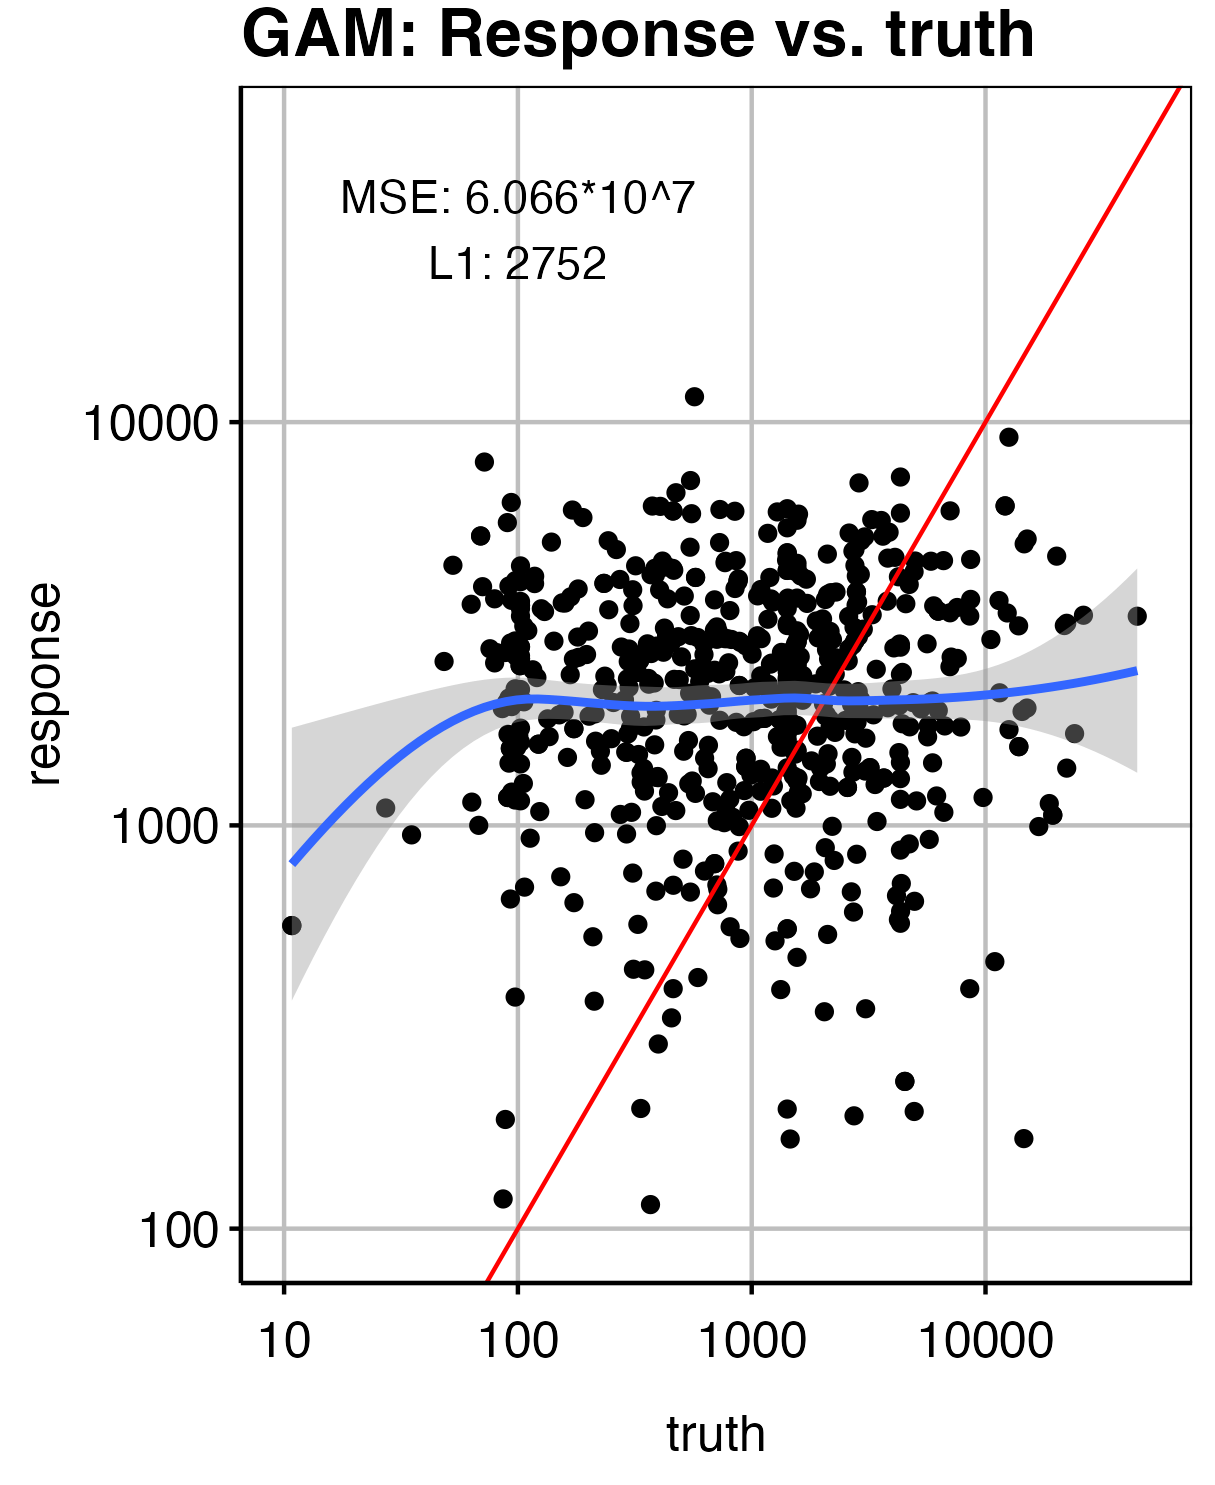
\includegraphics[width=0.3\textwidth]{figures/sev_p_gam.png} }}
    \subfloat[\centering]{{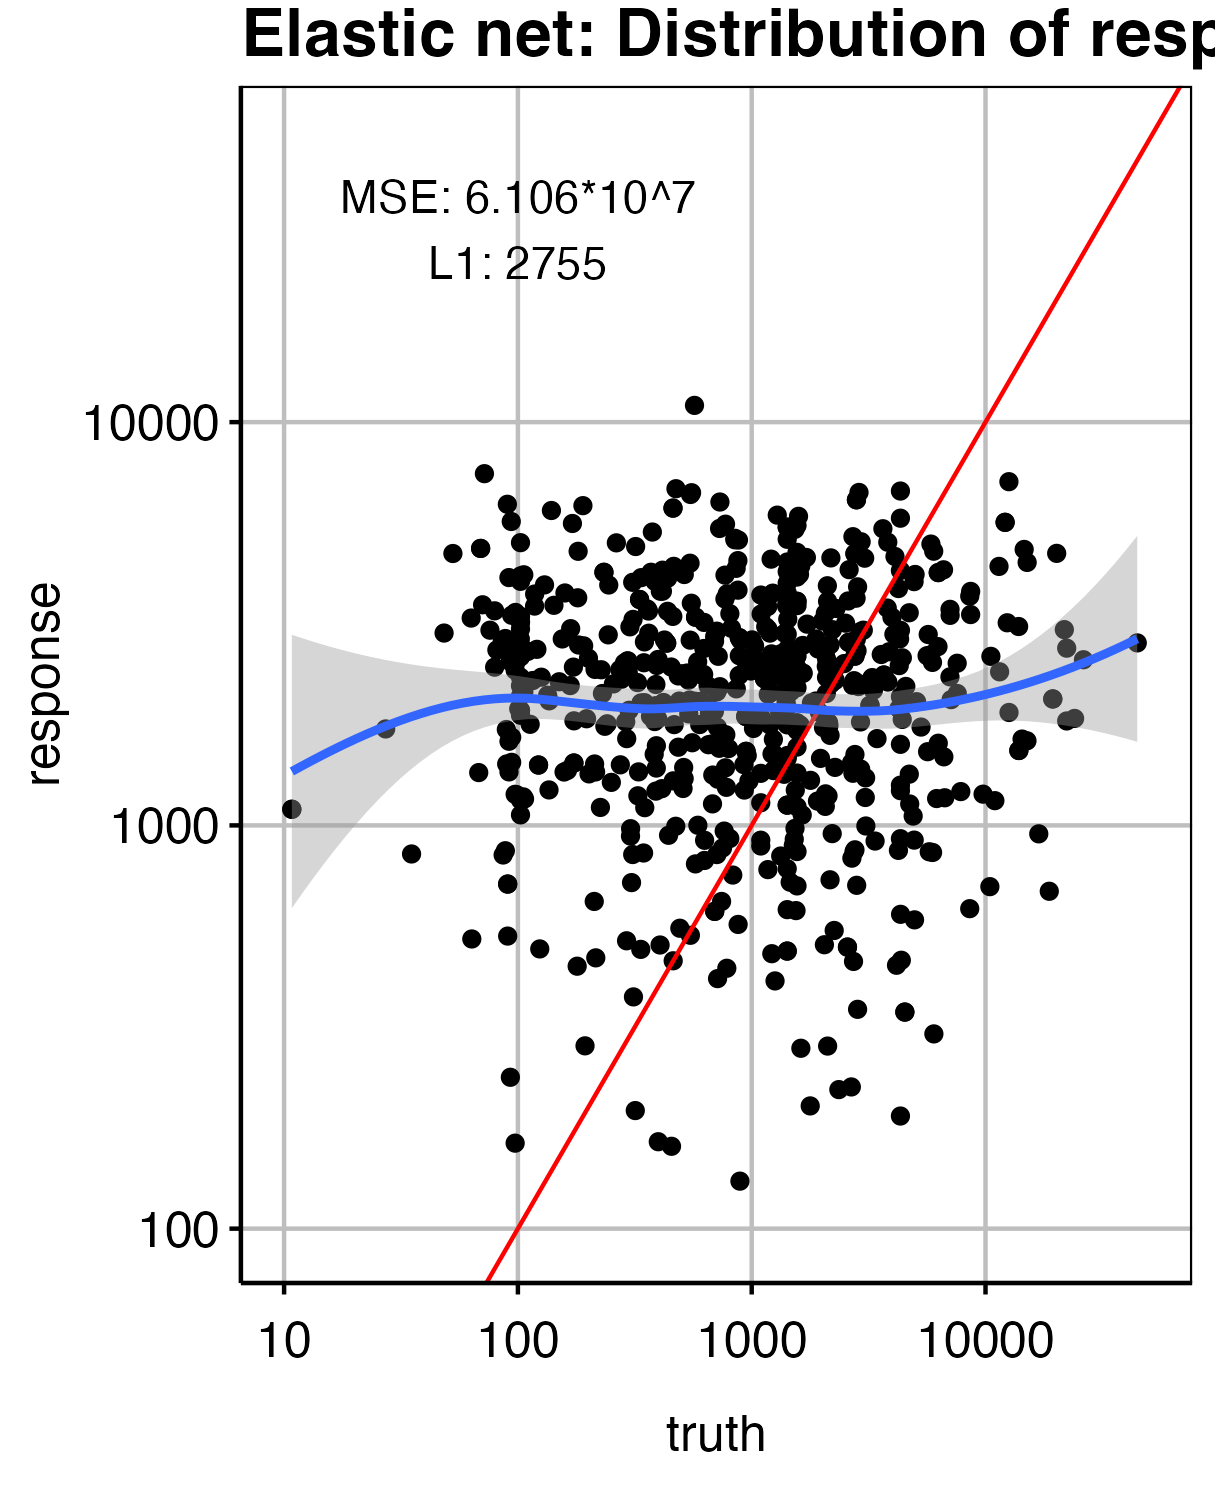
\includegraphics[width=0.3\textwidth]{figures/sev_p_glmnet.png} }}
    \subfloat[\centering]{{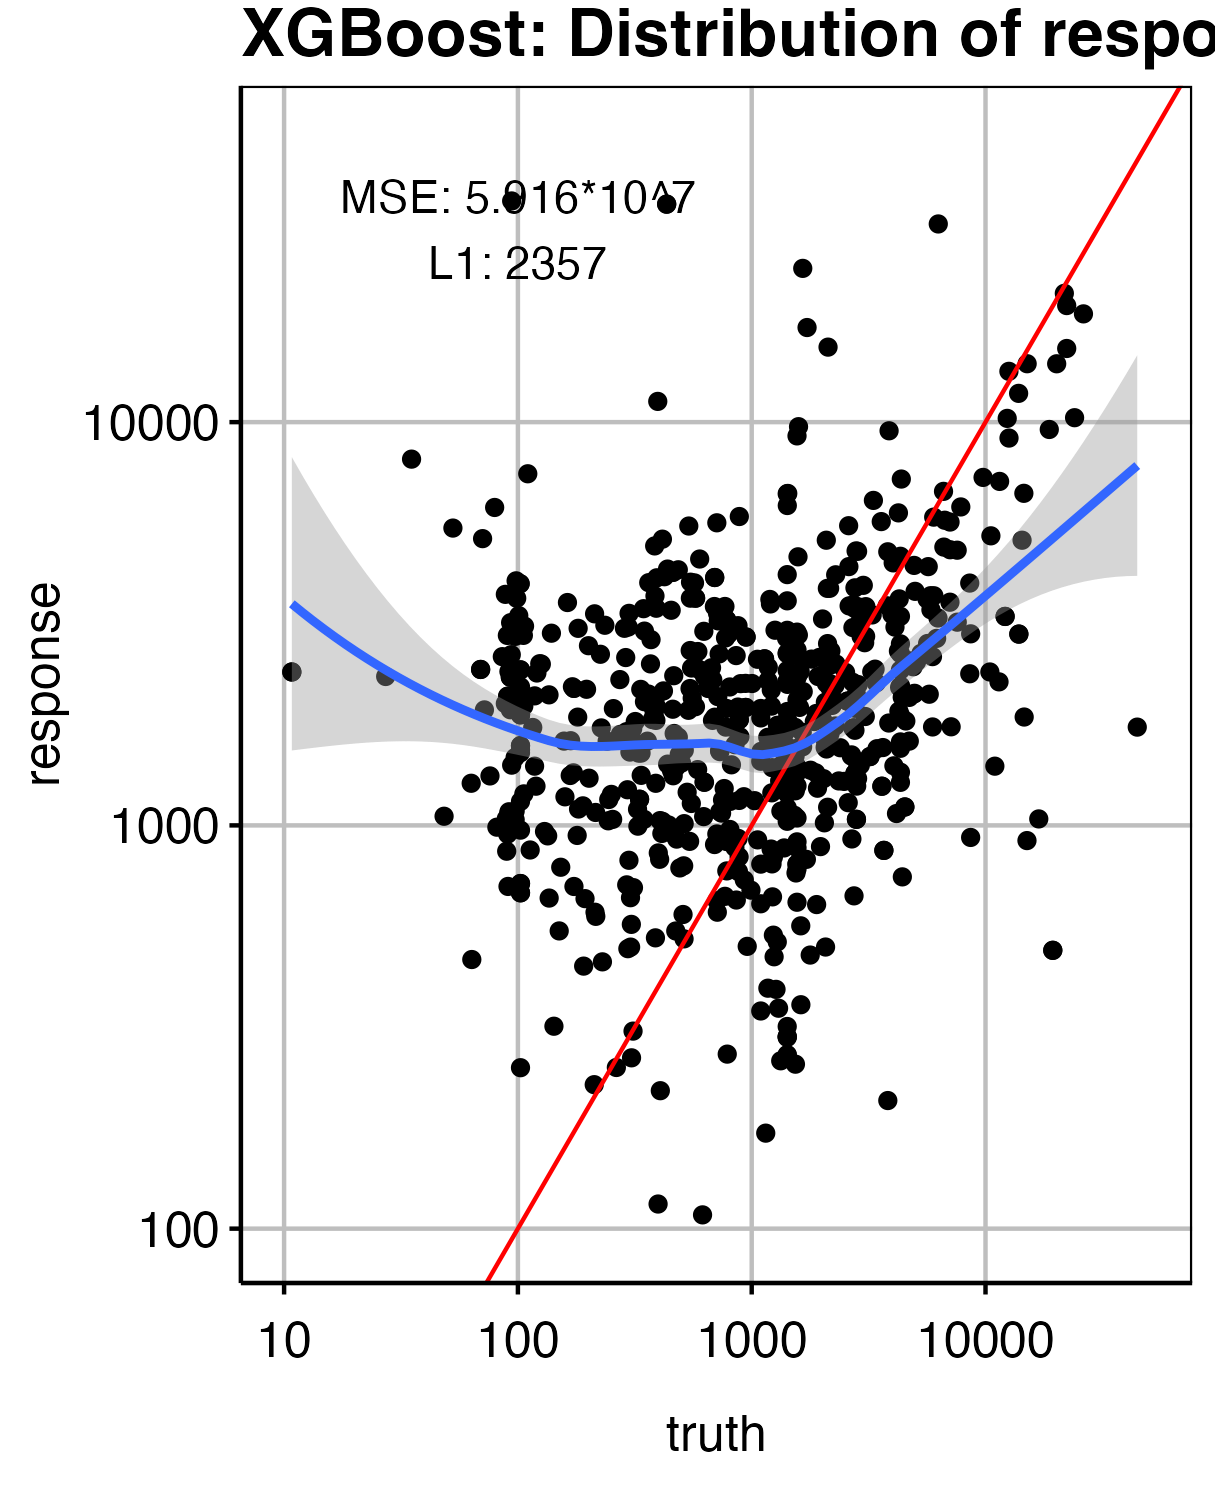
\includegraphics[width=0.3\textwidth]{figures/sev_p_xgboost.png} }}
    \qquad
    \subfloat[\centering]{{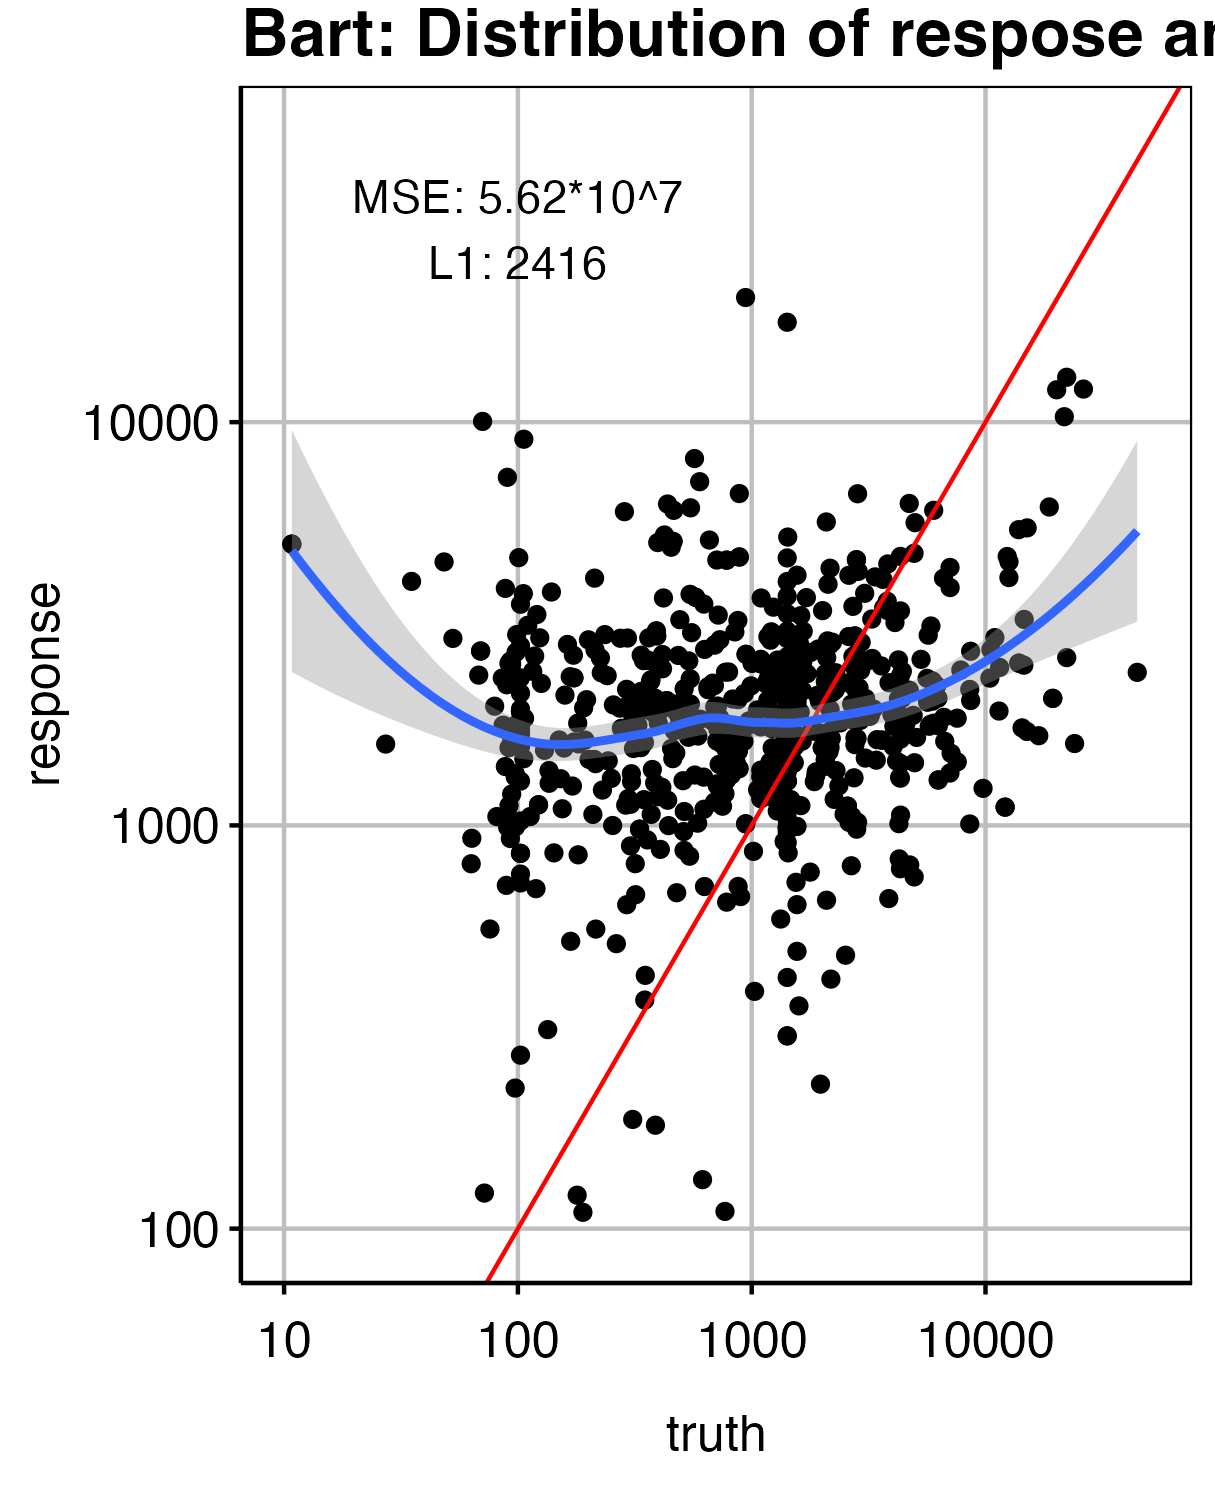
\includegraphics[width=0.3\textwidth]{figures/sev_p_bart.png} }}
    \subfloat[\centering]{{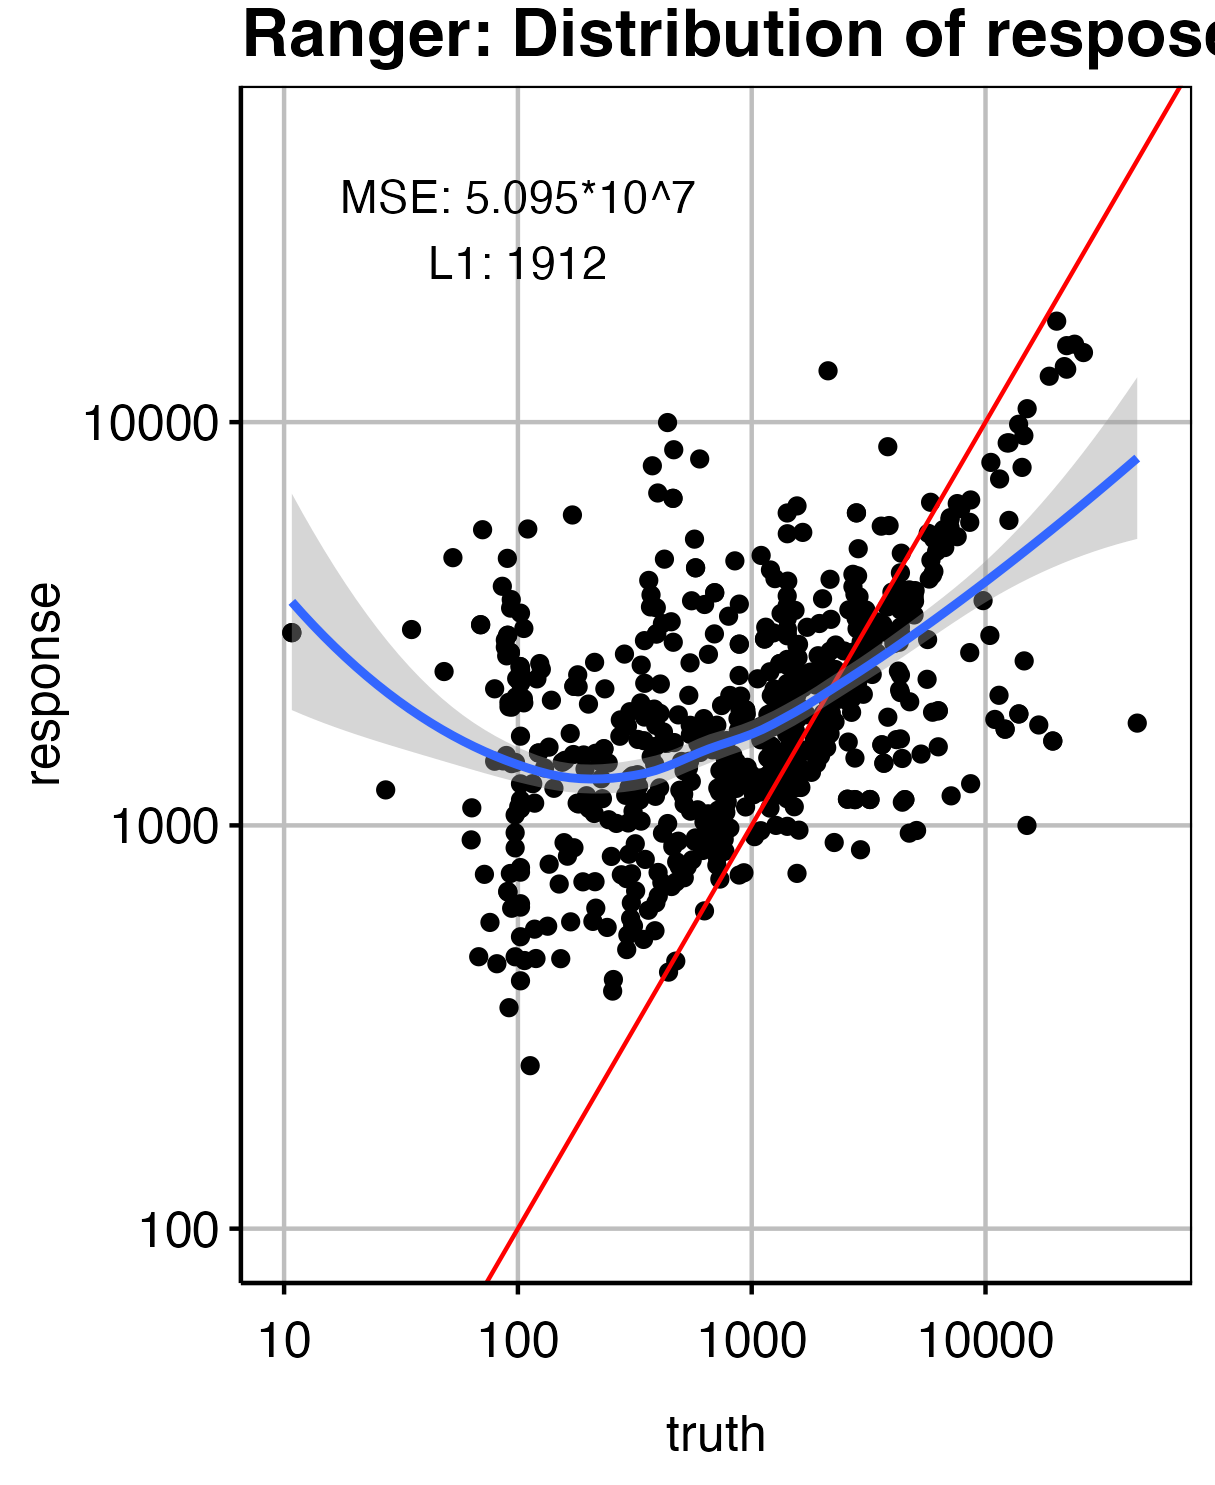
\includegraphics[width=0.3\textwidth]{figures/sev_p_ranger.png} }}
    \caption{Predictions for the five algorithms with x being the actual value and y being the estimate. The red line represent the mapping $y=x$.}
\end{figure}

\newpage

\hypertarget{comparing-the-frequency-models}{%
\subsection{Comparing the frequency
models}\label{comparing-the-frequency-models}}

\begin{figure}[h]
    \centering
    \subfloat[\centering]{{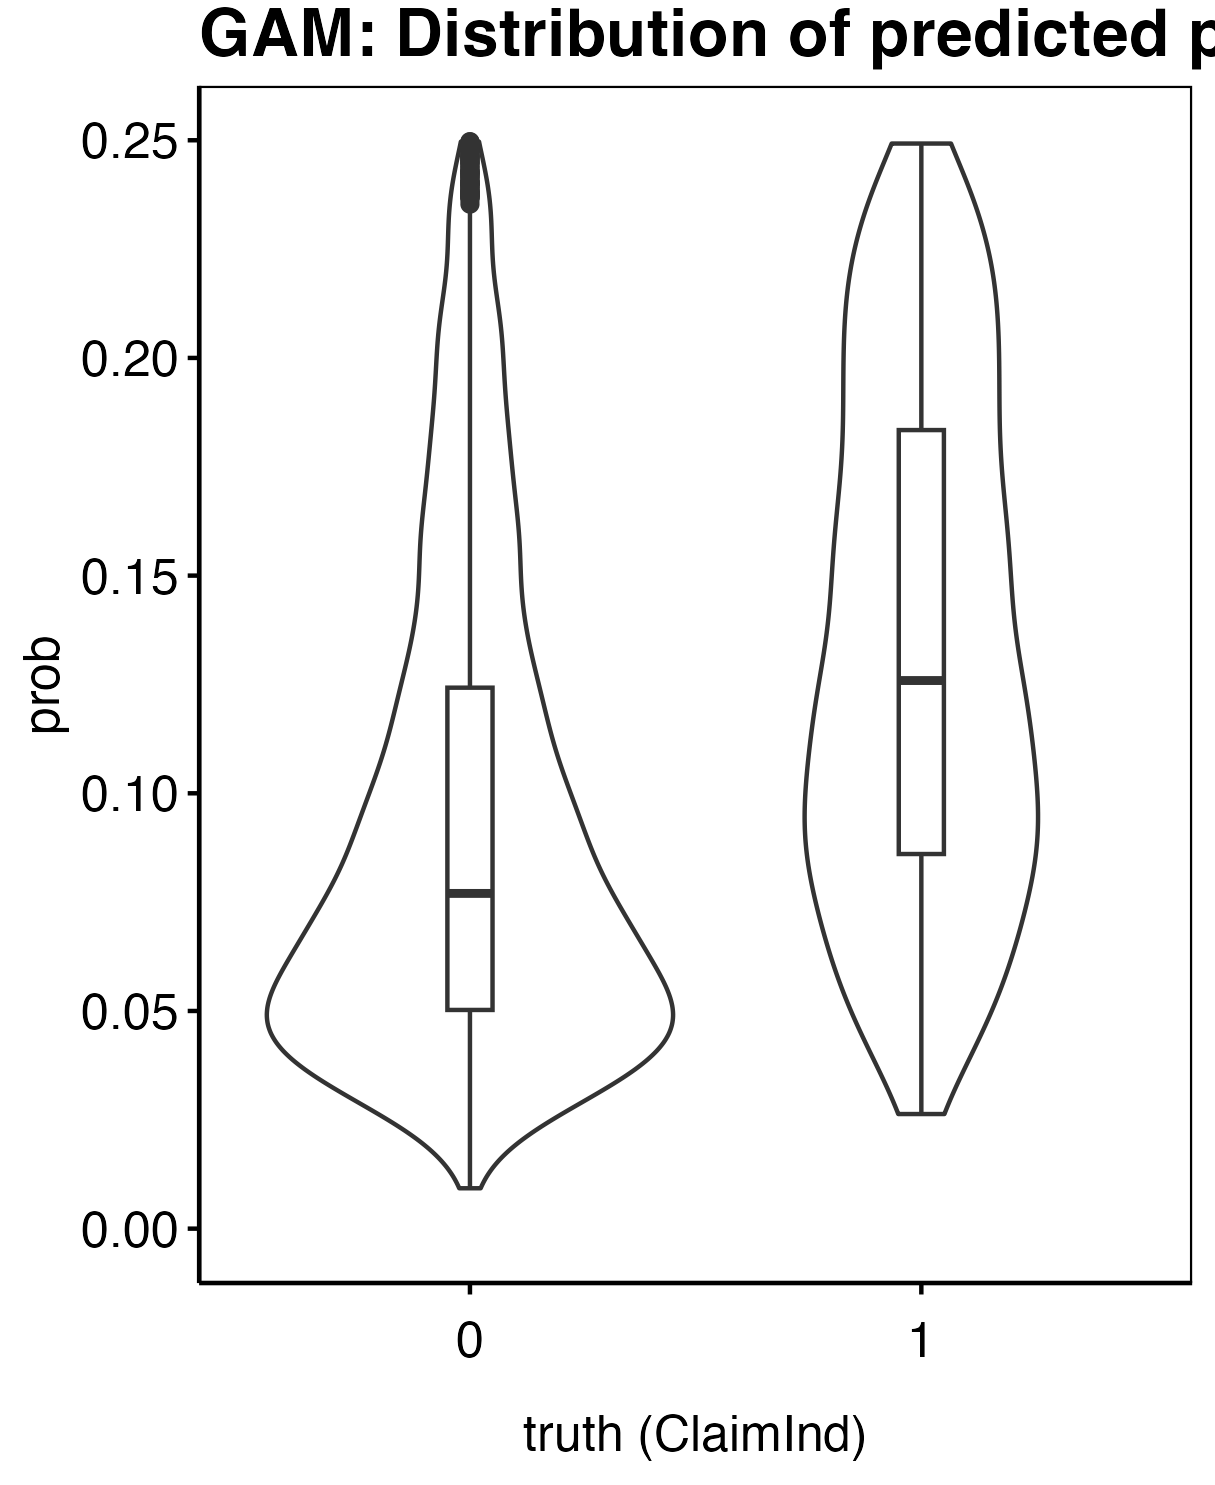
\includegraphics[width=0.3\textwidth]{figures/freq_p_gam.png} }}
    \subfloat[\centering]{{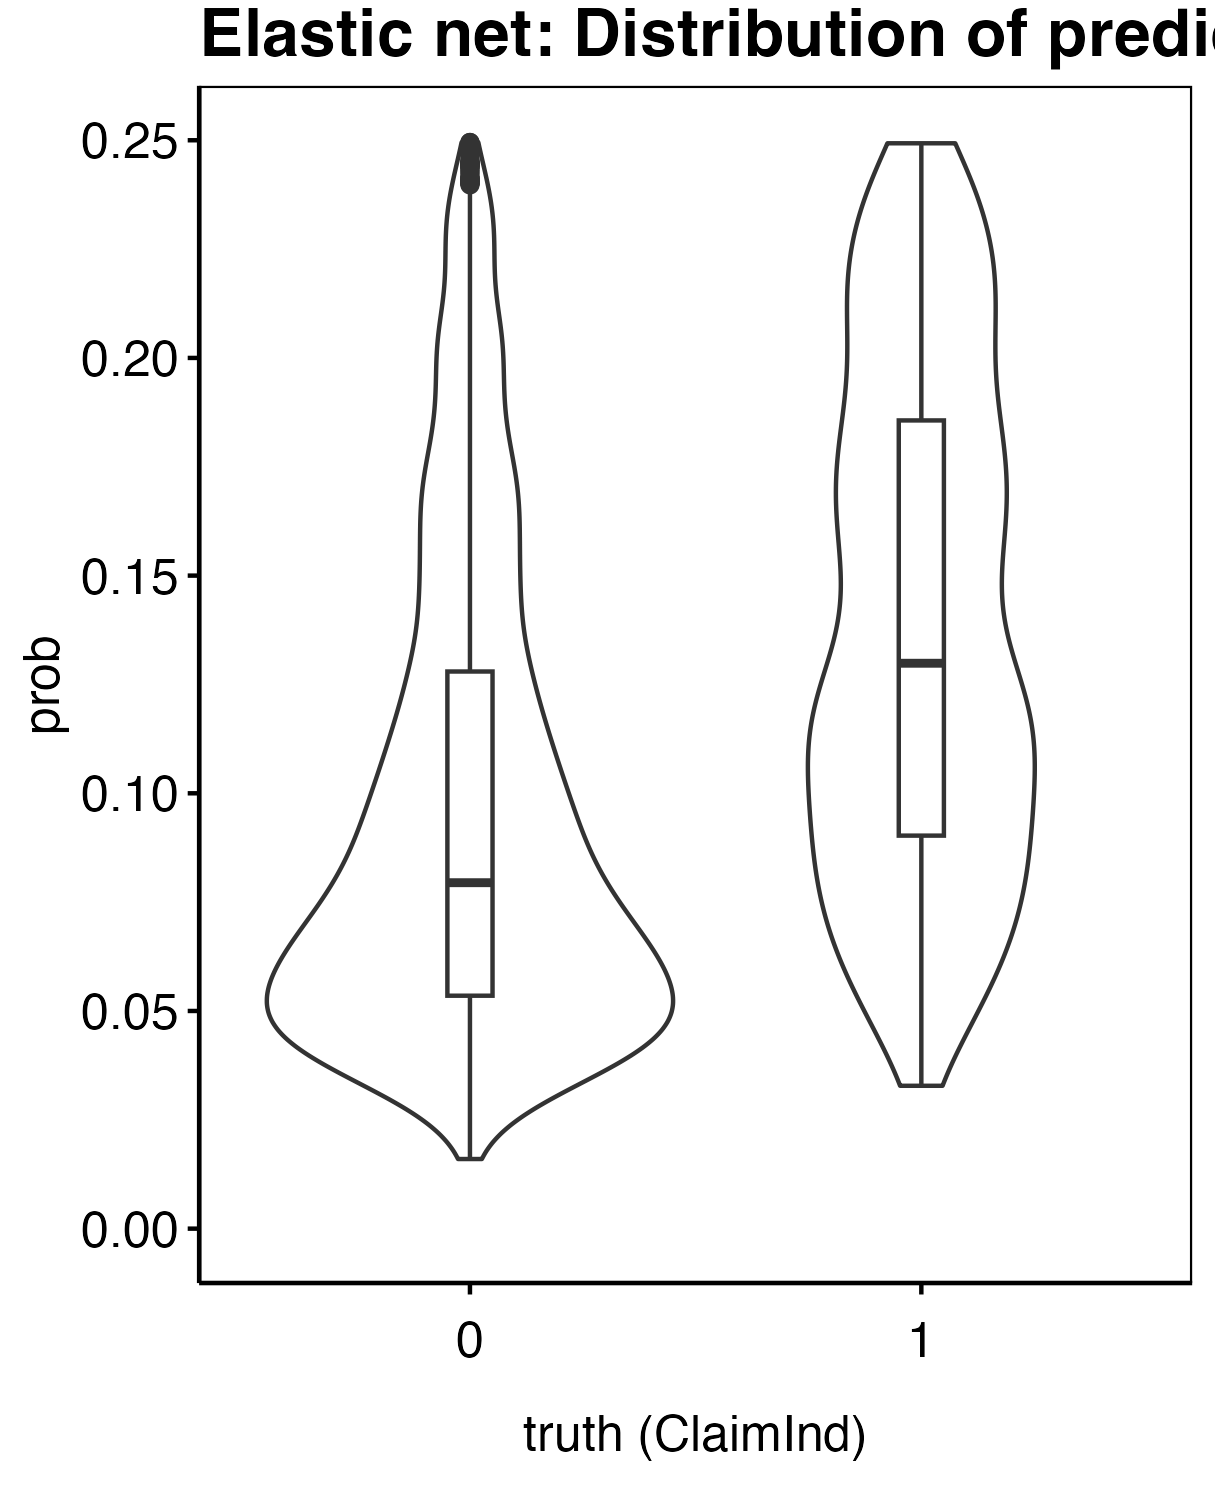
\includegraphics[width=0.3\textwidth]{figures/freq_p_glmnet.png} }}
    \subfloat[\centering]{{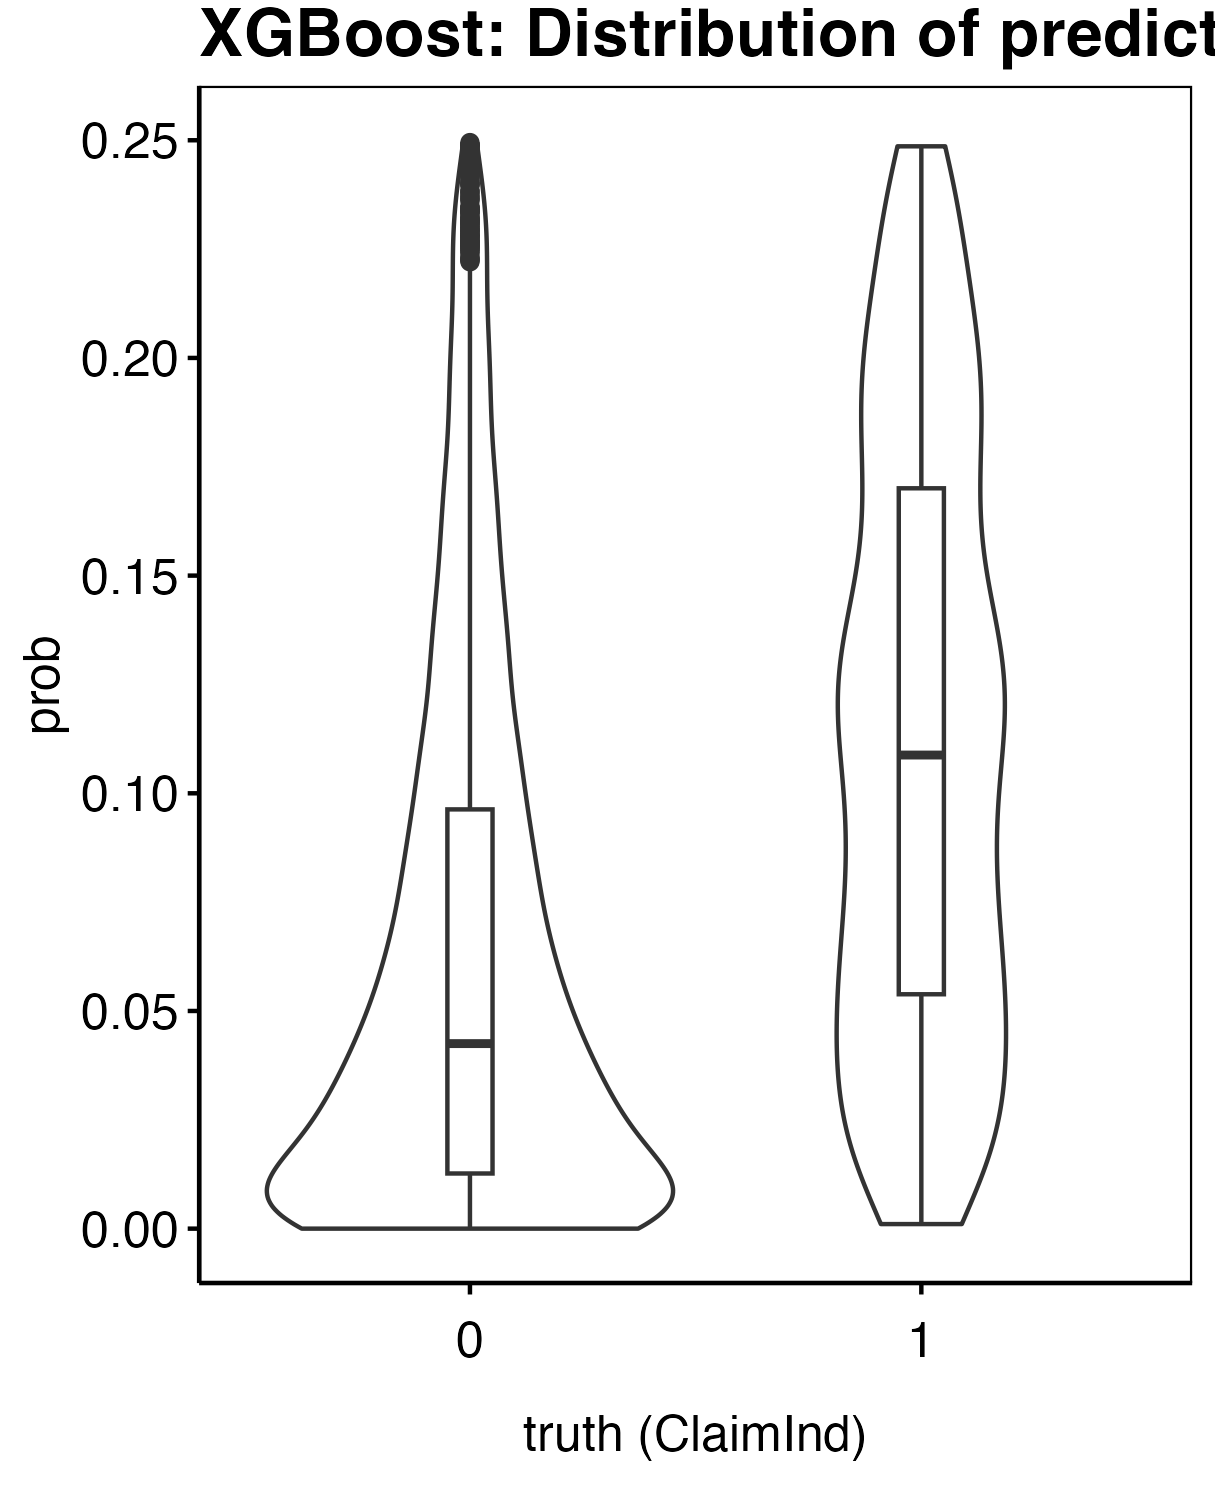
\includegraphics[width=0.3\textwidth]{figures/freq_p_xgb.png} }}
    \qquad
    \subfloat[\centering]{{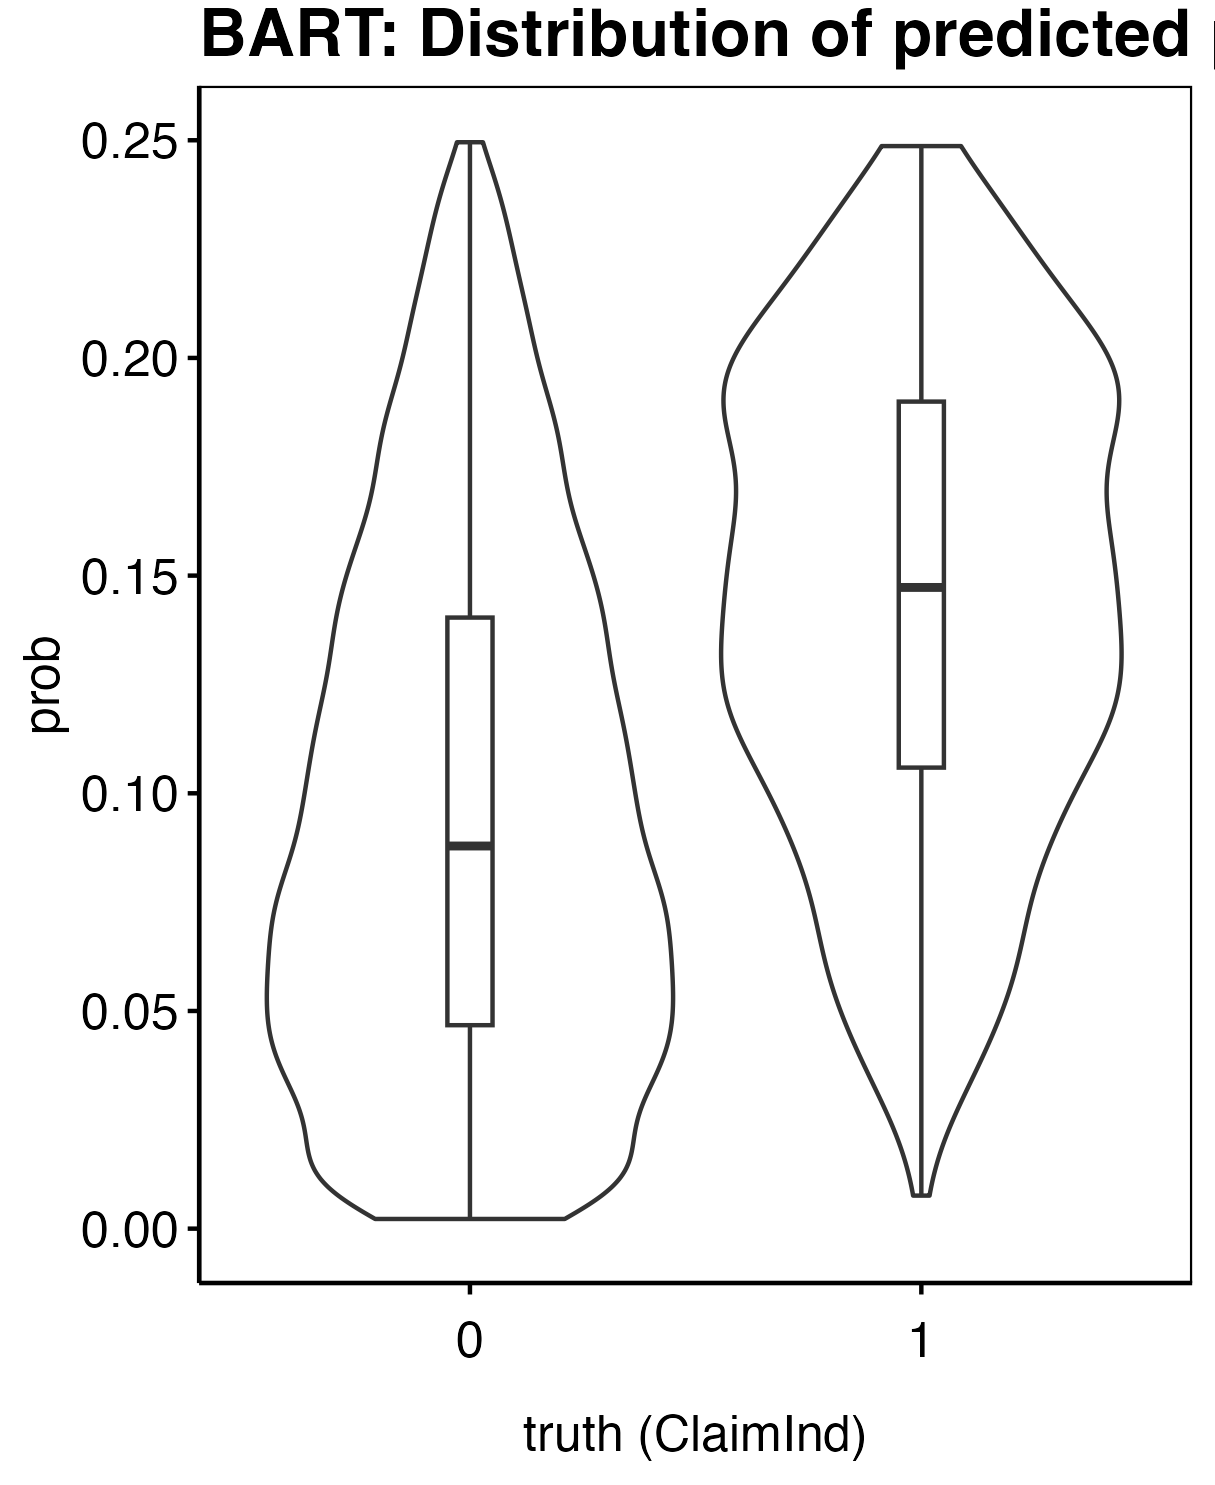
\includegraphics[width=0.3\textwidth]{figures/freq_p_bart.png} }}
    \subfloat[\centering]{{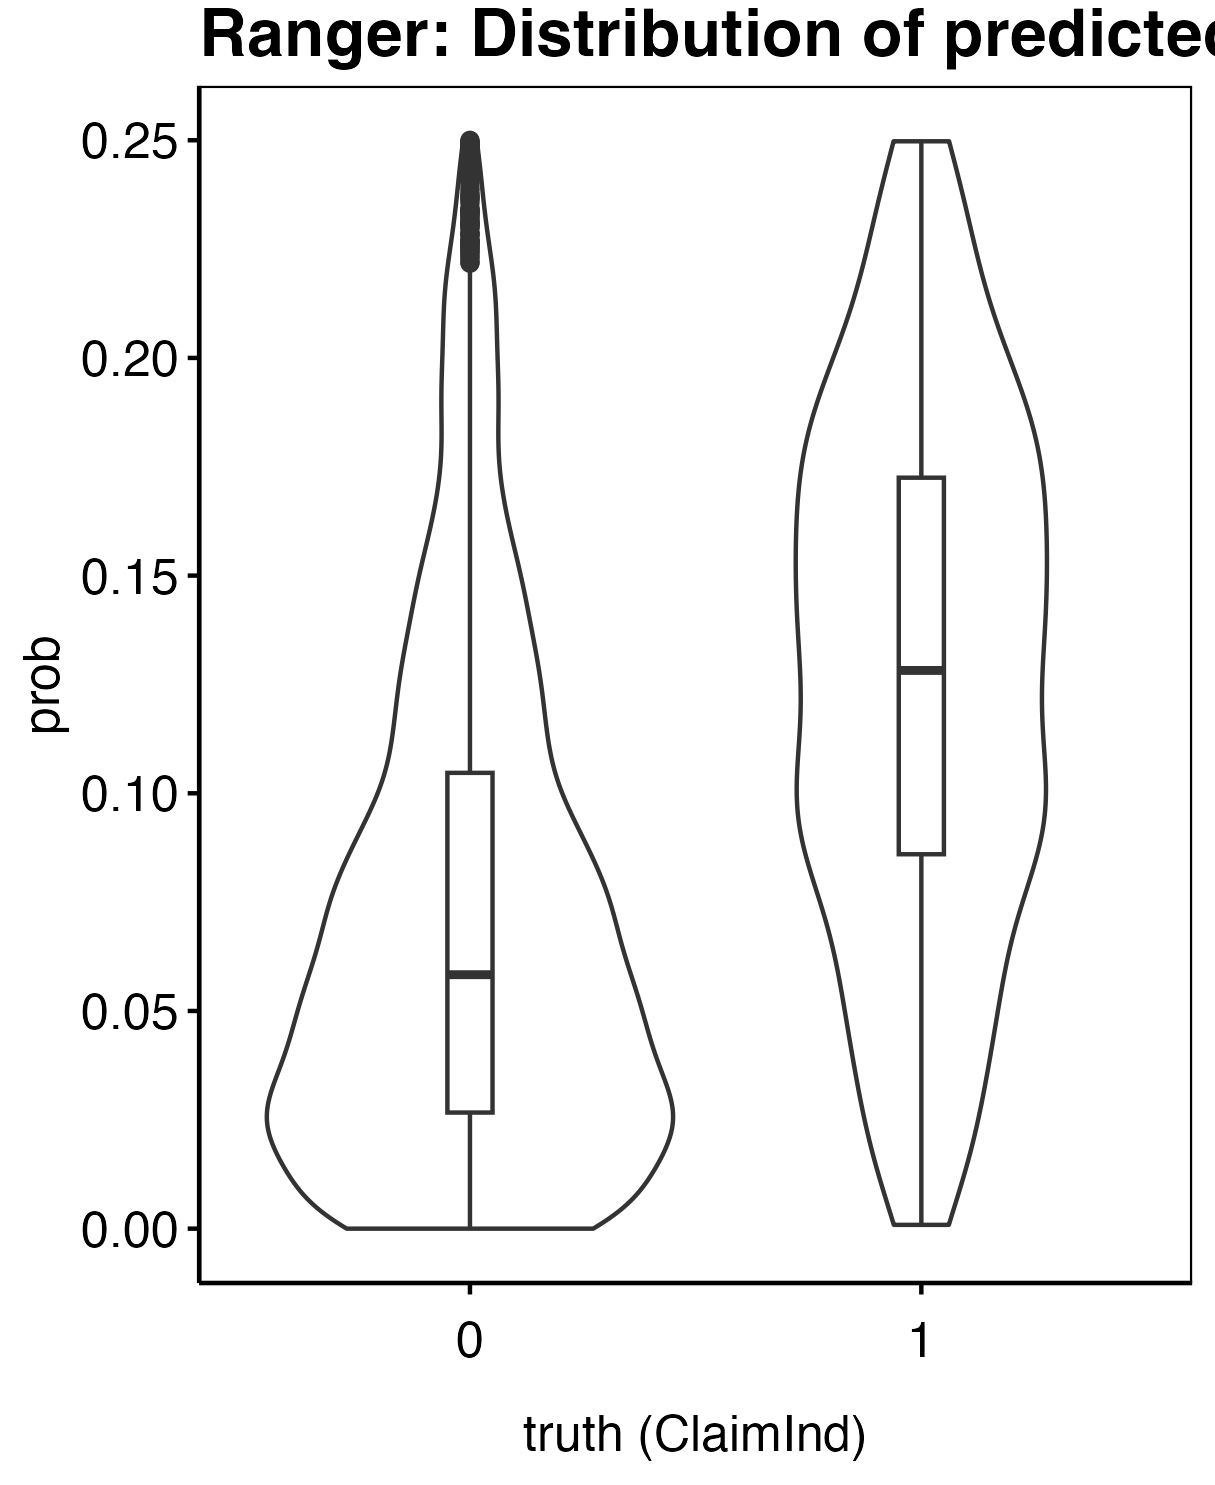
\includegraphics[width=0.3\textwidth]{figures/freq_p_ranger.png} }}
    \caption{Combined violin and boxplot of the predicted probabilities for non-claim and claim policies.}
\end{figure}

\end{document}